\documentclass[%
  a4paper,oneside,%
  %arial,
  11pt,% <10pt, 9pt>
  smallchapters,
  style=printdev,
  extramargin,
  %sender=bottom,
  green,% <orange, green, violet>
  rgb, <cmyk>
  %mono
  ]{tubsbook}

\usepackage[backend=biber,style=ieee,backref=true]{biblatex}

\addbibresource{Library.bib}

\usepackage{siunitx}
\sisetup{load-configurations = abbreviations,output-exponent-marker=\ensuremath{\mathrm{e}}}  
  
\usepackage{listings}  % for code stuff
\usepackage{minted}

\usepackage{booktabs}
\usepackage{multirow}

\usepackage{physics}

\usepackage{bbm} %for probability notation
\usepackage{subcaption}

\usepackage{tikz}
\usepackage{tikzit}
\input{MA.tikzstyles}
\newcommand{\rn}[2]{%% "rn": "remember node"
	\tikz[remember picture,baseline=(#1.base)]\node [inner sep=0] (#1)  {$#2$};%
}

%\usepackage{hyperref}

\usepackage{xcolor}

\definecolor{codegreen}{rgb}{0,0.6,0}
\definecolor{codegray}{rgb}{0.5,0.5,0.5}
\definecolor{codepurple}{rgb}{0.58,0,0.82}
\definecolor{backcolour}{rgb}{0.95,0.95,0.92}

\lstdefinestyle{mystyle}{
	language=Python,
    backgroundcolor=\color{backcolour},   
    commentstyle=\color{codegreen},
    morekeywords={self},
    keywordstyle=\color{magenta},
    numberstyle=\tiny\color{codegray},
    stringstyle=\color{codepurple},
    basicstyle=\ttfamily\footnotesize,
    breakatwhitespace=false,         
    breaklines=true,                 
    captionpos=b,                    
    keepspaces=true,                 
    numbers=left,                    
    numbersep=5pt,                  
    showspaces=false,                
    showstringspaces=false,
    showtabs=false,                  
    tabsize=2
}


\newcommand\pythonstyle{\lstset{
	language=Python,
    backgroundcolor=\color{backcolour},   
    commentstyle=\color{codegreen},
    morekeywords={self},
    keywordstyle=\color{magenta},
    numberstyle=\tiny\color{codegray},
    stringstyle=\color{codepurple},
    basicstyle=\ttfamily\footnotesize,
    breakatwhitespace=false,         
    breaklines=true,                 
    captionpos=b,                    
    keepspaces=true,                 
    numbers=left,                    
    numbersep=5pt,                  
    showspaces=false,                
    showstringspaces=false,
    showtabs=false,                  
    tabsize=2
}}


% Python environment
\lstnewenvironment{python}[1][]
{
\pythonstyle
\lstset{#1}
}
{}




%lstset{style=mystyle}

\usepackage{bm} 
\usepackage{amsmath}
 
\renewcommand{\familydefault}{\sfdefault}
\usepackage[utf8]{inputenc}
\RequirePackage{scrlfile}
\ReplacePackage{scrpage2}{scrlayer-scrpage}

\usepackage[ngerman,english]{babel}

\usepackage{lipsum} % Blindtext-Paket
\definecolor{InAGreen}{RGB}{172,193,58}

% Titelseiten-Elemente
\title{A Statistical Approach for the Fusion of Data and
Finite Element Analysis in Vibroacoustics}
\subtitle{Untertitel}
\author{Lucas Hermann}
%\logo{Institut fuer Lorem Ipsum}
\logo{
\includegraphics{InA-Logo-rgb.pdf}}
\titleabstract{\lipsum[2]}
\titlepicture{infozentrum.jpg}
% Rückseiten-Elemente
\address{%
  Herr Mustermann\\
  Schlossallee 1\\
  33333 Darmstadt}
\backpageinfo{%
  \lipsum[5]
}
\usepackage{pdfpages}								% Einbinden von PDF-Pages
\usepackage[colorlinks,pdfpagelabels,pdfstartview = FitH,bookmarksopen = true,bookmarksnumbered = true,linkcolor = black,plainpages = false,hypertexnames = false,citecolor = black] {hyperref}
\usepackage[figure]{hypcap} 

\begin{document}

%\maketitle[image,logo=left]%[<plain/image/imagetext>,<logo=left/right>]
%\makebackpage[trisec]%[<plain/info/addressinfo>]
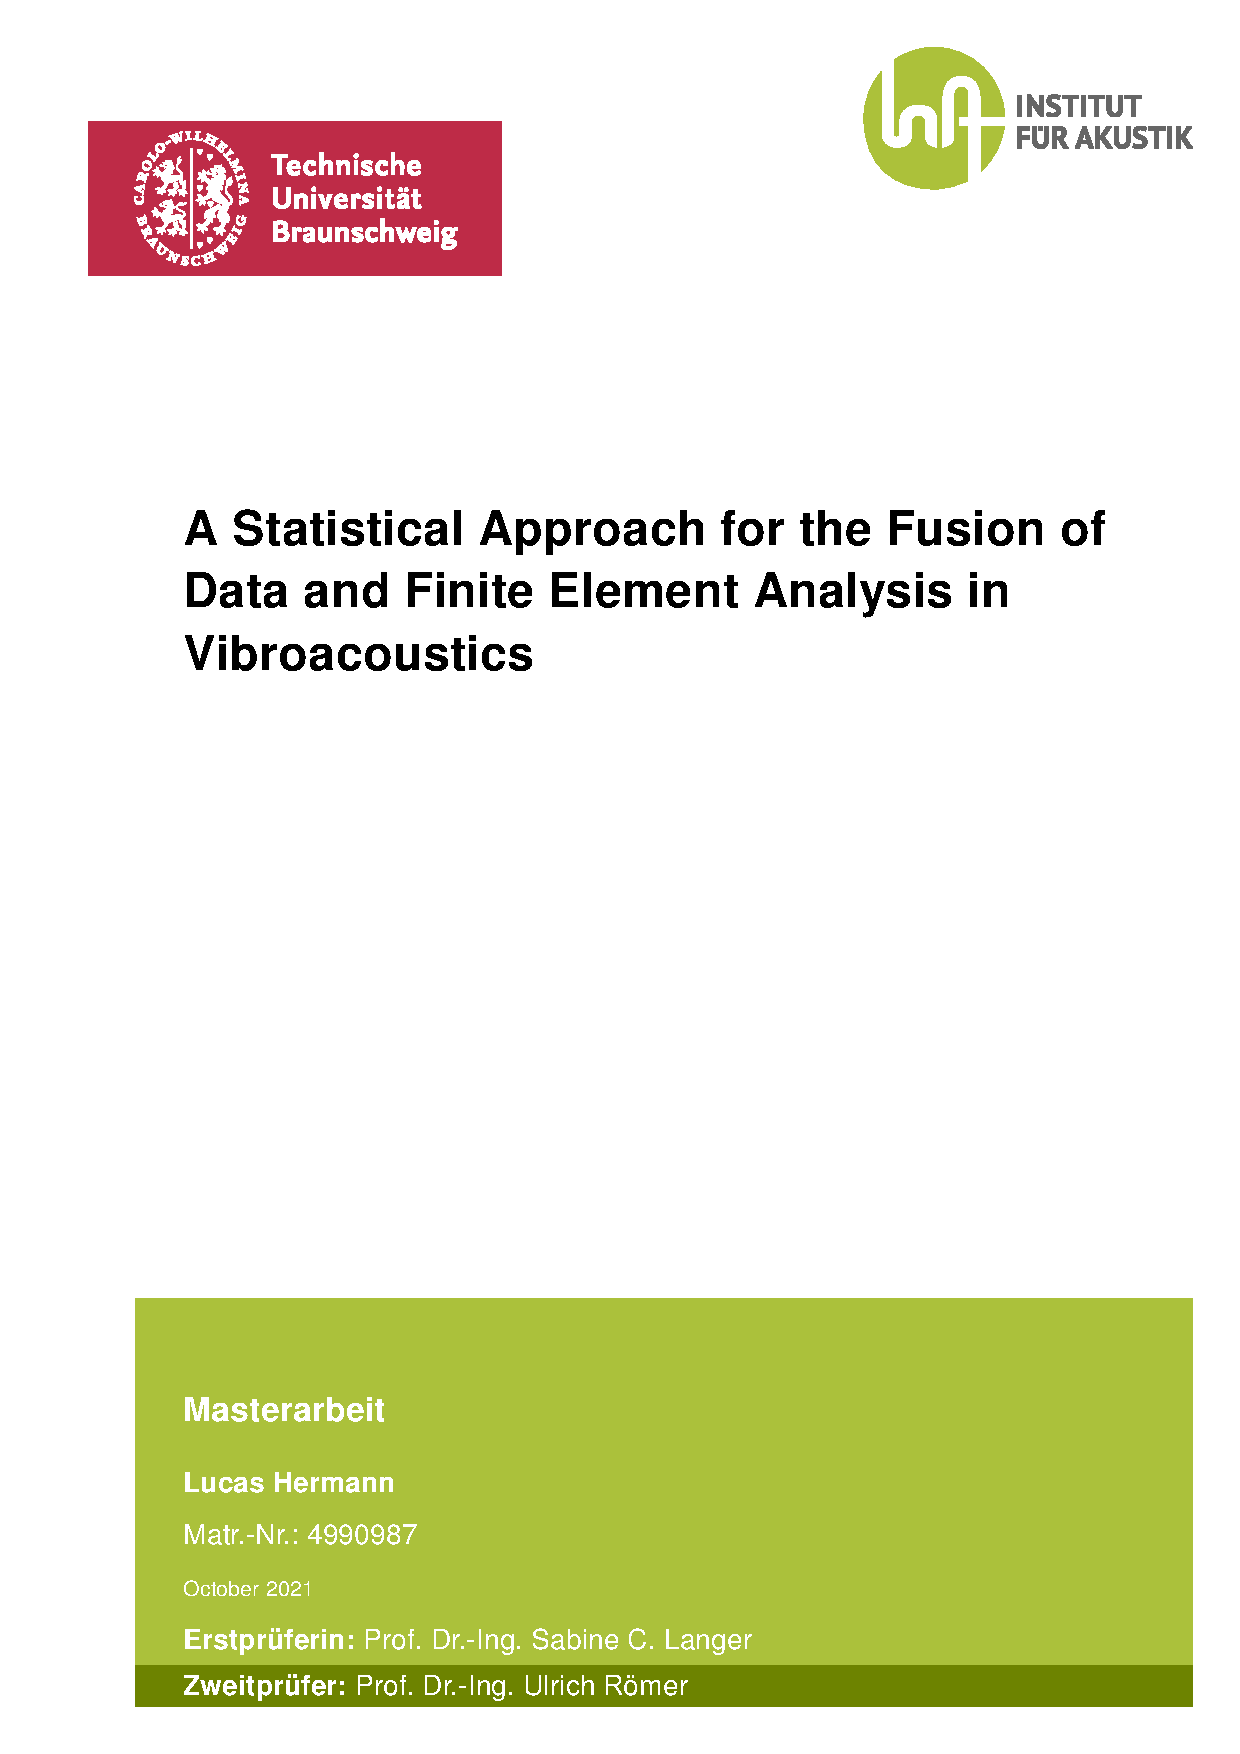
\includepdf[pages=-]{./Deckblatt/2099_StA_Name_Deckblatt.pdf}

\chapter*{Declaration}
Hiermit versichere ich, Lucas Hermann, durch meine Unterschrift, dass ich die
vorliegende Masterarbeit mit dem Titel ``<<Titel>>'' selbständig und ohne Benutzung
anderer als der angegebenen Hilfsmittel angefertigt habe. Alle Stellen, die wörtlich oder sinn-
gemäß aus veröffentlichten oder unveröffentlichten Schriften entnommen sind, habe ich als
solche kenntlich gemacht. Insbesondere sind auch solche Inhalte gekennzeichnet, die von
betreuenden wissenschaftlichen Mitarbeiterinnen und Mitarbeitern des Instituts für Akustik eingebracht wurden.

Die Arbeit oder Auszüge daraus haben noch nicht in gleicher oder ähnlicher Form dieser
oder einer anderen Prüfungsbehörde vorgelegen.

Mir ist bewusst, dass Verstöße gegen die Grundsätze der Selbstständigkeit als Täuschung
betrachtet und entsprechend der Prüfungsordnung geahndet werden.

\begin{flushright}
Braunschweig, \today
\end{flushright}

\vspace{2cm}
\hspace{2cm}\rule{5cm}{1pt}

\hspace{2cm}\small{Lucas Hermann} 

\chapter*{Abstract}
To increase the accuracy of an FEM model, statFEM is is used in a vibroacoustics scenario. An introduction to vibroacoustics, FEM, Gaussian Processes and statFEM is given before the methods are applied. A 2D vibroacoustics problem is solved via FEM and synthetic measurements are used to condition the FEM solution, which serves as a Bayesian prior, on. It is shown that already comparatively few sensor locations and observations per sensor lead to a much more accurate posterior model. 

\tableofcontents


\chapter{Introduction}

%\textcolor{tubsSecondary}{Dies ist ein Text in \texttt{tubsSecondary}.}
%\textcolor{tubsViolet}{Dies ist ein Text in \texttt{tubsViolet}.}
%\textcolor{tubsGreenDark}{Dies ist ein Text in \texttt{tubsGreenDark}.}\bigskip
A core discipline in engineering is numerical simulation. It is needed in basic research and in the design process of any product to reduce the amount of practical experiments which are costly and time-consuming. In a numerical simulation, the relevant processes of reality are abstracted by a mathematical model, which a computer is able to solve. \cite{Weisberg2015} However, a model is only able to describe reality up to a certain degree. It usually consists of a set of equations and corresponding parameters which can be tweaked in order to make it behave as closely to the desired functionality as possible or to match data from measurements. Uncertainty in the parameters can be propagated to the solution, leading to a probability density for the solution which assigns probabilities to different possible outcomes. However, as this is a valid approach, as soon as the real problem behaves in a more complex manner than the model is able to describe, the procedure is reaching its limits. The real behavior of the problem is not considered in the solution space of the model anymore.%The headroom given by the probability densities in the parameters just isn't enough to tweak them in a way that makes the model describe reality accurately. 
There is now a gap between model and reality which has to be filled.

A common approach to form a model in engineering is the Finite Element Method (FEM). At the base of it stands a partial differential equation (PDE), which is a model of reality itself. The PDE is simplified using so-called ansatz functions which have weights that are tweaked in order to get the most accurate picture of reality. Traditionally, the FEM is purely deterministic but, nevertheless, it is rather simple to form a Bayesian approach to FEM, in which the parameters and the solution are not scalars but random variables which have an underlying probability distribution. 
Recently, a method, called statFEM, was developed \cite{girolami2021}, which also allows for bridging the gap between a Bayesian FEM model and reality. This is in principle done by assuming the discrepancy between model and reality to behave in terms of a Gaussian Process (GP). A GP can be, unlike a probability distribution over a parameter, considered as a probability distribution over a whole function. Since there are no parameters left in the FEM model to tweak, this is the only way to go: The most suitable function to fill the model discrepancy gap has to be found without building another parameterized model. The GP is based on measurement data: By comparing the FEM model with observed data and then updating it in a Bayesian manner, a distribution over functions can be found, which makes the now updated FEM model behave more closely to reality.

In this thesis, a statFEM approach for the field of vibroacoustics is formulated. The physical problem under consideration is an acoustical cavity which is excited by a plate at its boundary. The behavior of the fluid inside the cavity is described by the Helmholtz equation and depends strongly on the chosen boundary conditions. Obviously, there is a lot of uncertainty involved in the modeling of the boundary conditions: It is not possible to completely describe the behavior of the vibrating plate or the partially absorbing walls of the cavity. Nevertheless, it is possible to measure the sound pressure inside the cavity: Assuming the sound field to behave in terms of a GP makes it possible to form a posterior solution with reduced model error and uncertainty using the measured data and the prior in form of the FEM solution. The statFEM approach is therefore, in order to reduce uncertainty, able to fuse an FEM simulation with measured data and also to give an approximation of the mentioned gap between model and reality.

In the first chapters, the theory behind GPs, the FEM and statFEM is explained thoroughly. Then, the methods are explained and validated using the textbook-example of the Poisson equation before they are applied to the more complex vibroacoustics problem. The behavior of the new model is explained and discussed in detail and information on possible use cases and limitations are given.


\chapter{FEM Solution of the Helmholtz Equation}
This thesis is based on two pillars: Solving the governing equation for acoustics using the Finite Element Method (FEM) and implementing a probabilistic approach using GPs and statFEM. For the first one, the equations for the Helmholtz equation and the FEM are going to be derived in this chapter.

An acoustic field is represented in time domain by the wave equation. It returns the acoustical pressure at a point in space $x$ for a time variable $t$.
The Helmholtz equation describes the wave equation in a time-independent manner, i.e. in frequency domain. It has a dependency on the frequency, so the goal is to solve the Helmholtz equation for a range of frequencies in order to obtain a frequency response plot which gives insight on the modal behavior of the system.

\paragraph{Literature Review}
\cite{langtangen2019} and \cite{larson2013} give a thorough explanation about the theoretical basis of the Finite Element Method. \cite{langtangen2016} gives details about the implementation of the FEM in Python using FEniCS. On a more abstract level, \cite{Lanczos1986} gives insight on variational formulations of PDEs which are essential for the FEM. For an explanation of FEM with a focus on acoustics, \cite{atalla2015} provides information and examples tailored to acoustics. \cite{moser2005} is a comprehensive standard reference for acoustics. 

\section{Wave Equation and Helmholtz Equation}
In a typical vibroacoustic problem, for example an interior structural acoustic coupling problem \cite{atalla2015}, there are usually two coupled domains: At first, there is some kind of solid medium which emits sound. The movement of that solid can be described within the field of elastodynamics using for instance (a) Bernoulli or Timoshenko beam theory for 1D beam-like structures, (b) Kirchhoff or Reissner-Mindlin plate theory for 2D plate-like structures. The focus of this thesis is another: As soon as the sound is emitted from the solid, the wave equation is used to describe the motions of sound waves through an acoustic medium such as air. 
The following closely follows \cite{larson2013} and \cite{moser2005}.
The behavior of a gas in a domain $\Omega$ can be described using the density $\rho$, the pressure $p$ and the velocity $v$. By changing the velocity or pressure locally by e.g. a speaker or a vibrating plate, this change is propagated through the medium. One can think of the gas as a system of infinitesimally small spring-mass systems. Deflecting one spring yields a deflection of the adjacent spring, or gas volume, but time-delayed due to the gas's inertia. That leads to a wave propagating through the medium. 
Newton's second law states that mass times acceleration equals force. If a gas volume is accelerated in one direction, that leads to a force on the neighboring particle \cite{moser2005}.
%
\begin{equation}
m \dot{v} = S  \left[  p(x) -p(x + \Delta x)  \right] 
\end{equation}
with $m$ the mass of the gas volume, $S$ the surface of the contact area of the two volumes  and $\Delta x$ the length of a gas volume in the direction of motion. Considering $m = \Delta x S \rho$ there holds
\begin{equation}
\rho \dot{v} = - \frac{p(x) -p(x + \Delta x)}{\Delta x} \; .
\label{eqn:waveEqDeriv1}
\end{equation}
Assuming interaction between infinitessimaly small gas particles and therefore taking the limit of the difference quotient in (\ref{eqn:waveEqDeriv1}) yields the differential quotient and hence
\begin{equation}
\rho \dot{v} = - \nabla p \;.
\label{eqn:Tragheitsges}
\end{equation}
$\nabla$ is the nabla operator $\left( \pdv{}{x_1},\pdv{}{x_2},...,\pdv{}{x_n} \right)$ which consists of the partial derivatives of the used coordinates. For cartesian coordinates, applied as a product to a quantity, it describes the gradient of the quantity, i.e.
\begin{equation}
\nabla p = \mathrm{grad}p = \left( \pdv{p}{x},\pdv{p}{y},\pdv{p}{z} \right) \;.
\end{equation}


If a volume is expanded, the pressure of the contained gas drops and vice versa. Therefore a change of volume is proportional to a negative change of pressure. An expanding volume is also represented by the divergence of the velocity \cite{larson2013}. Imagine quickly pulling a piston out of an airtight cylinder: The air particles will move in the direction of the piston movement while the volume expands and the pressure drops. Hence, there holds
\begin{equation}
\dot{p} = -k \nabla u
\label{eqn:Constit}
\end{equation}
with $k$ a proportionality constant dependent on the medium.
Differentiating (\ref{eqn:Constit}) with respect to $t$ yields 
\begin{equation}
\ddot{p} = -k \nabla \dot{u} \;.
\end{equation}
Inserting \ref{eqn:Tragheitsges} and considering $c^2 = k/\rho$ there holds for the acoustic wave equation
\begin{equation}
\ddot{p} = c^2 \nabla^2 p 
\label{eqn:WaveEq}
\end{equation}
which involves derivatives in both time and space. To obtain a general representation of the behaviour of a pressure field independent of time, the Helmholtz equation can be derived as follows.
Considering a separation ansatz \cite{westermann2015}
\begin{equation}
p(x,t) = X(x) \cdot T(t) \; ,
\end{equation}
there holds for \ref{eqn:WaveEq}

\begin{align}
X(x) \cdot \pdv[2]{T(t)}{t} &= c^2 \nabla^2 X(x) \cdot T(t)\\
\frac{1}{T(t)} \pdv[2]{T(t)}{t} &= c^2 \frac{1}{X(x)} \nabla^2 X(x) = const. = - \omega^2 \; .
\end{align}
With the wave number $k = \omega / c$ 
\begin{equation}
\nabla^2 X(x) + k^2 X(x) = 0
\end{equation}
is the Helmholtz equation which is a representation of the wave equation independent of time \cite[p. 1083 ff.]{arens2015}.
%
With $p [\SI{}{\pascal}]$ the pressure field and $k$ the wave number it is in the following going to be referred to by
\begin{equation}
\nabla^2 p + k^2 p = 0 \;.
\label{eqn:Helmholtz}
\end{equation}
With $\omega$[\SI{}{\radian}] the angular frequency, $f$[\SI{}{\per\s}] the frequency and $c_0[\SI{}{\metre\per\s}]$ the speed of sound in the considered medium $k$ is defined as
\begin{equation}
k = \frac{\omega}{c_0} = \frac{2 \pi f}{c_0} \;.
\end{equation}
(\ref{eqn:Helmholtz}) is solved as a boundary value problem which means that the behavior of the system has to be described beforehand for the boundaries of the calculation domain. That is done using boundary conditions.



\paragraph{Boundary Conditions}
The following closely follows \cite{atalla2015}. There are three different types of boundary conditions: Dirichlet, Neumann and Robin type. Neumann boundary conditions are also called natural boundary conditions because these automatically arise in the equation while deriving the weak form of the problem. Dirichlet boundary conditions, on the other hand, don't. They are called essential boundary conditions and have to be applied by hand after deriving the weak form and building the linear system of equations.
%\paragraph{Dirichlet}

The Dirichlet boundary condition for the Helmholtz equation is simply a prescribed pressure $\bar{p}(x)$ at the $\Gamma_D$ part of the boundary:
\begin{equation}
p(x) = \bar{p}(x) \quad \forall x \in \Gamma_D \;.
\end{equation}



	
%\paragraph{Neumann}
The Neumann boundary condition at $\Gamma_N$ reads
\begin{equation}
\dv{p(x)}{n} = \rho \omega^2 \vec{U(x)} \cdot \vec{n} \quad \forall x \in \Gamma_N
\end{equation}
with $\vec{U}$ the displacement and $\vec{n}$ the outer normal direction of the surface. It can be thought of as a piston moving with circular frequency $\omega$ at the boundary which creates a velocity and pressure change. Choosing a homogeneous Neumann BC $\dv{p(x)}{n} = 0$ resembles a reflecting boundary. The part of the boundary, where a homogeneouos Neumann BC is applied, is going to be called $\Gamma_{N0}$.

%\paragraph{Robin}
The Robin or impedance boundary condition at $\Gamma_R$ reads
\begin{equation}
\dv{p(x)}{n} + ik \beta p(x) = 0 \quad \forall x \in \Gamma_R
\end{equation}
with $\beta$ the specific normalized acoustic admittance. The Robin boundary condition is also called impedance boundary conditions because an acoustic impedance can be simulated what leads to e.g. partially reflecting walls.

Figure \ref{fig:BCEx} shows an example on how boundary conditions could be applied on a 2D domain. $\Gamma_{N0}$ boundary conditions are the mentioned natural boundary conditions which don't have to be applied explicitly. Still, a Neummann boundary condition $\Gamma_{N}$ can be imposed onto the system which behaves differently. 
Figure \ref{fig:BCTh} shows the setting chosen in this thesis: All walls are reflecting and on the left side of the domain a Neumann boundary conditon is imposed which is used to model the previously mentioned sound source. 


\begin{figure}[!ht]
\begin{center}
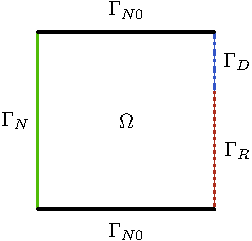
\includegraphics[width=0.4\textwidth]{pics/BCsExample}
\caption{Two dimensional representation of various boundary conditions. In this example, the left side is a Neumann boundary, the upper and lower boundaries are totally reflecting and the right side consists of an impedance BC and a Dirichlet BC.}
\label{fig:BCEx}
\end{center}
\end{figure}


\begin{figure}[!ht]
\begin{center}
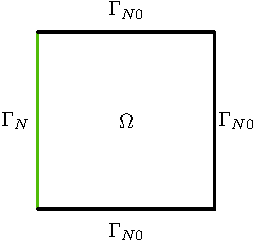
\includegraphics[width=0.4\textwidth]{pics/BCsThesis1}
\caption{Boundary Conditions of the problem for this thesis. A Neumann boundary is applied on the side of the domain. It is going to be modeled as a GP. The rest of the boundary is considered as reflecting, i.e. $\Gamma_N = 0$.}
\label{fig:BCTh}
\end{center}
\end{figure}

FEniCS \cite{langtangen2016} is a Python/C++ library for solving PDEs with the Finite Element Method. It makes it easy to go directly from the variational formulation of a problem to solving it.
Using FEniCS, the boundary conditions can be applied to the system of equations by 
%
\begin{minted}
[
frame=lines,
framesep=2mm,
baselinestretch=1.2,
bgcolor=backcolour,
fontsize=\footnotesize,
linenos
]
{python}
class BoundaryX_L(SubDomain):
	self.tol = 1E-14
	def inside(self, x, on_boundary):
		return on_boundary and near(x[0], 0, tol)# and (x[1] < 0.3)
boundary_markers.set_all(9999) # all markers default to zero.
bxL = BoundaryX_L()
bxL.mark(boundary_markers,0) # left side is marked as "0"
ds = Measure('ds', domain=self.mesh, subdomain_data=boundary_markers) #define a new operator for the boundary
\end{minted}
%
%
This construction can then be used when defining the variational problem:
%
\begin{minted}
[
frame=lines,
framesep=2mm,
baselinestretch=1.2,
bgcolor=backcolour,
fontsize=\footnotesize,
linenos
]
{python}
U = 0.0001 #Piston displacement
g = self.rho * self.omega**2 * U
a = inner(nabla_grad(self.u), nabla_grad(self.v))*dx - self.k**2 * inner(self.u,self.v)*dx #variational Problem
L = (self.v*g)*ds(0) # 0 is the chosen boundary marker
\end{minted}

Having the problem defined mathematically, the equations can now be prepared for being solved by FEM.




\section{The Classical Finite Element Method}


The Finite Element Method (FEM) is a procedure which makes it simple to approximately solve Partial Differential Equations (PDEs) which would be very hard or even impossible to solve analytically. As the name suggests, the calculation domain is split into $n_e$ individual elements on which the PDE is approximated using so-called ansatz functions. The process of dividing the domain in $n_e$ elements is called discretization. The polynomial degree of the ansatz functions and the number of elements determine the accuracy of the approximation. In order to set up the FEM, the PDE needs to be in the so-called variational, or "weak", formulation. 
After discretization of the domain and deriving the weak formulation, the PDE can be approximated on the individual elements. Assembling the element matrices yields a global system of equations which can, after boundary conditions are applied, be solved for the unknown vector.


\subsection{Integral and Weak Formulation}
- Explain Vector spaces
- Test function: needs to obey the dirichlet conditions
- explain what a bilinear and a linear form is!


The Helmholtz equation is the so-called governing equation for the problem considered in this thesis. The governing equation is given in the strong form and is usually of higher order. This property makes it hard to solve the equation, both analytically and numerically. For being able to apply the FEM, the order of the PDE has to be lowered. That is archieved by first bringing the equation in the weak, or also called variational, formulation.
One way to derive the weak formulation of the governing equation is the method of weighted residuals. 
\paragraph{The Weigthed Residuals Method}
The residual $R$ is the difference between approximation and exact solution. The exact solution is usually not known. Therefore the residual is formed by inserting the approximation of the solution into the PDE. The result is non-zero and a measure for the quality of the approximation \cite{langtangen2019}. To increase the quality, the residual has to be minimized. 
An FEM approximation, see \ref{chap:ApproxFem} for details, uses FEM basis functions which are weighted with some factors $c_j$. The goal is finding the factors which minimize $R$. The seeked approximated solution vector to the Helmholtz equation $\bm{p}$ is part of a space $V$ which is spanned by the FEM basis functions $\varphi_i$. Demanding the scalar product of the residual and a test function $v$ to be zero
\begin{equation}
(R,v) = 0, \quad \forall v \in V \;,
\end{equation}
i.e. demanding that they are orthogonal, can be used to minimize $R$. $V$ can be spanned by the FEM basis functions as well. Nevertheless, it doesn't necessarily need to be defined in the same space as $\bm{p}$. Using the same space would be called the Galerkin method. Applying the Weighted Residuals Method to the Helmholtz equation is executed as follows.
At first the strong formulation (PDE) is multiplied with the test function $v$ and integrated over the domain $\Omega$ to get the so-called integral formulation:
\begin{equation}
\int_{\Omega} v \nabla^2 p \,\mathrm{d}\Omega + \int_{\Omega} k^2 pv \,\mathrm{d}\Omega = 0
\label{eqn:IntForm}
\end{equation}
%

The approximated function within an element, here it is $p$, is called the trial function. It is part of a constrained space of trial functions or termed as the trial space. The test function $v$ is also part of a test space. Usually, trial and test spaces are chosen to be the same. Both trial and test spaces have to fulfill the Dirichlet boundary conditions imposed on the PDE.
The Helmholtz equation and therefore also the now formed integral formulation contain derivatives of second order. However, the FEM works by adjoining individual element functions to a global function. Therefore, the global solution is a piecewise polynomial \cite{langtangen2019} what causes problems when calculating higher-order derivatives because those become discontinuous. In consequence, integration by parts is performed using Green's first identity \cite[pp. 53,54]{atalla2015} on the higher-order terms to get lower order derivatives. It makes use of the divergence theorem, also called Gauss's theorem:

\begin{equation}
\int_{\Omega}  \nabla \cdot \vec{F} \,\mathrm{d}\Omega = \oint_{\Gamma} \vec{F} \cdot \vec{n} \,\mathrm{d}\Gamma \; .
\label{eqn:DivTheo}
\end{equation}
It states that all of the sources and sinks inside a domain (which generate divergence) must be equal to the amount of flux over the boundary of that domain. 
By defining  $F = vu$ with $u = \nabla p$ and making use of the product rule of vector calculus $\nabla \cdot (v u) = v \nabla \cdot u + u \cdot \nabla v$ there holds for Green's first identity
\begin{equation}
\oint_{\Gamma} v \nabla p \,\mathrm{d}\Gamma = \int_{\Omega} \nabla p \cdot \nabla v \,\mathrm{d}\Omega + \int_{\Omega}  v\nabla^2 p \,\mathrm{d}\Omega \; .
\end{equation}
%
Applying it to (\ref{eqn:IntForm}) yields
\begin{equation}
-\int_{\Omega} \nabla p \cdot \nabla v \,\mathrm{d}\Omega + \oint_{\Gamma} v \nabla p  \,\mathrm{d}\Gamma+ \int_{\Omega} k^2 pv \,\mathrm{d}\Omega = 0
\label{eqn:WeakHelmholtz}
\end{equation}
with the boundary of the domain $\Gamma$.
The resulting equation is now called the weak formulation as opposed to the strong formulation since the trial function now only needs to be differentiable once less often.
The boundary term can be decomposed into three parts
\begin{equation}
\oint_{\Gamma} v \nabla p  \,\mathrm{d}\Gamma = \oint_{\Gamma_D} v \nabla \bar{p}  \,\mathrm{d}\Gamma + \oint_{\Gamma_N} v (\rho \omega^2 \vec{U}\vec{n})  \,\mathrm{d}\Gamma + \oint_{\Gamma_R} v(-ik\beta p)  \,\mathrm{d}\Gamma
\end{equation}
with $\oint_{\Gamma_D} v \nabla \bar{p}  \,\mathrm{d}\Gamma = 0$ for the Dirichlet part because if the value at the boundary is known, then $\bar{f}$ is a scalar quantitity of which the derivative in outward normal direction of the boundary is zero.

\subsection{Discretization}
In this thesis, two different orders of domains are used: In a simple example, a 1D domain is going to serve as an illustration. For the actual vibroacoustics problem, a 2D domain will be examined. In this chapter, the FEM discretization for both orders is discussed.
%
Discretization means that the domain $\Omega$ is split into $n_e$ individual elements $\Omega^{(e)}$
\begin{equation}
\Omega = \bigcup_{e=1}^{n_e} \Omega^{(e)} \quad e = 1,...,n_e \;.
\end{equation}
This holds not only for 1D meshes but for 2D and 3D meshes as well.
For 1D meshes, such as in Figure \ref{fig:1DDom}, each element has two so-called nodes. This is because between the element boundaries a linear function is spanned which needs two support points to be defined.  In a 2D domain, an element would have 3 nodes, see Figure \ref{fig:2DDom}. Also different shapes of elements, e.g. quaratic elements with 4 nodes, are possible. The collection of nodes is called a mesh. The total number of nodes in a 1D mesh is $n = n_e + 1$, in a 2D mesh it is $n = n_x \times n_y$ with $n_x$ and $n_y$ the number of nodes in each coordinate. The minimum degree of the used function is determined by the weak form: It always needs to be differentiable, therefore a constant approximation function would not work \cite{atalla2015}. 

Figures \ref{fig:1DDom} and \ref{fig:2DDom} illustrate the discretization of a 1D and 2D domain, respectively.  For the 1D domain, the first ansatz functions are sketched: It is visible that for each node there is an ansatz function that yields the value $1$ only at that node and $0$ at all other nodes in the domain.
%
\begin{figure}[!ht]
\begin{center}

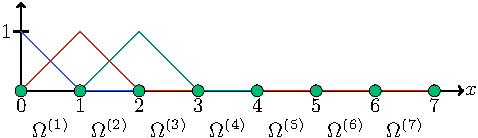
\includegraphics[width=0.6\textwidth]{pics/1dDomain}
\caption{A discretized 1D domain with nodes in green and linear ansatz functions shown for the first four nodes. The ansatz functions are 1 on their respective nodes and are 0 on all other nodes.}
\label{fig:1DDom}

\end{center}
\end{figure}
%
\begin{figure}[!ht]
\begin{center}

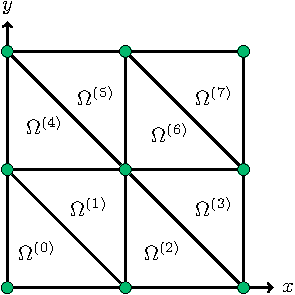
\includegraphics[width=0.4\textwidth]{pics/2dDomain}
\caption{A discretized 2D domain with nodes in green. Also here, the ansatz functions are defined so that they are 1 at their respective nodes and zero at all other nodes.}
\label{fig:2DDom}

\end{center}
\end{figure}
%
The finer the mesh, i.e. the more elements are used in a domain, the closer the FEM approximation comes to the exact solution. Since computing very fine meshes is computationally expensive, a convergence study is conducted in order to find the element size from which on smaller element sizes don't result in more accurate results.

Using FEniCS, a 1D mesh can be created by calling
\begin{minted}
[
frame=lines,
framesep=2mm,
baselinestretch=1.2,
bgcolor=backcolour,
fontsize=\footnotesize,
linenos
]
{python}
self.dom_a = 0.0 #domain boundaries
self.dom_b = 1.0
self.ne	= 60 #number of elements
self.mesh = IntervalMesh(self.ne,self.dom_a,self.dom_b) #define mesh
\end{minted}
The interval of the mesh and the desired number of elements have to be provided.

A 2D mesh can, for example, be obtained by calling
\begin{minted}
[
frame=lines,
framesep=2mm,
baselinestretch=1.2,
bgcolor=backcolour,
fontsize=\footnotesize,
linenos
]
{python}
self.a,self.b = 2,2
self.mesh = UnitSquareMesh(self.a,self.b) #define mesh
\end{minted}
In this case a unit square is chosen what means that the domain size will be quadratic and of length $1.0$ in every direction. $2$ elements were chosen for every dimension what leads to a mesh looking like \ref{fig:2DDom}. Of course every desired 2D shape can be used as a mesh.

\subsection{Approximation and Building Element Matrices}
\label{chap:ApproxFem}
In FEM, the values between nodes within an element are interpolated with basis functions $\varphi_i$. 
For each degree of freedom in the domain an FEM basis function is defined. By weighing those basis functions, the solution can be approximated with 
\begin{equation}
p(x_i) = \sum_{j = 1}^n c_j  \varphi_j(x_i) = f(x_i) \; .
\label{eqn:WeighingFunction}
\end{equation}
(\ref{eqn:WeighingFunction}) means, that the value of one particular point $x_i$ is the sum of all products of all weight coefficients $c_j$ and test functions $\varphi_j$ evaluated at that point. If now orthogonal basis functions are used, as it is commonly the case in FEM, (\ref{eqn:WeighingFunction}) simplifies as described below. One popular choice of FEM basis functions is the Lagrange family of polynomials. The right hand side $f(x_i)$ does, in practice, describe the source term of the PDE which does not depend on $p(x)$.

\paragraph{Lagrange Polynomials}
Following \cite{langtangen2019}.
Lagrange polynomials are one possible choice for FEM basis functions and are used in this thesis. They can be calculated for any desired degree $N$ and their main property is that they are $1$ at only a single node on the domain, $0$ at all other nodes and that they are nonzero on only a very limited fraction of the domain, as opposed to e.g. basis functions constructed from $\sin$ and $\cos$ terms. They are used as an interpolation between given points which means that the polynomial always exactly goes through the given points. The behaviour at all other points is determined by the definition of the Lagrange polynomial
\begin{equation}
\varphi_i(x) = \prod_{j=0,j\neq i}^N \frac{x-x_j}{x_i-x_j} \;.
\end{equation}
They are frequently used in FEM because there holds, if at $x_s$ there is a node of the mesh 
\begin{equation}
\varphi_i(x_s) = \delta_{is}, \quad \delta_{is}  =     \left\{ \begin{array}{rcl} 1 & \mbox{for}& i = s  \\ 0 & \mbox{for} & i \neq s\end{array}\right .
\end{equation}
which means that the polynomial is only $1$ at one node in the domain. At all other nodes it is $0$. Between nodes the Lagrange polynomial is spanned. This behavior simplifies (\ref{eqn:WeighingFunction}), if $x_i$ is the location of a node of the mesh:
\begin{equation}
p(x_i) = \hat{p}_i \varphi_i(x_i) = \hat{p}_i \;.
\end{equation}
The weight factor is therefore the approximated value at the node.
Another asset of using polynomials with $\varphi_i(x) = 0$ in most parts of the domain is that they lead to sparse matrices which can be solved much quicker than densely packed ones.
%
Now, to apply it to the weak form of the Helmholtz equation (\ref{eqn:WeakHelmholtz}), an approximation ansatz has to be made for both the trial and the test function. There holds for each element, if the same basis functions are used for both trial and test spaces,
\begin{align}
\begin{split}
\tilde{p} &= \bm{\varphi^T} \hat{\bm{p}} \\
\tilde{v} &= (\bm{\varphi^T} \delta\hat{\bm{p}})^T
\end{split}
\label{eqn:FEMAnsatz}
\end{align}
with $\delta\hat{\bm{p}}$ an arbitrary variation [Langer CompAc] of the pressure $\hat{\bm{p}}$, which gets cancelled out later on because the test function is present in every term.
Inserting (\ref{eqn:FEMAnsatz}) in the weak form, considering no Robin boundary conditions, results in
\begin{equation}
\sum_e \int_{\Omega_e} (\nabla \bm{\varphi} \nabla \bm{\varphi}^T)\,\mathrm{d}\Omega_e \hat{\bm{p}} -k^2 \sum_e \int_{\Omega_e} (\bm{\varphi} \bm{\varphi}^T)\,\mathrm{d}\Omega_e \hat{\bm{p}} = \rho \omega^2 \sum_e \int_{\Gamma_{e,N}} \bm{\varphi} U_n \,\mathrm{d}\Gamma_{e,N} \;.
\label{eqn:DiscretizedFEM}
\end{equation}
The sum $\sum_e$ means assembling the global system of matrices out of individual element matrices. In short, (\ref{eqn:DiscretizedFEM}) can be written as
\begin{equation}
\left( \sum_e \bm{K}_1^e - k^2 \sum_e \bm{K}_2^e \right)\hat{\bm{p}} = \rho \omega^2 \sum_e \bm{f}^e
\end{equation}
With $\bm{K}_1^e$ and $\bm{K}_2^e$ the elemental system matrices and $\bm{f}^e$ the elemental source vector. After assembly there holds for the global linear system
\begin{equation}
(\bm{K}_1 - k^2 \bm{K}_2) \hat{\bm{p}} = \rho \omega^2 \bm{f}
\label{eqn:LinSys}
\end{equation}
which is now to be solved for $\hat{\bm{p}}$.
To illustrate the assembly process, the so-called dynamic stiffness matrix $\bm{A}$ is introduced as
\begin{equation}
\bm{A} = (\bm{K}_1 - k^2 \bm{K}_2) \;.
\end{equation}
It is assembled using the individual matrices $\bm{A}^e$ for each element as visible in (\ref{eqn:Assembly}).
The goal is to solve the linear system of equations for the weight factors of the basis functions $p$, also called the degrees of freedom.
% It can be notated as
%\begin{equation}
%\sum_j A_{i,j} c_j = b_i
%\end{equation}
%with
%\begin{align}
%A_{i,j} &= \varphi_j(x_i), \\
%b_i &= f(x_i) \;.
%\end{align}
The calculation is usually done for one element at a time. Thereby arises an element matrix $A^{(e)}$ whose individual entries can be computed as
\begin{equation}
A_{r,s}^{(e)} = \int_{\Omega^{(e)}} \nabla \varphi_r \nabla \varphi_s \, \mathrm{d}\Omega^{(e)} - k^2 \int_{\Omega^{(e)}} \varphi_r \varphi_s \, \mathrm{d}\Omega^{(e)}
\end{equation}
with $r,s$ the indices of the individual nodes in an element. For 1D linear Lagrange elements, i.e. elements with two nodes each having one degree of freedom per node, a $2\times 2$ matrix results and for 1D quadratic Lagrange elements with three nodes each a $3\times3$ matrix results.
%
Also the right hand side vector, now called $\bm{b}$, is computed element-wise using
\begin{equation}
b_r^{(e)} = \rho \omega^2 \int_{\Omega^{(e)}} \int_{\Gamma_{e,N}} \varphi_r U_n \,\mathrm{d}\Gamma_{e,N} \;.
\end{equation}


The element matrices are then assembled to a global system matrix. Within an element, the coordinates of the nodes are $[0,...,d]$ with $d$ the dimension of the element. For linear elements, the coordinates are $[0,1]$. For assembly they need to be mapped to the global coordinate system. This is accomplished by using a mapping function, noted as $q$ which maps $[r,s]$ of the elements to $[i,j]$ in the global system: $i=q(e,r)$ and $j = q(e,s)$ with $e$ the number of the element. For the global system matrix there now holds
\begin{equation}
A_{q(e,r), q(e,s)} =  A_{r,s}^{(e)}
\end{equation}
for adding the entries of an element matrix to to global matrix.
The resulting matrix after assembly is sparse, here for three elements with linear ansatz functions:
\begin{equation}
A_{q(e,r), q(e,s)}  =
\begin{bmatrix}
\textcolor[rgb]{0.49,0.83,0.13}{A_{0,0}^{( 0)}} & \textcolor[rgb]{0.49,0.83,0.13}{A}\textcolor[rgb]{0.49,0.83,0.13}{_{0,1}^{( 0)}} & 0 & 0\\
\textcolor[rgb]{0.49,0.83,0.13}{A}\textcolor[rgb]{0.49,0.83,0.13}{_{1,0}^{( 0)}} & \textcolor[rgb]{0.49,0.83,0.13}{A}\textcolor[rgb]{0.49,0.83,0.13}{_{1,1}^{( 0)}}\textcolor[rgb]{0,0,0}{+}\textcolor[rgb]{0.49,0.83,0.13}{\ }\textcolor[rgb]{0.82,0.01,0.11}{A_{0,0}^{( 1)}} & \textcolor[rgb]{0.82,0.01,0.11}{A}\textcolor[rgb]{0.82,0.01,0.11}{_{0,1}^{( 1)}} & 0\\
0 & \textcolor[rgb]{0.82,0.01,0.11}{A}\textcolor[rgb]{0.82,0.01,0.11}{_{1,0}^{( 1)}} & \textcolor[rgb]{0.82,0.01,0.11}{A}\textcolor[rgb]{0.82,0.01,0.11}{_{1,1}^{( 1)} \ }\textcolor[rgb]{0,0,0}{+}\textcolor[rgb]{0.29,0.56,0.89}{A_{0,0}^{( 2)}} & \textcolor[rgb]{0.29,0.56,0.89}{A}\textcolor[rgb]{0.29,0.56,0.89}{_{0,1}^{( 2)}}\\
0 & 0 & \textcolor[rgb]{0.29,0.56,0.89}{A}\textcolor[rgb]{0.29,0.56,0.89}{_{1,0}^{( 2)}} & \textcolor[rgb]{0.29,0.56,0.89}{A}\textcolor[rgb]{0.29,0.56,0.89}{_{1,1}^{( 2)}}
\end{bmatrix} \ \ 
\label{eqn:Assembly}
\end{equation}
%
For the global right-hand-side vector there holds
\begin{equation}
b_{q(e,r)} = b_r^{(e)} \; 
\end{equation}
what is, again, done for each elemental source vector.
With FEniCS, the system is assembled by 
\begin{minted}
[
frame=lines,
framesep=2mm,
baselinestretch=1.2,
bgcolor=backcolour,
fontsize=\footnotesize,
linenos
]
{python}
A = assemble(a)
b = assemble(L)
\end{minted}
The left-hand side matrix is called the bilinear form since for both trial and test functions the basis functions are used. The right-hand side vector is called the linear form because only basis functions for the test functions are included.
Dirichlet boundary conditions can be applied after assembling the system by 
\begin{minted}
[
frame=lines,
framesep=2mm,
baselinestretch=1.2,
bgcolor=backcolour,
fontsize=\footnotesize,
linenos
]
{python}
def boundaryDiri(x):
	return x[0] > (1.0 - DOLFIN_EPS) and x[1] < 0.0 + DOLFIN_EPS
self.bcDir = DirichletBC(self.V, Constant(0.0), boundaryDiri)
A = assemble(a)
b = assemble(L)
self.bcDir.apply(A, b)
\end{minted}




\subsection{Solving and Convergence}
To obtain the solution vector $\hat{\bm{p}}$, the linear system \ref{eqn:LinSys} has to be solved. This could be done by inverting the dynamic stiffness matrix $\bm{A}$ and multiplying it from the left. However, for numeric reasons, directly inverting a matrix is almost never done. \cite{Druinsky2012} and \cite{Higham2002} thoroughly discuss that issue: Inverting a matrix is slower and less accurate, especially for rather ill-conditioned matrices, than directly solving the linear system. Solving the system can for example be done using the well-known Gaussian elimination \cite[p.509]{arens2015}, the Cholesky decomposition, which will be explained in Section \ref{sec:Cholesky}, or the LU decompositon. \cite{Davis2006} explains the theory behind direct solvers in detail.

The FEM linear system of equations involves sparse matrices, i.e. matrices which are zero in most of their entries. This characteristic makes it possible to use solvers designed for matrices of this kind which are significantly faster than others. \cite{Elman2014} gives insight on solvers for sparse systems and iterative solvers. Iterative solvers use a so-called preconditioner, which decreases the condition number a matrix. The lower the condition number, the more stable the system. The condition number of a matrix is defined by the ratio of the largest entry to the smallest entry, according to \cite{MathWorks} and \cite{Belsley1980}.

The system of equations can solved for the vector of unknowns by calling
\begin{minted}
[
frame=lines,
framesep=2mm,
baselinestretch=1.2,
bgcolor=backcolour,
fontsize=\footnotesize,
linenos
]
{python}
self.u = Function(self.V) 
U = self.u.vector()
solve(A, U, b)
\end{minted}
using FEniCS. It automatically chooses a suitable solver for the given problem.

Solving the system for a range of frequencies and averaging the absolute pressure over the domain leads to the frequency response plot, see Figure \ref{fig:frf}.
\begin{figure}[!ht]
\begin{center}
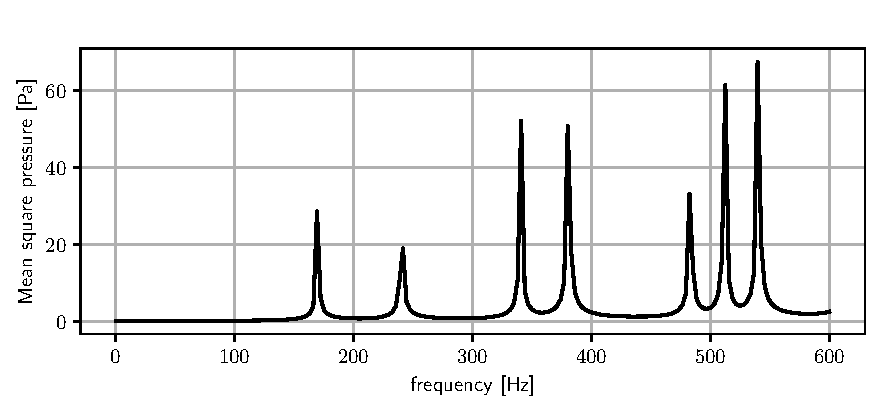
\includegraphics[width=0.9\textwidth]{pics/frf}
\caption{The frequency response plot shows the eigenfrequencies of the fluid in the domain. Exciting the fluid with an eigenfrequency leads to a comparatively strong response.}
\label{fig:frf}
\end{center}
\end{figure}







\chapter{Gaussian Processes and the Statistical Finite Element Method}
In this chapter, an introduction to Gaussian Processes and, building on it, statFEM is given. 

\paragraph{Literature Review} Regarding Gaussian Processes and the underlying probability theory, \cite{murphy2012} is a comprehensive and modern reference to get a good overview of the subject. It is an especially good choice to read for learning about probability theory and Bayesian Inference. The subject of kernels is described in much detail, also because it is an important building block in the big field of Machine Learning and not only GPs. For a thorough explanation of GPs themselves, \cite{rasmussen2006} is the best choice and the standard reference on the subject. statFEM was first introduced in \cite{girolami2021}. \cite{Duffin2020} modifies statFEM to work in a time-dependent context and provides a detailed mathematical derivation of the method. A first practical application is documented in \cite{Febrianto2021}: Sensor data from a railway bridge is fused with an FEM model of the bridge. Besides GPs, statFEM builds up upon the statistical generating model derived in \cite{kennedy2001}. statFEM focuses on finding an approximation of the model error, opposed to the well-established stochastic FEM \cite{Stefanou2009} which focuses on propagating uncertainty in the PDE parameters through a discretized model. A recently developed method to improve the capabilities of the FEM as a prior in Bayesian inversion, in the context of the stochastic FEM, is presented in \cite{Abdulle2021}. 
Another approach on approximating a posterior by providing a prior and conditioning it on measurements, hence very similar to statFEM, can be found in the area of model order reduction: Gappy POD, or Gappy proper orthogonal decomposition, first derived in \cite{Everson1995} and well explained in \cite{StevenL.Brunton2019}, is an adaptation of the well known Karhunen-Loeve transform. \cite{Rao2001} \cite{Loeve1994}

\section{Basic Probability Theory}
The statistical Finite Element Method (statFEM) is based on Gaussian Processes (GPs) and Bayesian inference. To be able to work with both, some basic understanding of probability theory is necessary.


\subsection{Random Variables and Distributions}
\label{sec:MultiGauss}
speak about linearity somewhere! see Römer lectures

explain PDF/CDF and moments

A random variable $X$ is considered normally, or Gaussian, distributed if $X \sim \mathcal{N}(\mu, \sigma)$ with $\mu$ the mean and $\sigma$ the standard deviation. The shape of the PDF is a Bell curve.

From any distribution, the moments of the random variable can be deduced. Using the PDF there holds for the mean
\begin{equation}
\mu = \mathbb{E}[X] = \int_{\mathbb{R}} x f_X(x) \, \mathrm{d}x
\end{equation}
%
and for the variance
\begin{equation}
\mathbb{V}[X] = \mathbb{E}[(X-\mathbb{E}[X])^2] = \mathbb{E}[X^2] - \mathbb{E}[X]^2 \;.
\end{equation}
%
For the covariance between two random variables $X$ and $Y$ there holds (see \cite[p. 1434]{arens2015})
\begin{equation}
\mathrm{cov}[X,Y] = \mathbb{E}[(X-\mathbb{E}[X])(Y-\mathbb{E}[Y])] = \mathbb{E}[XY] - \mathbb{E}[X] \mathbb{E}[Y]\;.
\label{eqn:Covariance}
\end{equation}
It is clearly visible that $\mathrm{cov}[X,X] = \mathbb{V}[X]$.
%
For the PDF of the Gaussian distribution there holds
\begin{equation}
f_X(x) = \frac{1}{\sigma \sqrt{2 \pi}} \exp(-\frac{1}{2} \left(\frac{x-\mu}{\sigma}\right)^2) \;.
\end{equation}
%
If multiple random variables are observed, which are all normally distributed, they can be aggregated in a so-called multivariate Gaussian disribution. Instead of a random variable it is a random vector which is defined by a mean vector and a covariance matrix. The matrix is named covariance and not variance matrix because not only the variance of the individual random variables but also the covariance among the different variables makes up entries of it. It is similar to auto- and cross correlation, both described in a single matrix.
For the PDF of a multivariate Gaussian distribution there holds
\begin{equation}
f_X(\bm{x}) = \frac{\exp(-\frac{1}{2}(\bm{x}-\bm{\mu})^T \Sigma^{-1}(\bm{x}-\bm{\mu}))}{\sqrt{(2\pi)^k \lvert \Sigma \rvert}}
\label{eqn:MultivariateGaussian}
\end{equation}
with $\Sigma$ the covariance matrix, $\bm{\mu}$ the mean vector and $k$ the dimension, i.e. the number of random variables, of the distribution.
An example of a multivariate Gaussian is visible in Figure \ref{fig:MultiGauss}. The underlying mean vector and covariance matrix read
\begin{equation}
\bm{\mu} = \begin{bmatrix}
           0 \\
           1
         \end{bmatrix}
, \quad     
\Sigma = \begin{bmatrix}
1 & -0.7 \\
-0.7 & 1.5 
\end{bmatrix} \;.
\end{equation}
The smaller the absolute of the non-diagonal entries of the covariance matrix is, the less correlated the individual variables are.

\begin{figure}[!ht]
\begin{center}
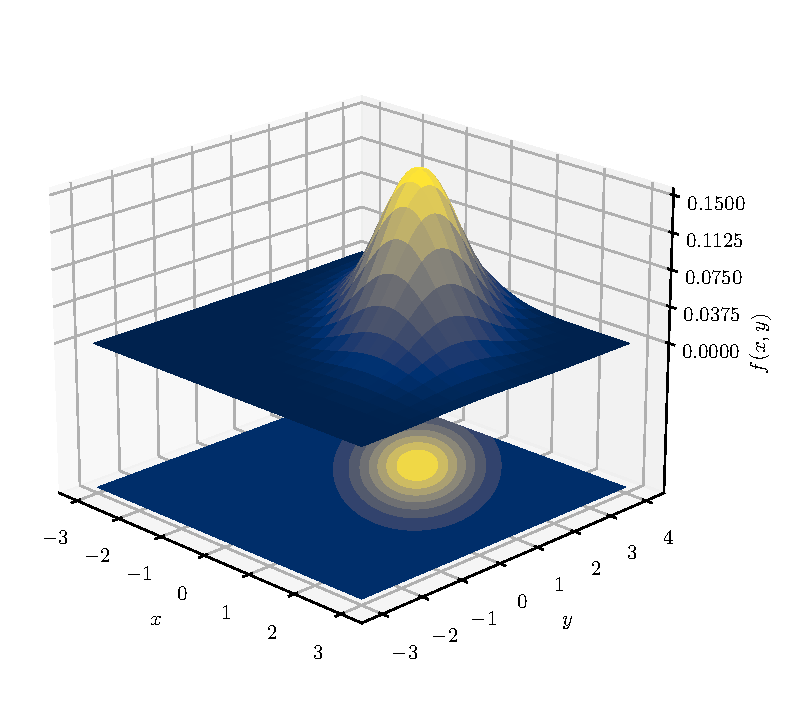
\includegraphics[width=0.6\textwidth]{pics/Gaussians}
\caption{A multivariate Gaussian distribution with two dimensions. A strong correlation between the two random variables is visible: No correlation would mean a perfect circle in the lower 2D plot. The more correlated the two dimensions are, the more elliptical the plotted PDF becomes. \cite{Virtanen2020} }
\label{fig:MultiGauss}
\end{center}
\end{figure}

\subsection{Bayesian Inference}
$posterior = \frac{likelihood x prior}{marginal likelihood}$ \cite{rasmussen2006}
explain basics of bayesian inference with bayes rule etc. what is posterior/prior 
explain what the marginal likelihood is

Bayesian Inference uses Bayes' law to infer a posterior density from a prior distribution and data. The data "updates" the prior. The law states that
\begin{equation}
p(\bm{u}|\bm{y}) = \frac{p(\bm{y}|\bm{u})p(\bm{u})}{p(\bm{y})}
\end{equation}
where $p(\bm{u}|\bm{y})$ is the posterior, $p(\bm{y})$ is the likelihood, $p(\bm{u})$ is the prior and $p(\bm{y})$ is the marginal likelihood, also called evidence. The posterior to be infered is the new probability density describing the sought quantity after observing data $y$. The data, i.e. measurements, aid understanding the problem what leads to a smaller variance in the posterior as comapared to the prior. The prior density describes the prior belief of the underlying process. It can be deduced from expert knowledge or from previous measurement. 
The likelihood describes the probability of the data to be measuered at all given that, in the case of this thesis, the FEM solution holds: "How likely is the measured data to be true, according to the model?"
The marginal likelihood (see section \ref{sec:Marg} for more detail) serves as a normalization constant and describes how likely it is to measure the observed data.


\section{Gaussian Process Regression}
statFEM is based on Gaussian Processes (GPs), a method known from Machine Learning. \cite{murphy2012} GPs can be used for regression, i.e. to find a suitable function which describes a given set of points as good as possible, but also for classification and clustering. \cite{gortler2019} 
Gaussian Processes are a class of Bayesian non-parametric models. Non-parametric doesn't mean that there are no parameters involved but rather that there is an infinite number of them. \cite{gortler2019} Every realization of a Gaussian process doesn't yield a scalar or vector but a function. One can think of a Gaussian Process as a collection of infinitely many normally distributed random variables, i.e. a generalization of a Gaussian distribution: A vector with infinitely many entries is basically a function. By picking out a finite set of those random variables when discretizing e.g. on an FEM mesh, one obtains a multivariate distribution which is determined by a mean and a covariance matrix. \cite[p. 2]{rasmussen2006} Hence, GPs are a method to obtain a distribution over functions: Around a mean function a variance is defined. Possible samples from the GP are functions within these confidence bands. In statFEM, the FEM prior and also the solution are modeled as GPs. This provides an elegant way to incorporate uncertain data in an FEM solution to eventually improve it. To understand how that works, the general idea of regression and the mathematical basis of GPs have to be explained.
\subsection{Linear Regression}
Following \cite{murphy2012}, regression, in most cases linear regression, is a parametric model. This means that there are certain parameters involved in a model which can be changed to match given data as closely as possible regarding some measure of accuracy. A regression is linear if the output of a function depends linearly on its inputs, as in (\ref{eqn:linReg}). \cite[p. 19]{murphy2012}
%
\begin{equation}
y(\bm{x}) = \bm{w}^T \bm{x} + \epsilon = \sum_{j = 1}^D w_jx_j + \epsilon
\label{eqn:linReg}
\end{equation}
%
$\bm{x}$ is the input vector, $\bm{w}$ the corresponding vector of input weights and $\epsilon$ is the error between the output of the regression and the true, measured values. The error term is usually modeled as a Gaussian $\epsilon \sim \mathcal{N}(\mu,\sigma^2)$ with zero mean $\mu = 0$ and some defined variance. Because of the addad Gaussian, every solution in the solution space of the function is now not only a scalar but a normally distributed random variable. Therefore, the whole function can be expressed as a probability density:
%
\begin{equation}
p(y|\bm{x},\bm{\theta}) = \mathcal{N}(y|\mu(\bm{x}),\sigma^2(\bm{x}))
\end{equation}
%
Note that the mean $\mu(\bm{x})$ now depends on the input vector. For a linear approximation there holds
\begin{equation}
\mu (\bm{x}) = w_0 + w_1x= \bm{w}^T\bm{x} \;.
\end{equation}
Unintuitively, using basis function expansion, linear regression can be used to model a non-linear behaviour. If polynomials are used as basis functions, one speaks of polynomial regression. The probability density would read
\begin{equation}
p(y|\bm{x},\bm{\theta}) = \mathcal{N}(y|\bm{w}^T\Phi(\bm{x}),\sigma^2(\bm{x}))
\end{equation}
with 
\begin{equation}
\Phi(\bm{x}) = [1,x,x^2,x^3,...,x^d]
\end{equation}
where the complexity of the approximation rises with $d$. \cite[p. 20]{murphy2012}
The model now has to be fit to given data, i.e. the input weight vector has to be defined. This works, for example, by using a maximum likelihood estimation (MLE), also called least squares.




"Regression is used to find a function that rerpesents a set of data points as closely as possible" \cite{gortler2019}
\cite{gortler2019} "A Gaussian process is a probabilistic method that gives confidence for the predicted function"

"GPs allow us to make predictions about our data incorporating prior knowledge"



The following closely follows \cite{rasmussen2006}.




A GP is described by its mean function and the covariance function, also called kernel.






\subsection{Gaussian Processes}

Gaussian Process regression is another type of regression but ultimately has the same goal as, for instance, a polynomial regression. The difference is that a GP isn't constrained to a parametric model, i.e. it is more flexible. (And therefore prone to overfitting! Really? Check that.) Instead of using a polynomial or some other equation as a basis function, GPs utilize a kernel function which is able to output an infinite amount of different functions. More on kernels later.
A GP is more flexible than a standard linear or polynomial regression: A GP regressor finds a suitable function out of infinitely many possible functions. For a linear regression, the function type and therefore basis functions need to be known beforehand in order to achieve accurate results. For a problem of which the function shape cannot be determined beforehand, GPs yield the better results. See an example in Figure \ref{fig:GPvsReg}. For both plots the same polynomial regressor and GP were used.
\begin{figure}[!ht]
\begin{center}
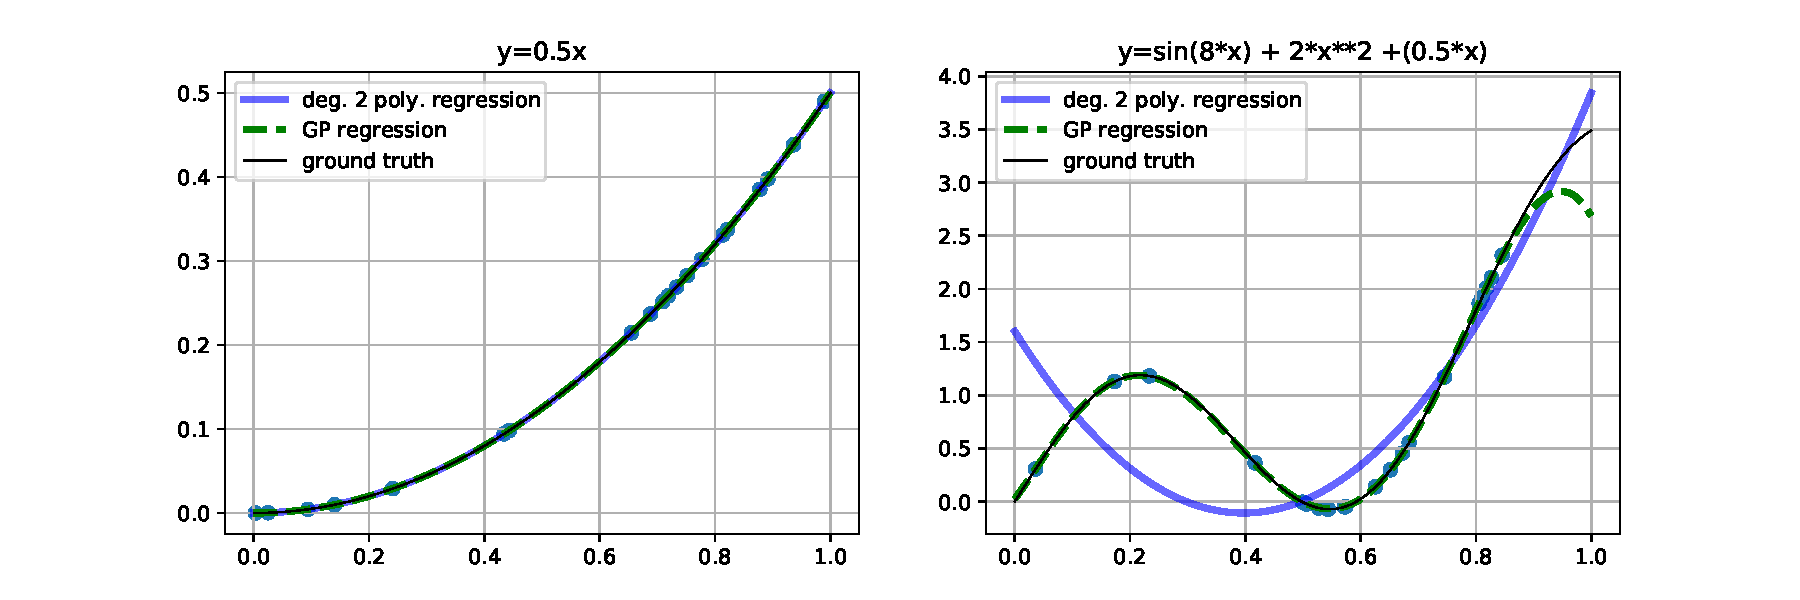
\includegraphics[width=1.1\textwidth]{pics/GPvsReg}
\caption{On the left: Regression for a 2nd degree polynomial. Both linear regression and GP approximate it fine. On the right: The same GP as on the left is able to model the ground truth accurately, the polynomial regression does not. The GP behaves more flexible in this case.}
\label{fig:GPvsReg}
\end{center}
\end{figure}
GPs are non-parametric: This means that, as opposed to standard linear regression where parameters are optimised, a GP does not have a certain number of parameters. Rather, the number of parameters depends on the number of test and training points and could in theory be ininitely large. \cite{murphy2012} 
GPs are constructed using multivariate Gaussians which were explained in Section \ref{sec:MultiGauss}. Also, as mentioned before, they represent a distribution over functions: The term "process" refers to the generalization from a Gaussian random variable to a random function. \cite[p.13]{rasmussen2006}  The relationship between multivariate Gaussians and functions will be explained following \cite{damianou2021}.

The simplest GP is a bivariate Gaussian. For each of the two random variables, i.e. dimensions, a mean and a variance are defined. Also, the covariance between both random variables is given. Now, samples can be drawn from each random variable. As an example see Figure \ref{fig:bivarGP}. In the lower half of the plot the samples are visible in the already described 2D plane. The upper half shows the individual samples compared to each other. Drawing samples from a bivariate Gaussian leads to different results depending on the correlation between the two random variables. The more correlated they are, the smaller the difference between the sampled values in each dimension.
%
\begin{figure}[!ht]
\begin{center}
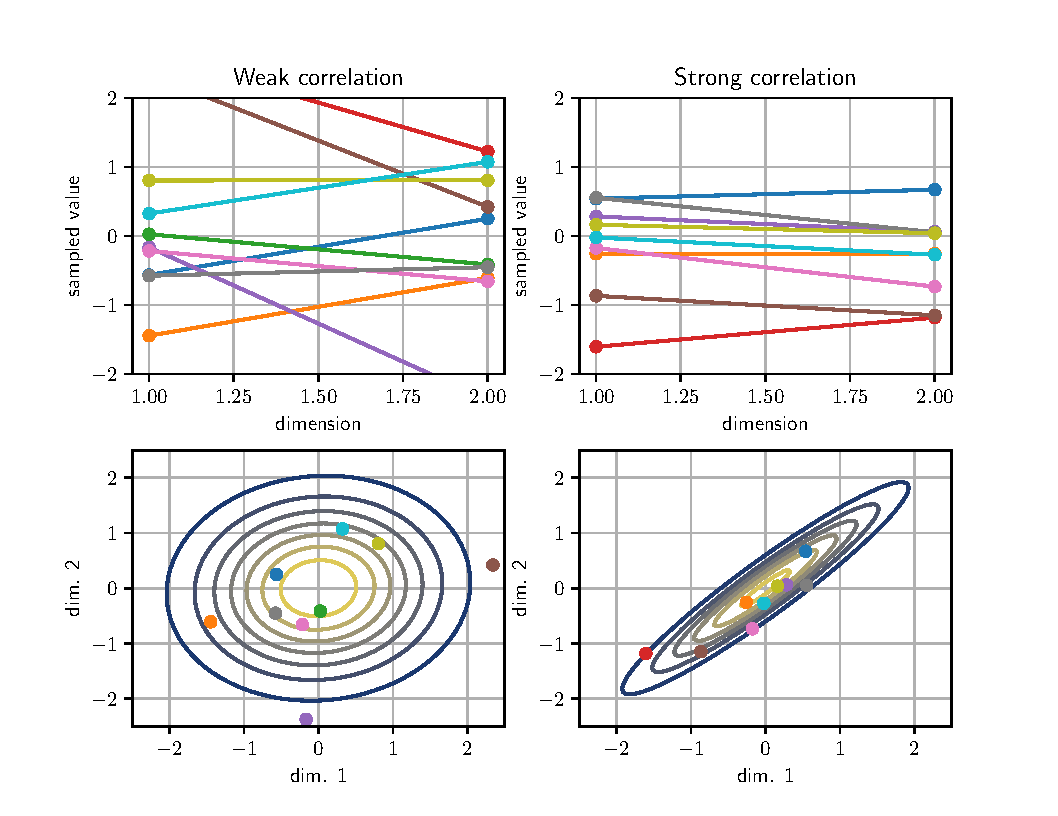
\includegraphics[width=1\textwidth]{pics/bivarGP}
\caption{A bivariate Gaussian can be interpreted as a GP. The more corellated the random variables are, the closer together the sampled values are. The plots on the top show the samples drawn from the well-known 2D PDF in another way: Sampling from a multivariate Gaussian yields a vector of correlated samples which can be interpreted as a subset of an infinitely dimensional vector, i.e. a function.}
\label{fig:bivarGP}
\end{center}
\end{figure}
%
Of course, this also holds true for multivariate Gaussians with even more random variables, as visible in Figure \ref{fig:multiGP}.
\begin{figure}[!ht]
\begin{center}
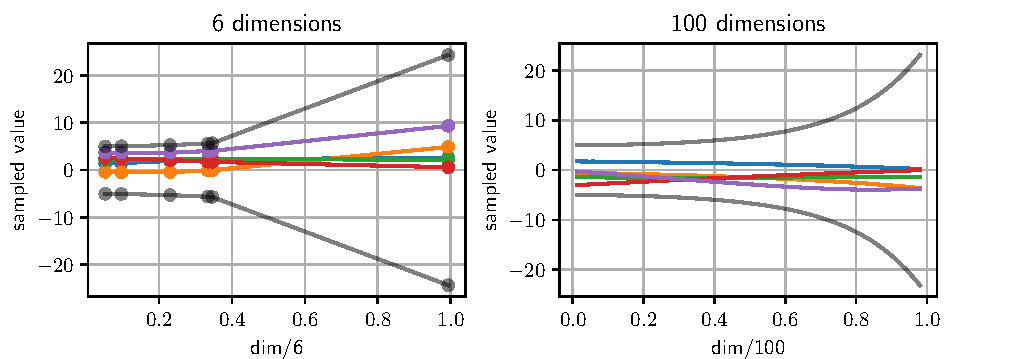
\includegraphics[width=1\textwidth]{pics/multivarGP}
\caption{The more random variables are used to construct the multivariate Gaussian, the more the result looks like a smooth function. Since each variable is a random variable, there is also a variance available for every dimension, visible in grey.}
\label{fig:multiGP}
\end{center}
\end{figure}
%
In theory, a GP can consist of infinitely many correlated random variables and a vector with infinitely many entries is basically a function. Therefore every sample of a GP is a function and also the variance is given as a function. Drawing samples from a GP can be imagined as drawing correlated samples from a large set of random variables. However, a GP is, at first, defined continuously: To construct a GP, a mean function and a covariance function have to be given. The mean function can be any function, but the covariance function, also called kernel, has to obey certain rules. More on that later.  Nevertheless, to use Bayesian inference, i.e. to form a posterior distribution over functions, the continuous GP has to be represented as a multivariate Gaussian, i.e. discretely, again. To understand how and why this is done, the concepts of marginalization and conditioning have to be explained at first.

\paragraph{Marginalization and Conditioning} 
\label{sec:Marg}
Marginalisation means that out of a multivariate Gaussian the single variables can directly be taken out of the mean vector and the covariance matrix. E.g. for a point on the axis described by the GP, a single value can be picked out. A univariate Gaussian comes out by simply using the mean vectors value at that point and the i,i th index of the covariance matrix. This means that the underlying distributions for single variables do not change if a GP is used to describe an arbitrary set of variables [p13].
[Visual Exploration]
From a multivariate, in this case bivariate, Gaussian
\begin{equation}
P(X,Y) = \begin{bmatrix}
           X \\
           Y
         \end{bmatrix} \sim \mathcal{N}\left( \begin{bmatrix}
           \mu_X \\
           \mu_Y
         \end{bmatrix}, \begin{bmatrix}
\Sigma_{XX} & \Sigma_{XY} \\
\Sigma_{YX} & \Sigma_{YY} 
\end{bmatrix}  \right)
\end{equation}
one single random variable, say $X$, can be marginalised out by simply only looking at the entries corresponding solely to $X$:
\begin{equation}
X \sim \mathcal{N}(\mu_X, \Sigma_{XX}) \;.
\end{equation}
If the covariance matrix and mean vector are not known, a random variable can be marginalised out of an arbitrary distribution by
\begin{equation}
p_X(x) = \int_y p_{X,Y}(x,y)\,\mathrm{d}y = \int_y p_{X|Y}(x|y)p_Y(y)\,\mathrm{d}y
\label{eqn:margi}
\end{equation}
which intuitively means that summing the probability for $X$ at every possible $Y$ gives the total probability for $X$ independent of $Y$. 

(\ref{eqn:margi}) already uses the principle of conditioning. The condition operator $|$ yields the probability of one variable under the condition that another variable is true. As an illustration in words one could ask: "What is the probability of event $X$ to happen under the condition, that the event $Y=y$ happens simultaneously?"
For the multivariate Gaussian there holds for the conditioning
\begin{equation}
X|Y \sim \mathcal{N}(\mu_X +\Sigma_{XY} \Sigma_{YY}^{-1}(Y-\mu_Y), \Sigma_{XX} - \Sigma_{XY}\Sigma_{YY}^{-1}\Sigma_{YX} ) \;.
\end{equation}
%
Conditioning yields a so-called modified Gaussian distribution which can be imagined as a "cut" through a multivariate Gaussian $P(X,Y)$ at a certain point $y$. A new Gaussian with the dimension reduced by $1$ arises as illustrated in Figure \ref{fig:GaussCut3d}.

%
%
\begin{figure}[!ht]
\begin{center}
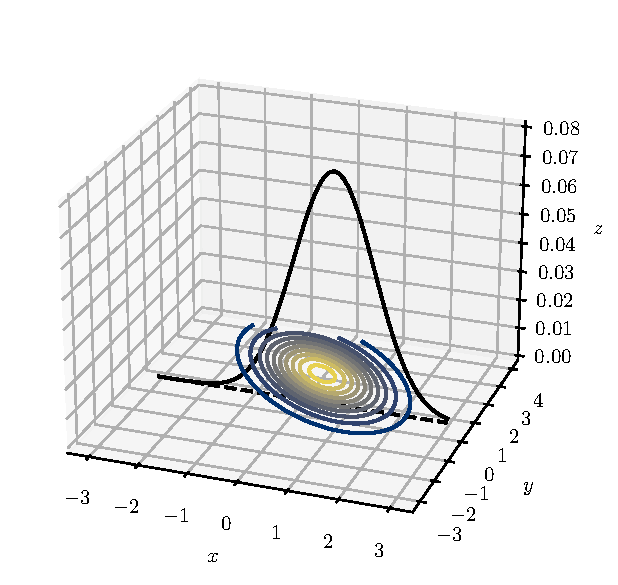
\includegraphics[width=0.6\textwidth]{pics/Gaussians3dCut}
\caption{Cutting, i.e. conditioning, a bivariate Gaussian leads to a new Gaussian with only one dimension. This example shows the result for a cut at the dashed line. The new Gaussian has a new mean and variance.}
\label{fig:GaussCut3d}
\end{center}
\end{figure}



\subsection{Kernel Functions}

Kernel functions have already been mentioned before. They are what makes a GP regression different from a standard linear regression approach: A kernel function allows to not form a distribution over parameters of some predefined function but rather over the output functions themselves. This means that no assumptions for the shape of the approximated function have to be made. For example, a polynomial could be resembled by a kernel function which is not defined using any polynomial. The same kernel function can be used to resemble a sine wave or anything else. If linear regression is used, there needs to be much more prior knowledge about the shape of the underlying function of the observed data to make accurate predictions: Approximating a sine wave needs periodical basis functions and approximating polynomials of a certain degree needs polynomial basis functions of at least that degree.

A kernel $k$ is a function which takes two points $x \in \mathbb{R}^n$ and $x' \in \mathbb{R}^n$ and maps them into $\mathbb{R}$ \cite[p.80]{rasmussen2006}, i.e. it returns a scalar which serves as a similarity measure between the two points \cite{gortler2019}:
%
\begin{equation}
k: \mathbb{R}^n \times \mathbb{R}^n \mapsto \mathbb{R}, \quad \Sigma = \mathrm{Cov}(X,X') = k(x,x') \;.
\end{equation}
%
If a kernel function is evaluated at a finite number of points, say all the test points, a covariance matrix $\Sigma$ is created. It can be used as the covariance of a multivariate Gaussian from which samples can be drawn. The values of each entry are a function over the input points of the kernel function and describe, how much the two points are correlated. \cite[p.14]{rasmussen2006}

In a covariance function all the assumptions of the function to be modeled are contained. The kernel defines or rather assesses how near or similar a value of one point is to the one of another. A training point which is close to a test point therefore gives information on how the value at the test point should be. \cite[p.79]{rasmussen2006}
A kernel function is usually symmetric ($k(x,x') = k(x',x)$) and greater than zero ($k(x,x') \geq 0$). \cite[p.481]{murphy2012}
Free parameters inside a kernel function are called hyperparameters. The term 'hyper' states that they are not parameters of the model itself but only of the kernel which defines properties of the model.

\paragraph{Stationarity}
Kernels which are a function of $x-x'$ are called \emph{stationary} kernels. They are stationary because it doesn't matter what value $x$ and $x'$ have as a starting value, the difference is always the same. Example: $110\mathrm{Pa} -100\mathrm{Pa} = 10\mathrm{Pa}, 1010\mathrm{Pa}-1000\mathrm{Pa} = 10\mathrm{Pa}$.
%
A radial basis function is a function which is only a function of $r=x-x'$ and which is therefore isotropic, i.e. there are no rigid motions. r is like a radius so these functions are called radial basis functions. \cite[p.80]{rasmussen2006} 
Covariance matrices always have to be symmetric, i.e. $k(x-x') = k(x'-x)$ because $x-x'$ is a distance measure.
The so-called Gram matrix is the function containing $x-x'$ evaluated at a set of points $x_i$. If the function is a covariance funtion, the gram matrix is called covariance matrix.


\paragraph{Positive Definiteness} A covariance function has to be positive semidefinite, i.e. all eigenvalues are greater or equal zero. A covariance matrix K is positive semidefinite when $Q(v) = v^T K v \geq 0$. Q is the quadratic form. A kernel function is positive semidefinite if it only outputs matrices which are positive semidefinite.


\paragraph{The Characteristic Length Scale} The number of "upcrossings" in the interval, i.e. the number of crossings of the x axis can be thought of as the characteristic length scale of the kernel function. It can be calculated with \cite[Eq. 4.3]{rasmussen2006}. The more upcrossings, the shorter the length scale and the more jagged the function looks. Long length scales lead to rather smooth looking functions.

A comprehensive overview of different kernel functions and their behavior is given in \cite{Duvenaud} and \cite{gortler2019}. Nevertheless, some important kernels will be introduced below.
%

\paragraph{Linear Kernel Functions}
A general linear kernel is defined as
\begin{equation}
\sigma_b^2 + \sigma^2 (x-c) (x'-c) \;.
\end{equation}
As the name suggests, samples drawn from a GP with a linear kernel are linear functions. The paramter $c$ controls the point which all samples pass. Depending on the added noise, the variance around that point is much lower as in the other intervals. Figure \ref{fig:Linear} shows exemplaric samples. Different to the other kernels introduced here, the linear kernel is non-stationary, i.e. the absolute position of the two inputs matters.
\begin{figure}[!ht]
\begin{center}
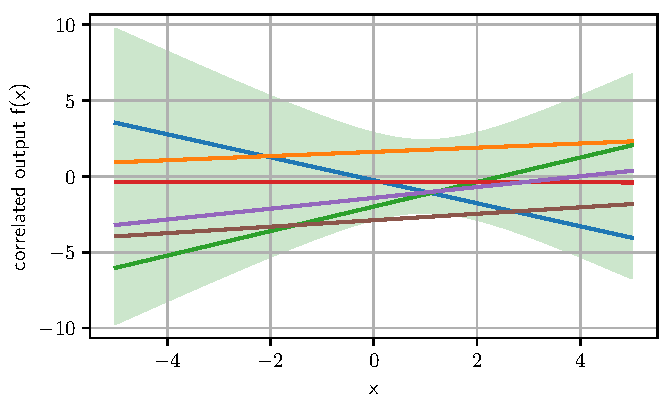
\includegraphics[width=0.6\textwidth]{pics/LinearKernel.pdf}
\caption{Samples drawn from a GP with a linear covariance function. There is a region with relatively low variance through which all samples pass. The poosition can be mived by varying a hyperparameter of the kernel.}
\label{fig:Linear}
\end{center}
\end{figure}



\paragraph{Squared Exponential Kernel Functions}
The squared exponential kernel function is the most commonly used kernel function for GPs. It is stationary and infinitely differentiable, hence very smooth. A GP with this kernel function is the same as the above discussed linear regression model with infinitely many basis functions. \cite{rasmussen2006} This makes clear, why GPs are considered non-parametric models. Not the parameters are optimized but the function itself. It wouldn't be possible to learn an infinite amount of parameters.
It is defined as
\begin{equation}
k_{SE} = \sigma \exp(-\frac{r^2}{2l^2})
\end{equation}
%
and can be defined as a Python function with
\begin{python}
def squared_exponential(xa, xb, l, sig):
    sq_norm = -0.5 * scipy.spatial.distance.cdist(xa, xb, 'sqeuclidean') \
    	* (1/l**2)
    return sig**2 * np.exp(sq_norm) .
\end{python}
\label{lst:sqEx}
\cite{murphy2012}

\begin{figure}[!ht]
\begin{center}

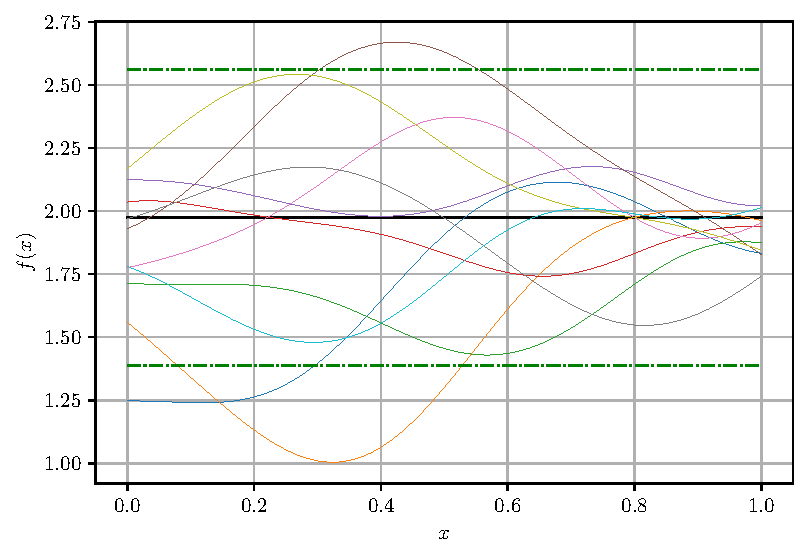
\includegraphics[width=0.6\textwidth]{pics/sqexp_f_sampled}
\caption{The source term GP of $f(x)$ sampled for a Squared Exponential kernel with $l = 0.25$ and $\sigma = 0.3$. $\bar{f}(x)$ in solid black, $2\sigma$ confidence bands in green. The samples are very smooth, which is a charcteristic of this particular kernel.}
\label{fig:Matern1_2}

\end{center}
\end{figure}

\paragraph{Periodic Kernel Functions}
The periodic kernel is defined as
\begin{equation}
\sigma^2 \exp(- \frac{2 \sin^2 (\pi r /p)}{l^2}) \;.
\end{equation}
The parameter $p$ defines the periodicity, i.e. the higher $p$, the larger the period.  $\sigma$ and $l$ have the same function as in the squared exponential kernel. \cite{Duvenaud}
It can be used if a periodic behavior in the modeled process is expected. Figure \ref{fig:CovMats} shows an example of the generated covariance matrix. The periodicity is visible as a periodic high correlation between the dimensions. Figure \ref{fig:Periodic} shows three exemplaric samples from a GP with zero mean and a periodic kernel.
\begin{figure}[!ht]
\begin{center}
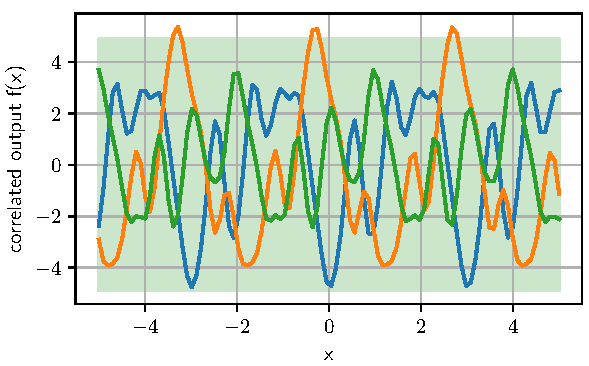
\includegraphics[width=0.6\textwidth]{pics/PeriodicKernel.pdf}
\caption{Three samples from a periodic kernel. The periodicity is clearly discernible. The variance is constant.}
\label{fig:Periodic}
\end{center}
\end{figure}



\paragraph{Dirichlet Kernel Functions}


\paragraph{Matern Kernel Functions}
\cite{rasmussen2006} The squared exponential kernel is infinitely differentiable, which means that it behaves very smoothly. This is considered as unphysical by \cite{stein1999}. Therefore, the Matern class of covariance functions \cite{matern2013} is recommended by \cite{stein1999} which is finitely differentiable and therefore less smooth. It is called a "class" of kernels because by varying the parameters, very different behaviours can be obtained. The squared exponential kernel is actually a special case of the Matern class.

The general Matern kernel is defined as
\begin{equation}
k_M(r) = \sigma^2 \frac{2^{1-\nu}}{\Gamma(\nu)}  \left( \frac{\sqrt{2\nu}r}{l}  \right)^{\nu} K_{\nu}  \left(  \frac{\sqrt{2\nu}r}{l}   \right)
\label{eqn:MaternKernel}
\end{equation}
with $\Gamma(\nu) = (\nu - 1)!$ the gamma function and $K_{\nu}$ a modified Bessel function \cite[p.84 ff.]{abramowitz2013}, \cite{rasmussen2006}. $\nu$ and $l$ are free positive parameters.
For $\nu \to \infty$  (\ref{eqn:MaternKernel}) becomes the squared exponential kernel.
The covariance function simplifies for half integer values of $\nu$ and can be expressed as a product of an exponential and a polynomial. According to \cite{rasmussen2006} $\nu = 3/2$ and $\nu = 5/2$ are commonly used for GPs; the simplest Matern kernel is obtained with $\nu = 1/2$:

\begin{align}
k_{M;\nu = 1/2}(r) &=   \sigma^2 \exp(- \frac{r}{l})  \; , \\
\label{eqn:Materns1}
k_{M;\nu = 3/2}(r) &=  \sigma^2 \left(      1+ \frac{\sqrt{3}r}{l}  	\right)  \exp(- \frac{\sqrt{3} r}{l})  \; , \\
k_{M;\nu = 5/2}(r) &=  \sigma^2\left(      1+ \frac{\sqrt{5}r}{l}  + \frac{5r^2}{3l^2}	\right)  \exp(- \frac{\sqrt{5} r}{l}) \; .
\label{eqn:Materns3}
\end{align}
%
(\ref{eqn:Materns1}) - (\ref{eqn:Materns3}) are used in this thesis. Figures \ref{fig:Matern1_2} - \ref{fig:Matern5_2} show the differences between the different choices for $\nu$: The higher it is chosen, the smoother the GP becomes and the closer it gets to the squared exponential kernel.
\begin{figure}[!ht]
\begin{center}

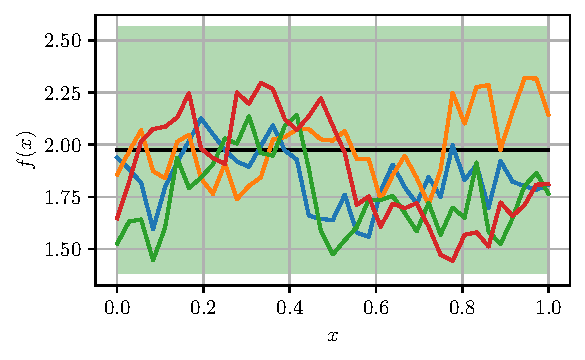
\includegraphics[width=0.6\textwidth]{pics/matern1_2_f_sampled}
\caption{The source term GP of $f(x)$ sampled for a Matern kernel with $\nu=1/2$. $\bar{f}(x)$ in solid black, $2\sigma$ confidence bands in green. For this $\nu$ the samples behave very rough.}
\label{fig:Matern1_2}

\end{center}
\end{figure}

\begin{figure}[!ht]
\begin{center}

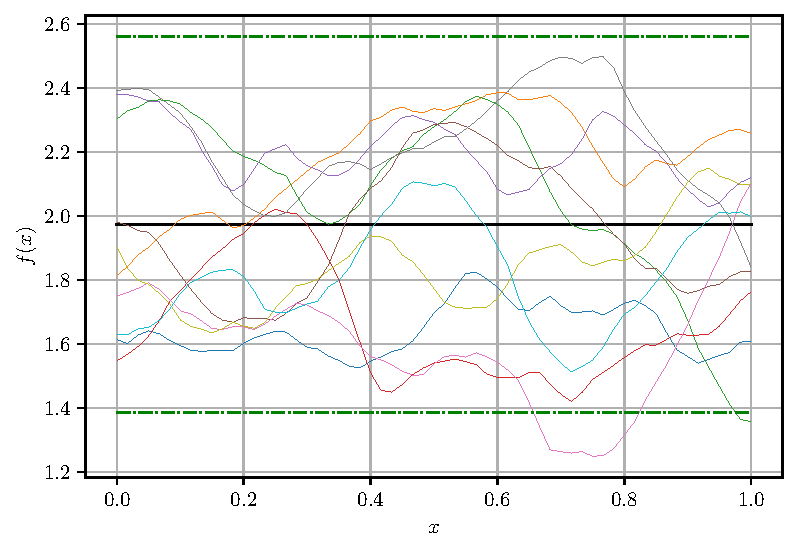
\includegraphics[width=0.6\textwidth]{pics/matern3_2_f_sampled}
\caption{The source term GP of $f(x)$ sampled for a Matern kernel with $\nu=3/2$. $\bar{f}(x)$ in solid black, $2\sigma$ confidence bands in green. For this $\nu$ the samples behave less rough.}
\label{fig:Matern3_2}

\end{center}
\end{figure}

\begin{figure}[!ht]
\begin{center}

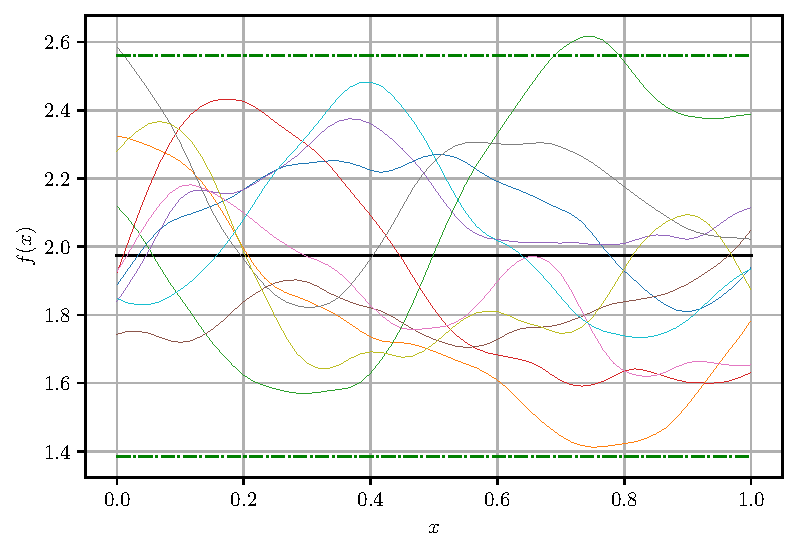
\includegraphics[width=0.6\textwidth]{pics/matern5_2_f_sampled}
\caption{The source term GP of $f(x)$ sampled for a Matern kernel with $\nu=5/2$. $\bar{f}(x)$ in solid black, $2\sigma$ confidence bands in green. For this $\nu$ the samples behave almost as smooth as in the Squared Exponential kernel.}
\label{fig:Matern5_2}

\end{center}
\end{figure}




\begin{figure}[!ht]
\begin{center}
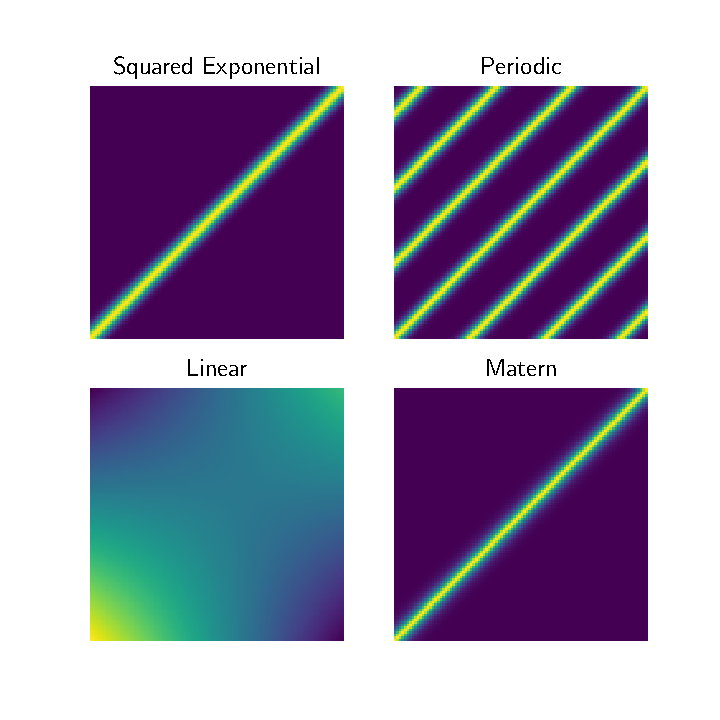
\includegraphics[width=0.6\textwidth]{pics/CovMats.pdf}
\caption{The covariance matrices for the different kernel functions. 100 linearly spaced test points between $-5$ and $5$ were used as inputs. The Squared Exponential and Matern kernels yield similar results. For the periodic kernel, the periodicity is also visible in the covariance matrix. For the covariance matrix derived from the linear kernel, the region of lower variance is visible.}
\label{fig:CovMats}
\end{center}
\end{figure}



\paragraph{Combination of Different Kernel Functions}
Different kernels can now easily be combined by adding or multiplying individual functions. For example, a periodic kernel can be superimposed on a linear kernel by addition which would lead to a periodic kernel with a mean that changes linearly. Multiplying two linear kernels leads to sampled functions which are quadratic. Multiplying across dimensions, i.e. for example
\begin{equation}
k_{new}(x,y,x',y') = k_x(x,x')k_y(y,y') \;,
\end{equation}
yields functions in which the function values are correlated on two axes. \cite{Duvenaud}

\subsection{Bayesian Inference}
Now that the mathematical prerequisites have been discussed, the actual Bayesian Inference with GPs can be explained. The goal is condition a prior GP on observed data. This means that the variance over the mean function in a GP should become lower at positions where measurements have been taken, since at these locations the value of the measured quantity is known accurately. Also, the mean function will change to that now well known value. At first, knowledge of the measured quantity is collected as information within the Bayesian prior.
\paragraph{Prior}
In a differential equation, such as the ones used in this thesis, one or more spatial parameters or the source term can be considered as random. Assuming a probability distribution for these parameters according to already given knowledge about and solving the PDE leads to the so called prior. The prior, because it is modeled as random, already involves a mean and a covariance for the parameters. Constructing the prior as a GP already at this point is a useful approach to make the further steps easier, since a covariance matrix and a mean function are already known, which are later used for inference. Therefore, the mean and covariance of the random parameters are constructed as mean and covariance \emph{functions} within the framework of a GP, which in turn yields a prior distribution over functions. To obtain the covariance matrix, a kernel function suitable to the problem has to be chosen. At this point, the hyperparameters are chosen manually according to prior belief and knowledge: They can for example be adjusted to make the function behave more smoothly or to change the confidence bands in which possible functions may appear. Then, evaluating the kernel function at a set of test points, which could for instance be the nodes in an FEM mesh, leads to the covariance matrix. The mean vector is chosen manually, as well.
To visualise the prior, samples from it can be drawn.
The following closely follows \cite[A2]{rasmussen2006}.
To obtain a sample from the multivariate Gaussian which represents the GP, at first the Cholesky decomposition of the covariance matrix $\Sigma = LL^T$ has to be computed. Next, a sample from a standard multivariate normal distribution $\bm{u} \sim \mathcal{N} (\bm{0},\bm{I})$ is drawn. The final sample $\bm{x}$ can now be obtained using
\begin{equation}
\bm{x} = \bm{m} + L \bm{u} 
\end{equation}
with the prescribed mean vector $\bm{m}$.
With Python and numpy, the sample is obtained with
\begin{minted}
[
frame=lines,
framesep=2mm,
baselinestretch=1.2,
bgcolor=backcolour,
fontsize=\footnotesize,
linenos
]
{python}
x = np.random.multivariate_normal(
			mean = mean, cov=Sig,
			size=1)
\end{minted}
The numpy function does the Cholesky decomposition internally.
	
	
			
\paragraph{Occam's Razor}

\paragraph{Posterior after observation}
\label{sec:GPcond}
p16:
The prior is conditioned on the observations. It would also be possible, but computationally demanding, to sample many many functions out of the GP and only take those which go through the training points.

As observed data, also called training data, is available, the prior GP can be conditioned on those in order to compute a posterior distribution. If the observations are assumed to be noise-free, a joint distribution of the prior GP (here $X$) (with the kernel function evaluated at the chosen test points to form the covariance matrix) and the training data GP (here $Y$). The training data, even though noise-free, is a GP and therefore a multivariate Gaussian, because also here a covariance is formed by evaluating the kernel function at the sensor locations. The measured values form the mean vector. The joint density can be expressed as
%
\begin{equation}
P(X,Y) \sim \mathcal{N}(\bm{\mu},\Sigma) = \begin{bmatrix}
           X \\
           Y
         \end{bmatrix} \sim \mathcal{N}\left( \bm{\mu}, \begin{bmatrix}
K_{XX} & K_{XY} \\
K_{YX} & K_{YY} 
\end{bmatrix}  \right) \; .
\label{eqn:noisefreeJoint}
\end{equation}
The non-diagonal entries in \ref{eqn:noisefreeJoint} are formed by evaluating the kernel function with both the test and training points as arguments: For $r = x-x'$ there holds $r = \bm{x} - \bm{y}$ with $\bm{x}$ and $\bm{y}$ the vectors of the spatial coordinates for test and training points.
This density now has to be conditioned on the training data. This means that all samples from the new, conditioned, density will pass through the training points. This process can be thought of as sampling one function at a time from \ref{eqn:noisefreeJoint} and collecting all samples which pass through the training points, discarding all other ones. Of course, mathematically, this can be done using the already shown equations for conditioning densities, see Section \ref{sec:Marg}.

For noisy observations, i.e. there is an uncertainty in the measurement method, a diagonal noise term is added to the observation GP. For the joint distribution there now holds
\begin{equation}
P(X,Y) \sim \mathcal{N}(\bm{\mu},\Sigma) = \begin{bmatrix}
           X \\
           Y
         \end{bmatrix} \sim \mathcal{N}\left( \bm{\mu}, \begin{bmatrix}
K_{XX} & K_{XY} \\
K_{YX} & K_{YY} + \sigma_n^2 I 
\end{bmatrix}  \right)
\label{eqn:noiseJoint}
\end{equation}
with $\sigma_n^2$ the variance of an independent and identically distributed Gaussian noise and $I$ the identity matrix. Conditioning on $Y$ now yields
\begin{equation}
\begin{aligned}
X|Y \sim \mathcal{N}(\mu_X +K_{XY} [K_{YY}+ \sigma_n^2 I ]^{-1}(Y-\mu_Y), \\
K_{XX} - K_{XY}[K_{YY}+ \sigma_n^2 I ]^{-1}K_{YX} ) \;.
\end{aligned}
\label{eqn:ConditioningDistr}
\end{equation}
The conditioned distribution is a GP again: Conditioning therefore basically means interpolating between and extrapolating from the sensor locations. \cite{damianou2021}
%
%
Figure \ref{fig:GPExpl} shows both the GP prior and posterior. It is visible that the prior on the left has a zero mean. Arbitrarily many samples can be drawn from it which themselves do not necessarily have a zero mean, as well. If that prior GP is now conditioned on training points, two in this case, the mean of the newly formed GP will follow the training points and therefore deviate from the prior mean. All samples drawn from the posterior GP will go through the training points.  It is also visible, that the variance decreases in the surrounding of a measurement: Exactly on the (here noise-free) training points it is zero and in between them it is still much lower than the prior variance. Finding a new mean and variance between training points is called interpolation and, as visible, yields in solutions with relatively low variance. However, extrapolation yields results with higher variance: If only on one side of the domain a training point is available,the variance and the mean quickly become those of the prior again.
\begin{figure}[!ht]
\begin{center}

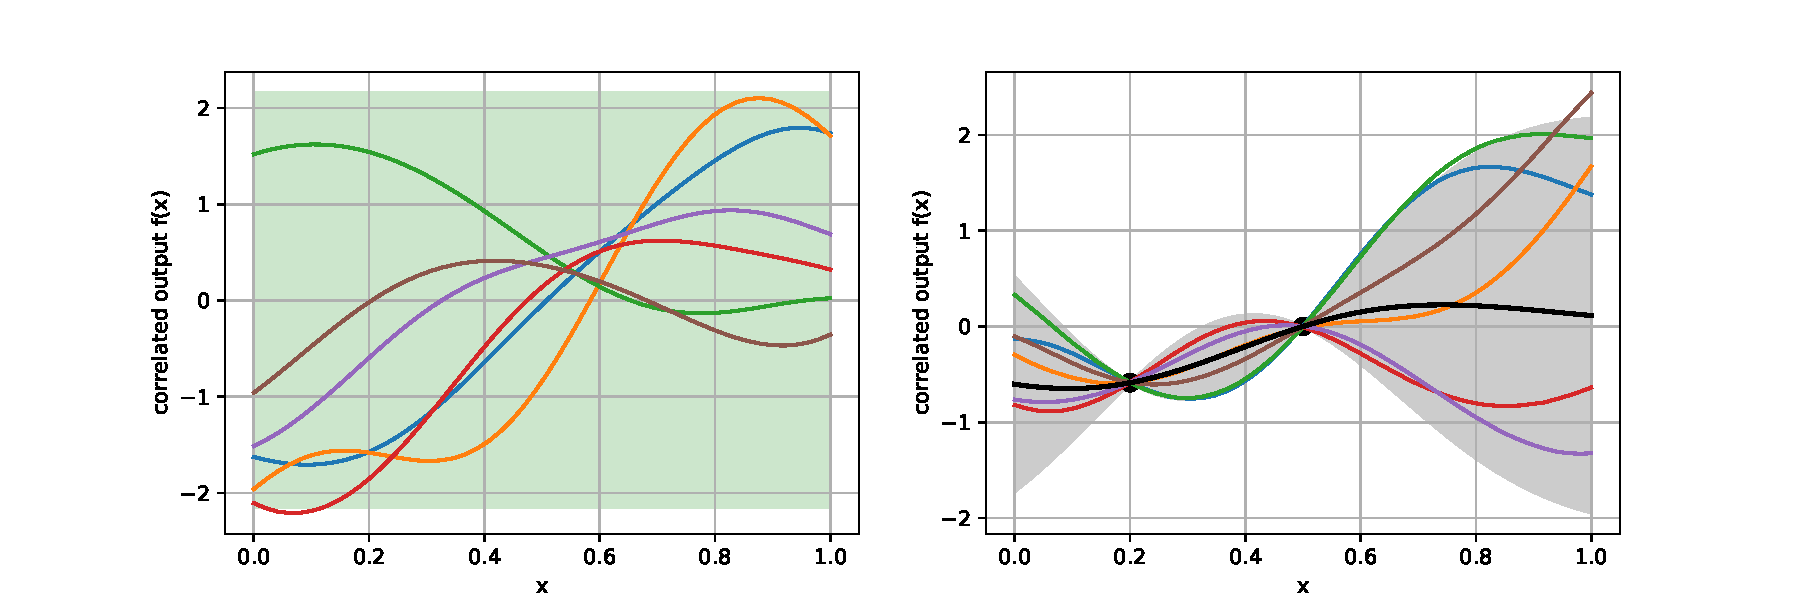
\includegraphics[width=1.1\textwidth]{pics/GPExpl}
\caption{The prior GP on the left and the posterior GP after conditioning on two training points on the right. The variance approaches zero at the noise-less training points. The further away from the training points, the closer the variance is back at the prior variance.}
\label{fig:GPExpl}

\end{center}
\end{figure}

Figure \ref{fig:CovPOst} shows the new covariance matrix after conditioning. It is visible that the variance is highest in the top right corner, which corresponds to values around $1.0$ and is in agreement with Figure \ref{fig:GPExpl}: The entries of the covariance matrix become lower in regions around a sensor location.

\begin{figure}[!ht]
\begin{center}

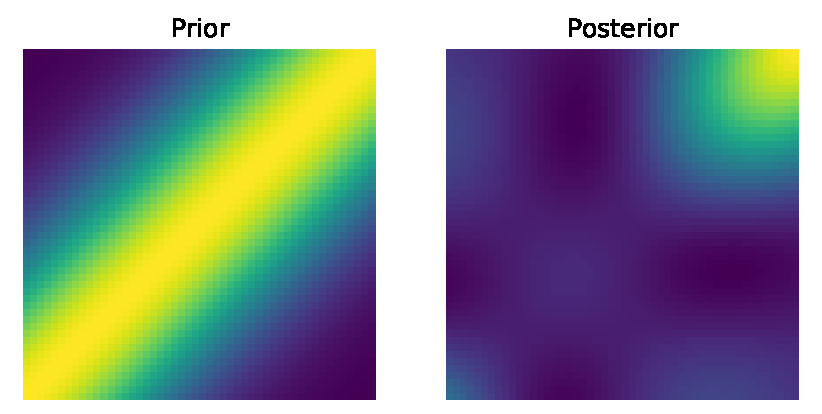
\includegraphics[width=0.6\textwidth]{pics/CovPosterior}
\caption{The covariance matrix before and after conditioning. The lighter areas show higher (co)variance. The part of the domain on the right, where no observations were made, is visible as entries with high variance in the top right.}
\label{fig:CovPOst}

\end{center}
\end{figure}

As introduced in Section \ref{sec:Marg}, the marginal likelihood can also be computed. It is used in the procedure for optimizing the hyperparameters of the chosen kernel function. Marginalizing over 















\section{The Statistical Finite Element Method}
The FEM is based on a model in form of a differential equation which is used to describe some kind of phenomenon, in the case of this thesis vibroacoustics, as accurately as possible. However, every model is only an approximation of reality which gives rise to a model inadequacy error: There is some unknown physics hidden between the model and reality. By collecting data, basically measuring reality with some kind of measurement error, that discrepancy $d$ between model and reality can be infered. That is what statFEM aims to do: It finds a new model, based on data, which solves the model inadequacy of the FEM.

\paragraph{The Statistical Generating Model}
Measuring data always involves a measurement error: One can never measure any physical quantity without some measurement noise. Therefore, the so-called statistical generating model \cite{girolami2021}, \cite{kennedy2001} for a vector of $n_y$ measurements $\bm{y} \in \mathbb{R}^{n_y}$, 
%
\begin{equation}
\bm{y} = \bm{z} + \bm{e} = \rho \bm{P} \bm{u} + \bm{d} + \bm{e} \; ,
\label{eqn:statGen}
\end{equation}
%
consists of response of the true underlying process $\bm{z} \in \mathbb{R}^{n_y}$ at the measurement points and the measurement noise $\bm{e} \in \mathbb{R}^{n_y}$. The true process $\bm{z}$ can further be expressed as a combination of the used model $\bm{u} \in \mathbb{R}^{n_u}$, which tries to describe the true process, and a model discrepancy error $d$ which accounts for the model not being a completely accurate representation of the true physics. The model is scaled using the scaling parameter $\rho \in \mathbb{R}$. It can be evaluated at $n_u$ points which are determined by the FEM mesh but only its evaluations at the measurement points are taken into account by using the projection matrix $\bm{P} \in \mathbb{R}^{n_y \times n_u}$. $n_u$ is the number of the so-called degrees of freedom of the domain, i.e. the number of nodes on which a solution is approximated.
%
$e$ is modeled as a multivariate Gaussian 
%
\begin{equation}
\bm{e} \sim p(\bm{e}) = \mathcal{N}(\bm{0}, \bm{C_e})
\end{equation}
with zero mean and the covariance matrix $\bm{C_e} = \sigma_e^2 \bm{I}$ which adds the measurement noise to each entry of $\bm{z}$.
%
The model discrepancy error is, in order to account for a possibly complex behavior, modeled as a GP
\begin{equation}
\bm{d} \sim p(\bm{d} | \sigma_d, l_d) = \mathcal{N}(\bm{0},\bm{C_d})
\end{equation}
which $\sigma_d, l_d$ the unknown parameters of a squared exponential kernel function. Evaluating it at the measurement positions, the GP is represented by a multivariate Gaussian with a covariance matrix $\bm{C_d} \in \mathbb{R}^{n_y \times n_y}$.




\paragraph{Basic statFEM procedure}
statFEM can basically be broken down into three major steps \cite{girolami2021}. The first one is applying Bayesian inversion to the FEM part of the solution. The prior GP is constructed and evaluated before data is introduced. Equations are derived which incorporate the data in order to compute a posterior density for the FEM solution GP. The equations for that solution are dependent on certain hyperparameters. These are estimated in the second step: For each of the hyperparameters a posterior density is calculated using a prior and the marginal likelihood. The third and last step is in principle finding a proper mesh size which is able to describe data the best. This last step may appear rather unimportant since usually in FEM the consensus is that a finer mesh leads to a more accurate result. However, it will be demonstrated that the optimum element size strongly depends on the value of certain hyperparameters estimated in step 2 and that there is a correlation between relatively inaccurate statFEM results and a too small element size.

\subsection{Posterior of the FEM Forward Model}

\paragraph{Assembling the FEM System Matrix}
The FEM assembly and solving is handled by Fenics. To compute the system matrix and to later solve for the vector of unknowns, the PDE has to be defined in a variational formulation as a boundary value problem.
At first, the FEM solver is initiated by defining the domain, the wished number of elements and the kind of elements to be used. In this example, a 1 dimensional mesh with Lagrange basis functions is used.
\begin{python}
def __init__(self, nMC = 200):
	self.dom_a = 0.0 #domain boundaries
	self.dom_b = 1.0
	self.ne	= 100 #number of elements
	self.mesh = IntervalMesh(self.ne,self.dom_a,self.dom_b) #define mesh
	self.bbt = self.mesh.bounding_box_tree()
	self.coordinates = self.mesh.coordinates() # vertices vector
	self.V = FunctionSpace(self.mesh, "Lagrange", 1) # Function space
\end{python}
The variational formulation for the chosen PDE consists of a linear form $L$ and a bilinear form $a$. These need to be specified individually for Fenics. The boundary condition is set to $u_0 = 0.0$ for both boundaries in the 1D mesh. The system matrix $A$ can be returned by calling \mintinline{python}{A = assemble(a)}. The boundary conditions are applied to $A$ after assambly.

\begin{minted}
[
frame=lines,
framesep=2mm,
baselinestretch=1.2,
bgcolor=backcolour,
fontsize=\footnotesize,
linenos
]
{python}
def doFEM(self):
	# Define Dirichlet boundary (x = 0 or x = 1)
	def boundary(x):
		return x[0] < (self.dom_a + DOLFIN_EPS) or x[0] > self.dom_b - DOLFIN_EPS
	# Define boundary condition
	u0 = Constant(0.0)
	self.bc = DirichletBC(self.V, u0, boundary)
	# Define variational problem
	self.u = TrialFunction(self.V)
	self.v = TestFunction(self.V)
	# find index of cell which contains point.
	class DoGP(UserExpression):
		def eval(self, value, x):
			collisions1st = bbt.compute_first_entity_collision(Point(x[0])) 
			value[0] = f_vals[collisions1st] # f is constant in a cell.
		def value_shape(self):
			return ()
	f_vals = self.draw_FEM_samples(coordinates)
	f_vals = f_vals[0]
	f = DoGP()
	
	a = dot(grad(self.u), grad(self.v))*dx #variational Problem
	L = f*self.v*dx

	A = assemble(a)
	b = assemble(L)
	self.bc.apply(A, b)
	
	U = self.u.vector()
	solve(A, U, b)
	return U, A

\end{minted}


\paragraph{Generate and Sample From Source Term GP}
The differential equation is treated from a Bayesian viewpoint: all parameters are random variables. For dependent parameters, such as a source term $f(x)$ dependent on the spatial coordinate, not a single distribution but a Gaussian Process is applied. Therefore prior to solving the FEM linear system, the parameter $ \mathcal{GP} ( \bar{f},C_f)$ is sampled. That sample is evaluated for each cell in the FEM mesh which makes it necessary to assemble the system matrix with that in mind. 
$\bar{f}$ is set to a prescribed value. $C_f$ is calculated using the prescribed hyperparameters of the chosen kernel function. As an example, a sample from $ \mathcal{GP} ( \bar{f},C_f)$ can be drawn for a Matern kernel by calling
\begin{minted}
[
frame=lines,
framesep=2mm,
baselinestretch=1.2,
bgcolor=backcolour,
fontsize=\footnotesize,
linenos
]
{python}
def sample_f(self):
	c_f = self.matern_log(self.coordinates,
		self.coordinates, l=np.log(lf), sig=np.log(sigf))
	f_mean = (np.pi)**2*(1/5)*np.ones(self.ne+1)
	fGP = np.random.multivariate_normal(
		mean = f_mean, cov=c_f,
		size=10)
\end{minted}
Here, the Matern kernel accepts only the $\log$ of the parameters $lf$ and $sigf$.

\paragraph{Generate and sample from the diffusion coefficient GP}
If the diffusion coefficient $\kappa$ is assumed to be a random variable and dependent on $x$, it can be modeled as a GP as well and there holds
\begin{equation}
\kappa \sim \mathcal{GP}(\bar{\kappa},C_{\kappa})
\end{equation}

\paragraph{Computing the FEM Prior}
Having the GPs for the input parameters defined, the FEM system of equations can be solved. With the input parameters defined as a GP, also the FEM solution is going to be a GP. Therefore, 
\begin{equation}
u \sim \mathcal{GP}(\bar{u}, C_u)
\end{equation}
is to be calculated. Multiplying the FEM system matrix by $\bm{A}^{-1}$ from the left there holds
\begin{equation}
\bm{u} = \bm{A}^{-1}\bm{f} \;.
\end{equation}
\cite[p. 1428]{arens2015} states that the expectation operator $\mathbb{E}$ is linear for independent random variables $X_1,X_2,...,X_n$ what means that
\begin{equation}
\mathbb{E}\left[  \sum_{i=1}^n X_i \right] = \sum_{i=1}^n \mathbb{E}[X_i] \;.
\end{equation}
A GP can be described by a set of independent normally distributed random variables. Because of the linearity there holds
\begin{equation}
\bar{u} = \mathbb{E}[\bm{A}^{-1} \bm{f}] = \bm{A}^{-1} \mathbb{E}[\bm{f}] = \bm{A}^{-1} \bar{f}
\end{equation}
and, acc. to \cite{schon2011, bardsley2018}, making use of the definition of covariance (\ref{eqn:Covariance}),
\begin{align}
\begin{split}
C_u &= \mathbb{E}[(\bm{u}-\bar{u})(\bm{u}-\bar{u})^T] \\
	&= \mathbb{E}\left[\left((\bm{A}^{-1} \bm{f}) - (\bm{A}^{-1} \bar{f}) \right) \left( (\bm{A}^{-1} \bm{f}) - (\bm{A}^{-1} \bar{f}) \right)^T   \right]\\
	&= \mathbb{E}\left[  \left( \bm{A}^{-1}(\bm{f}-\bar{f})   \right)  \left( \bm{A}^{-1}(\bm{f}-\bar{f})   \right)^T  \right]\\
	&= \mathbb{E} \left[    \bm{A}^{-1} ( \bm{f} - \bar{f} ) ( \bm{f} - \bar{f} )^T \bm{A}^{-T}   \right]\\
	&= \bm{A}^{-1}   \mathbb{E}\left[ (\bm{f}-\bar{f}) (\bm{f}-\bar{f})^T   \right] \bm{A}^{-T} \\
	&= \bm{A}^{-1} C_f \bm{A}^{-T}  \;.
\end{split}
\end{align}
%	 \\
%	 \\
%	
There fore there holds for the multivariate Gaussian, which describes the new $\bm{u} \sim \mathcal{GP}(\bar{u}, C_u)$
\begin{equation}
\bm{u} \sim p(u) = \mathcal{N} \left( A^{-1} \bar{f}, A^{-1} C_f A^{-T}  \right) \;.
\label{eqn:u_GP_disc}
\end{equation}
As visible in (\ref{eqn:u_GP_disc}), there holds for $\bar{u}$
\begin{equation}
\bar{u} = A^{-1} \bar{f} \; ,
\end{equation}
which can be computed using Python by calling
\begin{python}
def get_U_mean(self):
	u_mean = Function(self.V)
	U_mean = u_mean.vector()
	b_mean = assemble(f_mean*self.v*dx) 
	self.bc.apply(b_mean)
	solstd,A = self.doFEM()  # solstd is unused here.
	solve(A,U_mean,b_mean)
	return U_mean .
\end{python}
\label{lst:get_u_mean}
$C_u$ is obtained by calculating
\begin{equation}
A^{-1} C_f A^{-T} \; .
\end{equation}
In Python code there holds
\begin{python}
def get_C_u(self):
	C_f = self.get_C_f()
	solstd,A = self.doFEM()
	ident = np.identity(len(self.coordinates))
	self.bc.apply(A)
	A = A.array()
	A_inv = np.linalg.solve(A,ident)
	thresh = 1e-16
	C_u = np.dot( np.dot(A_inv,C_f), np.transpose(A_inv))
	C_u = C_u + 1e-16*(self.sigf**2)*ident
	c_u = np.transpose(self.integratedTestF) * C_u * self.integratedTestF
	return C_u .
\end{python}
\label{lst:get_C_u}
With $\bar{u}$ and $C_u$ the GP for the prior is completely defined. 
\paragraph{Find Prior Mean and Variance}
Once the prior is computed, it can be sampled. The mean is already given but the parameters of the underlying GP are unknown. It is possible to evaluate $C_u$ for the standard deviation with
\begin{equation}
\bm{\sigma_u} =  \mathrm{diag}(C_u).
\label{eqn:varCu}
\end{equation}
This yields the diagonal entries of the covariance matrix in a vector which now represents the variance at all test points. 
In Python
\begin{minted}
[
frame=lines,
framesep=2mm,
baselinestretch=1.2,
bgcolor=backcolour,
fontsize=\footnotesize,
linenos
]
{python}
C_u_sig = np.sqrt(np.diagonal(C_u))
\end{minted}
solves (\ref{eqn:varCu}).

\paragraph{The Projection Matrix $P$}
The projection matrix $P \in \mathbb{R}^{n_y \times n_u}$ is constructed by evaluating all $n_u$ FEM ansatz functions of the mesh at the $n_y$ measurement positions $y_i$. For each node there is a corresponding ansatz function which can be evaluated all over the domain. The result is a sparse matrix with most entries zero and only those entries non-zero which correspond to the ansatz functions $\Phi_i(\bm{\bm{x}})$ associated with the finite element in which the measurement positions lie. The matrix is used below to project the matrices resulting from the FEM prior onto the coordinates of the observations. Figure \ref{fig:PIllust} shows how the individual entries of $P$ are created for a 1D problem. Observation points, i.e. the training points, are displayed in red whereas all other points, i.e. test points, are displayed in green. The hat functions are $1$ only at one single node.
%
\begin{figure}[!ht]
\begin{center}

\begin{tikzpicture}[remember picture,scale=\textwidth/25.0cm,samples=200]
	\begin{pgfonlayer}{nodelayer}
		\node [style=none] (1) at (7, 0) {};
		\node [style=none] (2) at (-7, 0) {};
		\node [style=none] (3) at (-5, 0) {};
		\node [style=none] (4) at (-3, 0) {};
		\node [style=none] (5) at (-1, 0) {};
		\node [style=none] (6) at (1, 0) {};
		\node [style=none] (8) at (5, 0) {};
		\node [style=none] (9) at (3, 0) {};
		\node [style=none] (10) at (-7, 3) {};
		\node [style=none] (11) at (8, 0) {};
		\node [style=none] (12) at (7, 0) {};
		\node [style=none] (13) at (8, 0) {};
		\node [style=none] (14) at (8, 0) {};
		\node [style=green] (15) at (-7, 0) {};
		\node [style=green] (16) at (-5, 0) {};
		\node [style=green] (17) at (-3, 0) {};
		\node [style=green] (18) at (-1, 0) {};
		\node [style=green] (19) at (1, 0) {};
		\node [style=green] (20) at (3, 0) {};
		\node [style=green] (21) at (5, 0) {};
		\node [style=green] (22) at (7, 0) {};
		\node [style=none] (23) at (8.25, -0.25) {};
		\node [style=none] (24) at (8.25, 0) {$x$};
		\node [style=none] (32) at (-7.25, 2) {};
		\node [style=none] (33) at (-6.75, 2) {};
		\node [style=none] (34) at (-7.25, 2) {};
		\node [style=none] (35) at (-7.5, 2) {$1$};
		\node [style=none] (36) at (-7, 2) {};
		\node [style=none] (37) at (-5, 2) {};
		\node [style=none] (38) at (-3, 2) {};
		\node [style=none] (39) at (-1, 2) {};
		\node [style=none] (40) at (1, 2) {};
		\node [style=none] (41) at (3, 2) {};
		\node [style=none] (42) at (5, 2) {};
		\node [style=none] (43) at (7, 2) {};
		\node [style=none] (44) at (-7, -0.5) {$0$};
		\node [style=none] (45) at (-5, -0.5) {$1$};
		\node [style=none] (46) at (-3, -0.5) {$2$};
		\node [style=none] (47) at (-1, -0.5) {$3$};
		\node [style=none] (48) at (1, -0.5) {$4$};
		\node [style=none] (49) at (3, -0.5) {$5$};
		\node [style=none] (50) at (5, -0.5) {$6$};
		\node [style=none] (51) at (7, -0.5) {$7$};
		\node [style=none] (52) at (-5, 2.5) {$\varphi_1$};
		\node [style=none] (53) at (-3, 2.5) {$\varphi_2$};
		\node [style=none] (54) at (-1, 2.5) {$\varphi_3$};
		\node [style=none] (55) at (1, 2.5) {$\varphi_4$};
		\node [style=none] (56) at (3, 2.5) {$\varphi_5$};
		\node [style=none] (57) at (5, 2.5) {$\varphi_6$};
		\node [style=none] (58) at (7, 2.5) {$\varphi_7$};
		\node [style=none] (59) at (-6.5, 2.5) {$\varphi_0$};
		\node [style=new style 0] (60) at (-5, 0) {};
		\node [style=new style 0] (61) at (1, 0) {};
		\node [style=new style 0] (62) at (3, 0) {};
		\node [style=none] (63) at (-5, -1.25) {$y_0$};
		\node [style=none] (64) at (1, -1.25) {$y_1$};
		\node [style=none] (65) at (3, -1.25) {$y_2$};
	\end{pgfonlayer}
	\begin{pgfonlayer}{edgelayer}
		\draw [in=180, out=0] (2.center) to (1.center);
		\draw [style=arrow] (14.center) to (12.center);
		\draw [style=arrow, in=90, out=-90] (10.center) to (2.center);
		\draw [style=line] (15) to (22);
		\draw [style=line] (32.center) to (33.center);
		\draw [style=blue line] (36.center) to (16);
		\draw [style=red line] (15) to (37.center);
		\draw [style=red line] (37.center) to (17);
		\draw [style=red line] (17) to (18);
		\draw [style=red line] (18) to (19);
		\draw [style=red line] (19) to (20);
		\draw [style=red line] (20) to (21);
		\draw [style=red line] (21) to (22);
		\draw [style=green line] (16) to (38.center);
		\draw [style=green line] (38.center) to (18);
		\draw [style=green line] (18) to (19);
		\draw [style=blue line] (16) to (17);
		\draw [style=blue line] (17) to (39.center);
		\draw [style=blue line] (39.center) to (19);
		\draw [style=red line] (18) to (40.center);
		\draw [style=red line] (40.center) to (20);
		\draw [style=green line] (19) to (41.center);
		\draw [style=green line] (41.center) to (21);
		\draw [style=blue line] (20) to (42.center);
		\draw [style=blue line] (42.center) to (22);
		\draw [style=red line] (21) to (43.center);
	\end{pgfonlayer}
\end{tikzpicture}

\begin{equation}
P =
\begin{bmatrix}
0 & \rn{101}{1} & 0 & 0 & 0 & 0 & 0 & 0\\
0 & 0 & 0 & 0 & \rn{102}{1} & 0 & 0 & 0\\
0 & 0 & 0 & 0 & 0 & \rn{103}{1} & 0 & 0
\end{bmatrix}
\end{equation}

\caption{The matrix $P$ contains the values of the FEM ansatz functions belonging to the nodes on which observations are available. Since linear Lagrange elements yield $1$ at their respective node number and $0$ on all other nodes, $P$ consists of only $1$s and $0$s.}
\label{fig:PIllust}


\begin{tikzpicture}[overlay,remember picture]
	\draw [->] (3) to [out=-40,in=30] (101);
	\draw [->] (6) to [out=-50,in=60] (102);
	\draw [->] (9) to [out=-120,in=60](103);
\end{tikzpicture}
\end{center}
\end{figure}
%
This computation for linear ansatz functions can easily be implemented in Python using Fenics:
\begin{python}
def getP(self,y_points):
	ny = len(y_points)
	P = np.zeros((ny, self.ne+1), dtype = float) #with ne the number of elements
	for j,point in enumerate(y_points):
		x = np.array([point])
		x_point = Point(x)
		bbt = self.mesh.bounding_box_tree()
		cell_id = bbt.compute_first_entity_collision(x_point)
		cell = Cell(self.mesh, cell_id)
		coordinate_dofs = cell.get_vertex_coordinates()
		values = np.ones(1, dtype=float)
		for i in range(self.el.space_dimension()): 
			phi_x = self.el.evaluate_basis(np.array(i),x 
				,np.array(coordinate_dofs),cell.orientation())
			P[j,cell_id+i] = phi_x
	self.Pu = np.dot(P,self.U_mean)
	return P
\end{python}
\label{lst:getP}
\paragraph{Calculate $C_e$}
$C_e$ is the measurement error term. It is defined in Python by
\begin{minted}
[
frame=lines,
framesep=2mm,
baselinestretch=1.2,
bgcolor=backcolour,
fontsize=\footnotesize,
linenos
]
{python}
def get_C_e(self,size):
	sige_square = 2.5e-5
	C_e = sige_square * np.identity(size)
	return C_e
\end{minted}

\paragraph{Calculate $C_d$}
The model discrepancy term $C_d$ is modeled as a GP with mean $\bar{d} = 0$. Therefore it can be obtained by calling
\begin{minted}
[
frame=lines,
framesep=2mm,
baselinestretch=1.2,
bgcolor=backcolour,
fontsize=\footnotesize,
linenos
]
{python}
def get_C_d(self,y_points,ld, sigd):
	C_d = self.matern_log(y_points, y_points, l=ld, sig=sigd)
	return C_d
\end{minted}
The points in the domain and the hyperparameters have to be provided in order to calculate the covariance function. The latter ones are not yet known and need to be estimated, see below for a thorough explanation on that.

\subsection{Inference of the Posterior Density}
To infer the posterior density, observed data is necessary. These can be obtained by either actually measuring a physical process or by generating synthetic data which allows developing and improving the statFEM model already before having to set up an experiment and take real measurements beforehand.
%
Sampling from a synthetic source or from the real physical response yields the observation vector
%
\begin{equation}
\bm{y} = \bm{z} + \bm{e}
\end{equation}
%
with $\bm{z}$ the real response and $\bm{e}$ the measurement error which is also a part of $\bm{y}$ for the synthetic observations. It can be seen that the model mismatch error $\bm{d}$ is, as opposed to (\ref{eqn:statGen}), not part of the equation because it is only part of the FEM modeling error. 
%
The data is observed on multiple measurement points $y_i$ throughout the domain. It can be chosen if the data is assumed to be deterministic or to be random. For the deterministic case only one value is measured for each measurement point. In the random case many measurements are taken per point what leads to a probability distribution for each point.
%
Now, Bayes' rule can be applied to update the prior with the observations \cite{girolami2021}: 

\begin{equation}
p(\bm{u}|\bm{y}) = \frac{p(\bm{y}|\bm{u})p(\bm{u})}{p(\bm{y})} \propto p(\bm{y}|\bm{u})p(\bm{u}) \;.
\label{eqn:bayesPrior}
\end{equation}
The marginal likelihood is, in form of a normalization term, going to be reintroduced in the end. Both densities $p(\bm{y}|\bm{u})$ and $p(\bm{u})$ are considered multivariate Gaussian, see (\ref{eqn:statGen}) and (\ref{eqn:MultivariateGaussian}):
\begin{align}
p(\bm{y}|\bm{u}) &\sim \mathcal{N} (\rho P \bm{u}, C_d + C_e) \\
p(\bm{u}) &\sim \mathcal{N}(\bm{\bar{u}},C_u)
\end{align}
%
That property makes the multiplication simple, again excluding the marginal likelihood:
\begin{equation}
p(\bm{u}|\bm{y}) \propto  \exp(  (\rho P \bm{u} -\bm{y})^T (C_d + C_e)^{-1} (\rho P \bm{u} -\bm{y})  ) \exp(  (\bar{\bm{u}} - \bm{u})^T C_u^{-1}  )
\end{equation}
Following \cite{girolami2021}, with
\begin{align}
\begin{split}
B &= \rho^2 P^T (C_d +C_e)^{-1} P + C_u^{-1} \\
\bm{a} &= \rho P^T (C_d +C_e)^{-1} \bm{y} + C_u^{-1} \bm{\bar{u}}
\end{split}
\end{align}
there holds
\begin{align}
\begin{split}
p(\bm{u}|\bm{y}) &\propto \exp(\bm{u}^T B \bm{u} - 2\bm{a}^T\bm{u} + ... ) \\
&= \exp( (B^{-1} \bm{a} - \bm{u} )^T  B (B^{-1} \bm{a} - \bm{u} ) ) \;.
\label{eqn:p_u_y_unnorm}
\end{split}
\end{align}
Comparing \ref{eqn:p_u_y_unnorm} to \ref{eqn:MultivariateGaussian} it can be argued that \ref{eqn:p_u_y_unnorm} can be normalized to 
\begin{equation}
p(\bm{u}|\bm{y}) = \frac{1}{\sqrt{(2\pi)^{n_u} \lvert B \rvert}} \exp( (B^{-1} \bm{a} - \bm{u} )^T  B (B^{-1} \bm{a} - \bm{u} ) )
\end{equation} 
%
The result of this operation is
%
\begin{equation}
p(u|y) = \mathcal{N}(\bar{u}_{|y}, C_{u|y})
\label{eqn:statFEMConditioned}
\end{equation}
%
with
%
\begin{equation}
\bm{\bar{u}}_{|y} = C_{\bm{u}|\bm{y}} \left(   \rho P^T  (C_d + C_e)^{-1}  y  +  C_u^{-1}  \bar{u}   \right)
\end{equation}
and
\begin{equation}
C_{\bm{u}|\bm{y}} = \left(      \rho^2  P^T   (C_d + C_e)^{-1}  P  +  C_u^{-1}    \right)^{-1} \;.
\end{equation}
To avoid having to invert matrices with the size of $n_u \times n_u$, the Sherman-Morrison-Woodbury identity \cite{riedel1992} is applied \cite{girolami2021} in order to only invert matrices with the size of $n_y \times n_y$ which yields
\begin{equation}
C_{\bm{u}|\bm{y}} = C_u - C_u P^T (\frac{1}{\rho^2} (C_d + C_e) + P C_u P^T)^{-1} P\,C_u \;.
\end{equation}

The same result can be achieved using the approach discussed in \ref{sec:GPcond}. The joint probability for the FEM prior and the observed data states
\begin{equation}
p(\bm{u},\bm{y}) = \begin{bmatrix}
           \bm{u}\\
          \bm{y}
         \end{bmatrix} \sim \mathcal{N}\left( \begin{bmatrix}
           \bar{\bm{u}}  \\
           \bar{\bm{y}}
         \end{bmatrix}, \begin{bmatrix}
C_u & \rho C_u P^T \\
\rho P C_u  & \rho^2 P C_u P^T + C_d + C_e 
\end{bmatrix}  \right)
\end{equation}
which can now be conditioned according to \ref{eqn:ConditioningDistr}, which ultimately leads to \ref{eqn:statFEMConditioned}.



\subsection{Probabilistic FEM Prior}
The prior before observation is obtained by computing the FEM response $u_h$ of the PDE given all parameters. The random parameters are modeled as GPs. Thereby result a mean $\bar{u}_h$ and a covariance matrix $C_u$. For this being the prior, the hyperparameters for the source term GP are chosen deterministically. The covariance matrix is obtained by calculating $C_u = A^{-1} C_{par} A^{-T}$ with $A$ the FEM system matrix and $C_{par}$ the covariance matrix of the respective random parameter's GP. The mean can easily be determined by calculating the deterministic mean of the FEM by using only the GP's mean.
The resulting response $u_h$ is, since it is discretized and not continuous, a multivariate Gaussian distribution.
%
To check convergence of the FEM model, it can be compared to the exact analytically determined system response $u$. 
%
It is assumed that there is a difference between the exact and the calculated FEM response to the true system response. That difference will be reduced by updating the prior with observations.
%
With the basic FEM code set up for a random source term and a deterministic diffusion coefficient, $\bar{u}$ can be obtained by calling


$C_u$ can be obtained by calling

For numerical reasons a small nugget is added to the diagonal of $C_u$. This does not significantly change the result but allows using the Cholesky decomposition.
With $\bar{u}$ and $C_u$ at hand the prior GP is defined as $u \sim \mathcal{GP}(\bar{u},C_u)$. To check if the covariance matrix is correct, a MC approximation $\bar{u}_{MC}$ of the mean can be computed by evaluating the GP $n_{MC}$ times and taking the average. As visible in Figure \ref{fig:u_mean_conv}, the error of $\bar{u}_{MC}$ converges to zero with a slope of 2 on a logarithmic scale. Therefore, $C_u$ indeed has a mean of $\bar{u}$.
The MC samples can be drawn via
\begin{python}
def samplePrior(self):
	U_mean = self.get_U_mean()
	C_u = self.get_C_u()
	priorGP = np.random.multivariate_normal(
		mean = U_mean, cov=C_u,
		size=self.nMC)
	return priorGP
\end{python}

Code for calculating u
direct calculation
MC approximation from GP samples
-error bands

Code for calulating Cu
direct calucaltion
MC approximation
error bands


\begin{figure}[!ht]
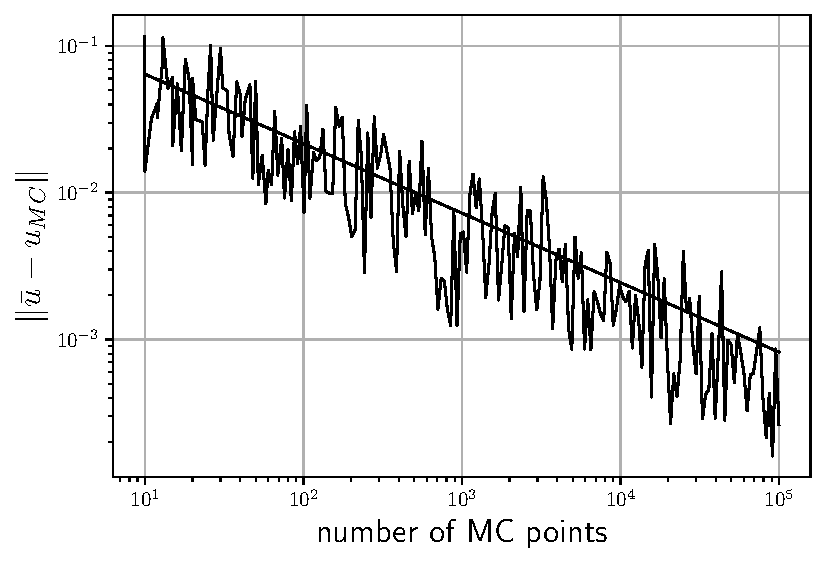
\includegraphics[width=0.6\textwidth]{pics/MCerrorConv.pdf}
\centering
\caption{Convergence of the error norm for the FEM prior mean with a slope of 2 on a log-log scale.}
\label{fig:u_mean_conv}
\end{figure}




\subsection{Estimation of Hyperparameters }

Below it was already stated that the hyperparameters for computing the model discrepancy covariance matrix $\bm{C_d}$ are not known. The scaling factor $\rho$ is not known, as well. The measurement data can be used to estimate these parameters, collected in the hyperparameter vector $\bm{w}$. This is done using Bayes' rule again: There holds
%
\begin{equation}
p(\bm{w}|\bm{y}) = \frac{P(\bm{y}|\bm{w}) p(\bm{w})}{\int P(\bm{y}|\bm{w}) p(\bm{w}) \, \mathrm{d}\bm{w}}
\label{eqn:bayesHyperp}
\end{equation}
%
for the posterior. The posterior $p(\bm{w}|\bm{y})$ states that the vector of hyperparameters $\bm{w}$ depends on the measurements data $\bm{y}$, which makes sense because the data is meant to be used to estimate and optimal $\bm{w}$. $p(\bm{w})$ is the prior for the hyperparameters. Obviously, maximizing the likelihood $P(\bm{y}|\bm{w})$ maximizes the posterior which basically means finding the set of hyperparameters which are most probable to explain $\bm{y}$. Comparing the likelihood $P(\bm{y}|\bm{w})$ with Bayes' rule as it was applied for the FEM solution prior in \ref{eqn:bayesPrior} shows that it has already been introduced before, namely as the marginal likelihood $p(\bm{y})$ in that case. It makes sense stating that $p(\bm{y}) = p(\bm{y}|\bm{w})$ because, following the statistical generating model \ref{eqn:statGen}, $\bm{y}$ is defined using the hyperparameters and therefore its probability function is conditional on $\bm{w}$. \cite[p.12]{girolami2021}
The denominator in \ref{eqn:bayesHyperp}, which only serves as a normalization constant, can be dropped if only a point estimate of the hyperparameters is needed. This approach is then indeed non-bayesian because no probability density of the hyperparameters is computed.
For multiple measurements $y_i$ with a total number of $n_o$ there holds, because it is assumed that individual measurements are independent \cite[p.9]{rasmussen2006},
\begin{equation}
P(\bm{Y}|\bm{w}) = \prod_{i=1}^{n_o} p(\bm{y_i}|\bm{w}) \; 
\end{equation}
which replaces $P(\bm{y}|\bm{w})$.
If no prior knowledge of the parameters is available, it is possible and even common to use an uninformative prior $p(\bm{w}) = 1$. \cite[p.433]{kennedy2001}
The equation then basically states that $p(\bm{w}|Y) \propto P(Y|\bm{w})$ which means that maximizing  $P(\bm{Y}|\bm{w})$, i.e. the likelihood to measure $Y$ given a set of hyperparameters, yields the optimal vector of hyperparameters for the given data. 
The marginal likelihood $P(\bm{y}|\bm{w})$, marginal because it has been marginalized over the function values $\bm{u}$ as in \ref{sec:Marg}, can be expressed as a Gaussian normal distribution
\begin{equation}
p(\bm{y}|\bm{w}) = \mathcal{N}(\rho \bm{P}\bar{u}, \bm{C_d}+\bm{C_e} + \rho^2 \bm{P} \bm{C_u} \bm{P}^T)
\end{equation}
because, as stated above, all components of the statistical generating model are Gaussian.
The equation for the corresponding PDF reads, in agreement with Section \ref{sec:MultiGauss},
\begin{equation}
p(\bm{y}|\bm{w}) = \frac{1}{(2 \pi)^{n/2} |\bm{K}|^{1/2} } \exp \left(   -\frac{1}{2} (\bm{y} - \rho \bm{P}\bar{u})^T \bm{K}^{-1} (y - \rho \bm{P}\bar{u})   \right)
\end{equation}
with
\begin{equation}
\bm{K} = \bm{C_d}+\bm{C_e} + \rho^2 \bm{P} \bm{C_u} \bm{P}^T \; .
\end{equation}
%
To make further calculations easier the exponential function can be removed by taking the negative $\log$ of the function \cite[p.113]{rasmussen2006}:
\begin{equation}
- \log p(\bm{y}|\bm{w}) = \frac{n}{2} \log(2 \pi) + \frac{1}{2} \log |\bm{K}| + \frac{1}{2}(\rho \bm{P}\bar{u} - \bm{y})^T \bm{K}^{-1} (\rho \bm{P}\bar{u} - \bm{y}) 
\label{eqn:neglog}
\end{equation}
This also improves numerical stability because products of possibly very small factors can become smaller than machine accuracy. The log replaces products with sums.
Because of taking the negative $\log$, (\ref{eqn:neglog}) now needs to be minimized instead of maximized. 
The individual terms fulfill different roles: 

\paragraph{Non-identifiability}
priors need to be informative, p12 statFEM
\cite{Eberly2000} MCMC can lead to wrong sets of parameters or doesn't converge.
\cite{Bayarri} \cite{kennedy2001}

\paragraph{Cholesky Decompositon}
\label{sec:Cholesky}
This follows \cite[p.93-95]{chambers1998}.
For numerical stability reasons, $\bm{K}^{-1}$ should not be calculated directly. Instead, the linear system is solved. Additionally, if $\bm{K}$ is symmetric and positive-semidefinite, computing the lower triangular matrix using the Cholesky decomposition 
\begin{equation}
\bm{K} = \bm{L}\bm{L}^T
\end{equation}
makes the calculation quicker and yields the also needed determinant of $\bm{K}$ as a by-product. 
A generic linear system is defined as $A x = b$. It is solved for $x$, so the inverse of $A$ is needed. In this case for (\ref{eqn:neglog}) there holds $A=\bm{K}$ and $b = y$, since the inverse of $\bm{K}$ is meant to be found. Defining $x = \bm{K}^{-1}y$ there holds
\begin{equation}
\bm{K} \bm{K}^{-1}  y = y
\end{equation}
%
With $\bm{L}$ the lower triangular matrix of $\bm{K}$ obtained by 
\begin{lstlisting}[language=Python]
L = scipy.linalg.cho_factor(K)
\end{lstlisting}
the linear system can now be solved for $x = \bm{L}y$ with
\begin{lstlisting}[language=Python]
K_inv_y = scipy.linalg.cho_solve(L, y) .
\end{lstlisting}

The determinant of any triangular matrix is defined as the product of its diagonal entries \cite{tomaskovic-moore}. Therefore the lower triangular matrix $\bm{L}$ can be used to efficiently calculate the determinant of $\bm{K}$. There holds
\begin{equation}
\mathrm{det} (\bm{K}) = \mathrm{det} (\bm{L}) \mathrm{det} (\bm{L}^T) = \mathrm{det} (\bm{L} ^2)
\end{equation}
and therefore
\begin{equation}
\mathrm{det} (\bm{K}) = \left(    \prod_{i=1}^{n_y}  \bm{L}_{i,i}  \right)^2
\label{eqn:CholDet}
\end{equation}
%
Since in (\ref{eqn:neglog}) the $\log$ likelihood is used, (\ref{eqn:CholDet}) can be simplified to a sum:
%
\begin{align*}
\log{\mathrm{det} (K)} &= \log{\mathrm{det} (L^2)} \\
&= 2 \sum_{i=0}^{n_y} \log{L_{i,i}}
\end{align*}

\subsubsection{Minimization of the Negative log-Likelihood}
The best possible set of hyperparameters $\bm{w}$ for (\ref{eqn:neglog}) to be as small as possible has to be found, i.e. the negative log-likelihood has to be minimized in order to get a model which represents given data the best. That can be achieved by using a gradient based optimizer or by sampling the parameter space with, e.g., a MCMC approach. Both find a point estimate for the set of hyperparameters which lead to the minimal negative log-likelihood. Caution has to be taken for problems in which the negative log-likelihood yields multiple local minima. \cite{Svensson2015} These and another, more simple, approach to find the minimum are given:
\paragraph{Random Sampling in the Parameter Space}
This method is used in this thesis because of its simplicity in implementation. For real-world applications it is not recommended since it is the slowest of all three proposed methods.
\begin{figure}[!ht]
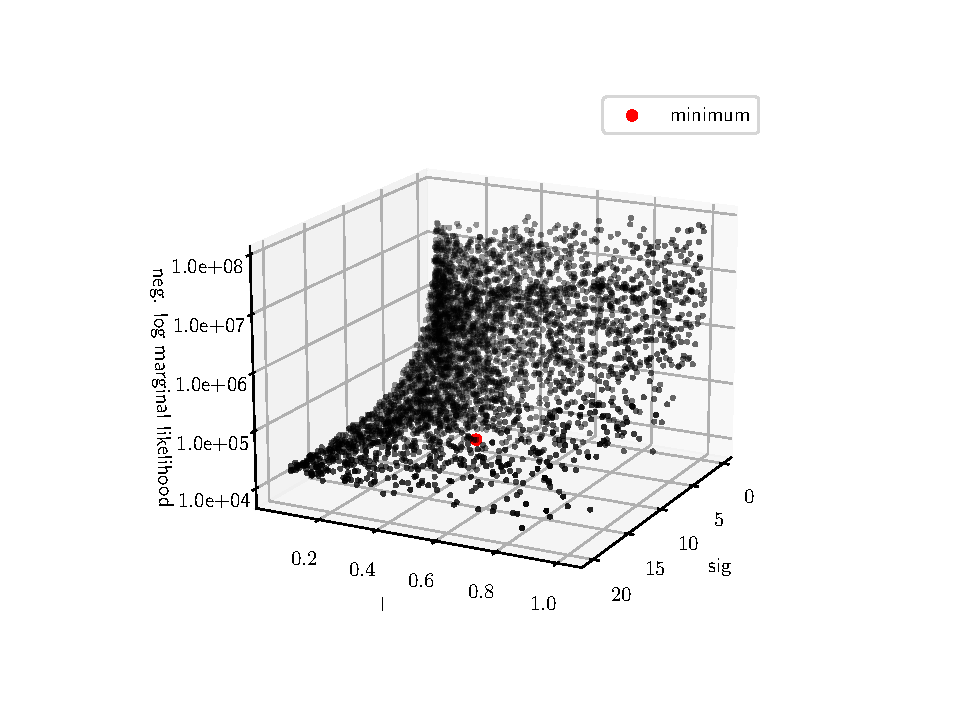
\includegraphics[width=1\textwidth]{pics/RandomHyperParSearch.pdf}
\centering
\caption{See the \href{https://github.com/herluc/herluc.github.io/blob/main/MLL.gif}{Animation} to get a better understanding of where the minimum lies. Sampling throughout a carefully predefined parameter space and solving for the negative log-likelihood yields a field of solutions. The set of hyperparameters is chosen which yields the smallest negative log-likelihood. The scaling factor $\rho$ is also part of the random sampling but not shown here. The found minimum is shown as a red dot.}
\label{fig:RandSampHyper}
\end{figure}
It works by sampling randomly in the hyperparameter space, solving \ref{eqn:neglog} and keeping the hyperparameter set which yields the lowest value. The better the hyperparameter-space is chosen, i.e. the better the prior describes the best combination of parameters already, the better the approximatin considering a fixed number of possible samples. For example, it makes sense to sample all parameters only for positive values,  the distance measure $l$ only for values smaller than the domain and the variance $\sigma$ only in the same order of magnitude as the FEM prior. Figure \ref{fig:RandSampHyper} gives an impression of how the samples are distributed.



\paragraph{MCMC}
Markov Chain Monte Carlo (MCMC) is a very efficient sampling method. Just as standard MC, it can be used to draw samples from a given distribution. The advantage of MCMC is now that an algorithm finds a relatively small set of samples which is able to describe the distribution very accurately. The result is a distribution for the hyperparameters of which e.g. the mean can be deduced. One common algorithm is the metropolis algorithm.
The metropolis algorithm is a special case of MCMC for a symmetric proposal distribution.
According to \cite[p.31]{girolami2021} the MCMC metropolis algorithm can be implemented with the following steps:
\begin{enumerate}
\item Sample a proposal density, e.g. a normal distribution, $q(w|v) = \mathcal{N}(v,\sigma^2_q I)$
\end{enumerate}




\paragraph{L-BGFS}
C. Zhu, R. H. Byrd, P. Lu, J. Nocedal, Algorithm 778: L-BFGS-B: Fortran subroutines for large-scale bound-constrained optimization, ACM
32Transactions on Mathematical Software (TOMS) 23 (1997) 550–560.

L-BGFS is a gradient based optimizer. It doesn't deliver a distribution for the hyperparameters but only a point estimate.
For the optimization with L-BGFS the derivative of (\ref{eqn:neglog}) is needed. It can be computed as follows.






\chapter{A statFEM Approach for Vibroacoustics}
In the previous chapters, the theoretical basis for an application of statFEM has been built. So now at first, in order to verify the methods and the programmed software, as a simple 1D problem the Poisson equation is going to be solved. Although having no direct connection to acoustics, it is a very common sample problem for numeric methods and thus there are many resources \cite{girolami2021} \cite{langtangen2019} with which the results can be compared.

Having verified the methods, the complexity can be increased to a 2D problem: The Helmholtz equation is solved. A suitable kernel function is chosen and the boundary conditions are applied. The problem is considered to part of the vibroacoustics field because one boundary condition resembles a vibrating plate under uncertainty and the acoustical behavior of the adjoining domain is studied.

\section{Simple 1D example}
\paragraph{Choice of PDE}
The Poisson equation 
%%
\begin{equation}
- \nabla \cdot \mu(x) \nabla u(x) = f(x)
\label{eqn:Poisson}
\end{equation}
%%
is chosen as the governing equation. It is an elliptic partial differential equation (PDE). In this work it is used as a simple 1D example to illustrate how the statistical FEM and especially the Gaussian Process Regression works.
The most standard form of it does not, contrary to this example, include $\mu(x) \in \mathbb{R}^+$ which is the diffusion coefficient dependent on the spatial variable $x$. The right-hand side consists of the source term $f(x)\in \mathbb{R}$. Both $\mu (x)$ and $f(x)$ are the free parameters in this case. The equation is solved for the unknown  $u(x)$ in the domain $\Omega = (0,1)$ with the boundary condition $u(x) = 0$ on $x=0$ and $x=1$.
%
For a first example there holds $\mu(x)=1$. $f(x)$ is modeled as a Gaussian Process: \cite{girolami2021}
%
\begin{equation}
f(\bm{x}) \sim \mathcal{GP} \left( \bar{f}(\bm{x}), c_f(\bm{x},\bm{x}')\right) \;.
\end{equation}
%
\paragraph{Construction of the GP}
The mean function of the GP is set to $\bar{f}(x) = 1.0$. For the covariance function at first a squared exponential kernel 
%
\begin{equation}
c_f(\bm{x},\bm{x}') =    \sigma_{f}^2 \exp \left(-  \frac{\left \| \bm{x}-{\bm{x}}' \right \|^2}{2l_{f}^2} \right )       
\label{eqn:sqEx_f}
\end{equation}
%
is used with the standard deviation $\sigma_{f} = 0.1$ and the length scale $l_{f} = 0.4$.
In Python the kernel is directly implemented as a function which takes two lists and the parameters as input variables \cite{murphy2012}

%
Here, the parameters are fixed but in a later example a method on how to infer the optimum position for these will be studied.

Having prepared the mean function and the kernel, which can be considered the prior in a GP regression setting, a sample of the GP can be drawn. For this points have to be chosen on which the kernel is evaluated. These are the test points and, according to [Cirak], correspond to the center of the FEM cells. This implies that there are as many test points as FEM cells and therefore the coordinates of the FEM mesh can directly be used to compute the covariance matrix. For that (\ref{eqn:sqEx_f}) is evaluated at $\bm{x} = \bm{x}'$ with $\bm{x}$ the vector of test points. 

A GP has the marginalization property: if you sample it at a finite number of points it yields a multivariate Gaussian distribution $\mathcal{N}(\bar{\bm{f}},\bm{C_f})$ with $\bar{\bm{f}}$ the mean vector and $\bm{C_f}$ the covariance matrix while still describing the underlying continuous sample.
According to \cite{rasmussen2006} sampling from a multivariate Gaussian distribution works as follows: To obtain $n$ samples from the prior, at first $n$ samples of a standard normal distribution, also called Gaussian white noise, $e \sim \mathcal{N}(0,1)$ have to be drawn. Computing the Cholesky decomposition of the covariance matrix $\bm{C_f} = LL^T$, which can also be thought of as taking the square root of a matrix, yields the lower triangular matrix $L$. Samples can now easily be drawn from $\bm{f} = \bar{\bm{f}} + Le$ which is a multivariate Gaussian distribution with a mean $\bm{f}$ and a covariance $\bm{C_f}$.

Sample: Normal distribution times std dev. GP with n points is basically a multivariate gaussian with n dimensions. therefore we need the std dev. for a univariate gaussian thats . 

For the observations made in a later step it is assumed that there is some measurement noise. This is modeled as an added variance $\sigma_{n}^2$ on the diagonal of the prior covariance matrix. An additional effect of this added noise is the improved numerical stability of the covariance matrix which is important for computing the Cholesky decomposition.

The observations have been taken on samples of a GP $z(x) \sim \mathcal{GP}(\bar{z}(x),A^{-1}c_z(x,x')A^{-T})$ which uses the harmonic function
\begin{equation}
\bar{z}(x) = 0.2\sin(\pi x) + 0.02\sin(\pi x)
\end{equation}
as a mean and a Matern kernel with the hyperparameters $l_z=0.5$ and $\sigma_z = 0.15$ as covariance function. Figure \ref{fig:zGP} shows that the mean and therefore also the variance band is not as smooth as the prior: Amodel discrepancy error is present.
\begin{figure}[!ht]
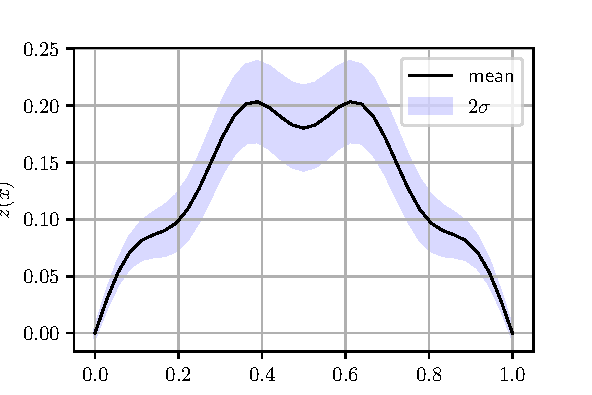
\includegraphics[width=0.6\textwidth]{pics/z_GP.pdf}
\centering
\caption{}
\label{fig:zGP}
\end{figure}
%


\subsection{FEM Prior}
The mean, $2\sigma$ confidence bands and realisations of the FEM prior are visible in Figure \ref{fig:FEMGP1D}. As expected, the general shape of the solutions follows the smooth behaviour of the Laplacian. The variance becomes larger the further away from the Dirichlet zero-boundary conditions.
\begin{figure}[!ht]
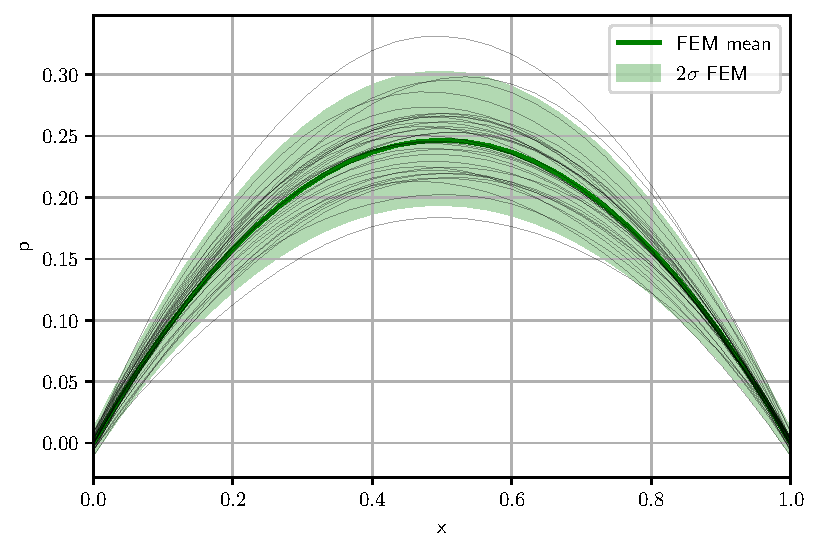
\includegraphics[width=0.65\textwidth]{pics/1DFEMprior.pdf}
\centering
\caption{FEM Prior for the 1D example. The mean and confidence band as well as samples drawn from the GP are shown. As the boundary conditions imply, both mean and variance are zero on the boundary of the domain.}
\label{fig:FEMGP1D}
\end{figure}






\subsection{Posterior}
For the posterior, at first one single sensor location was introduced at which one single measurement has been taken. The point has been picked arbitrarily and a measurement noise has been introduced. Already it is visible that the general shape of the FEM prior remains but itis scaled to the data. Also, the variance becomes smaller as there now is evidence on the true solution.
%
\begin{figure}[!ht]

\centering

	\begin{subfigure}[t]{.5\textwidth}
	\centering
	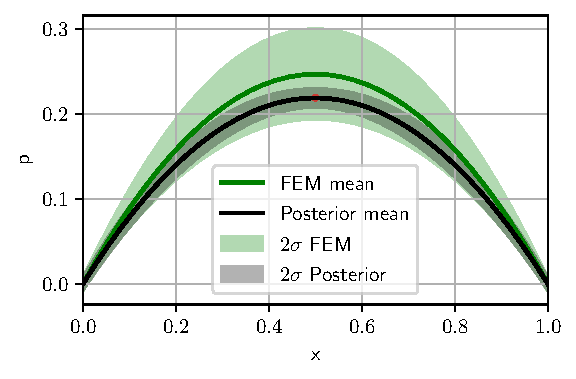
\includegraphics[width=1\linewidth]{../../Python/Results/1D/Model_Error/1o_1s/Result.pdf}
	\caption{One observation at one sensor location. Shape of FEM Prior remains but scaling and variance differ.}	
	\label{fig:OneSensor}
	\end{subfigure}%
	%\hfill
	\begin{subfigure}[t]{.5\textwidth}
	\centering
	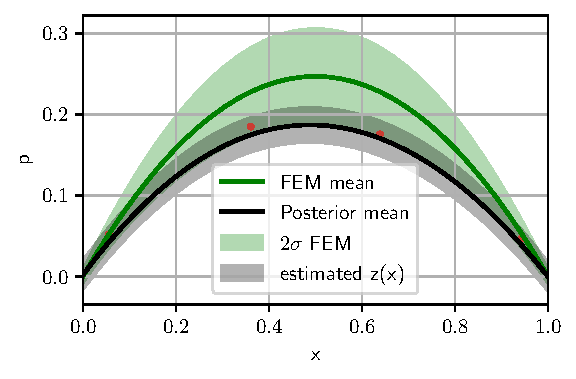
\includegraphics[width=1\linewidth]{../../Python/Results/1D/Model_Error/1o_4s/Result.pdf}
	\caption{Per observation point 1 individual observation was taken with a standard deviation of $2.5e-5$. }	
	\label{fig:4p10}
	\end{subfigure}
	
	\begin{subfigure}[t]{.5\textwidth}
	\centering
	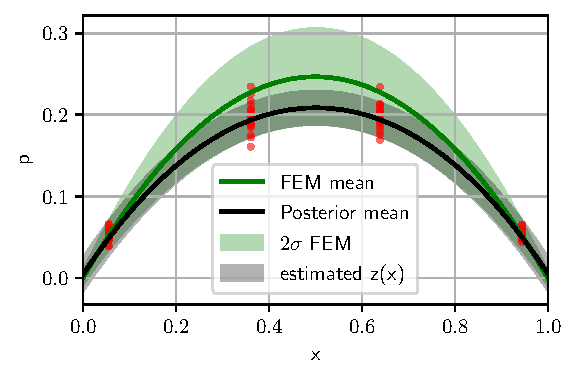
\includegraphics[width=1\linewidth]{../../Python/Results/1D/Model_Error/20o_4s/Result.pdf}
	\caption{Per observation point 20 individual observations were taken with a standard deviation of $2.5e-5$. }	
	\label{fig:DataCloseToCI2}
	\end{subfigure}%
	%\hfill
	\begin{subfigure}[t]{.5\textwidth}
	\centering
	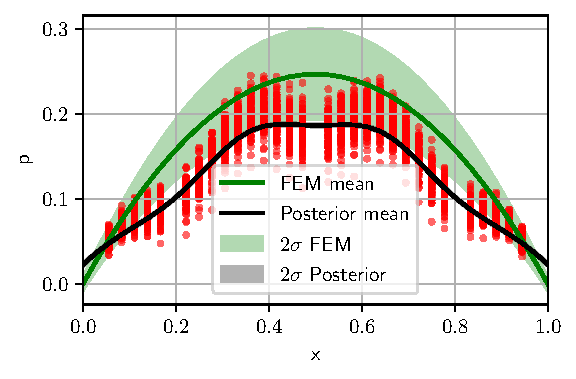
\includegraphics[width=1\linewidth]{../../Python/Results/1D/Model_Error/100o_30s/Result.pdf}
	\caption{Per observation point 100 individual observations were taken with a standard deviation of $2.5e-5$. }	
	\label{fig:DataCloseToCI2}
	\end{subfigure}

\caption{The posterior for different measurement scenarios. The more sensor locations are introduced and the more observations are taken, the smaller the variance gets.}	
	
\label{fig:OneSensor}
\end{figure}
%
Figure \ref{fig:4p10} shows that, if the observations are made slightly out of the FEM confidence band, a posterior can be inferred which fits to the data. In this example multiple measurement locations were chosen and one single observation has been taken per point. The variance drops significantly and the solution is scaled to fit the data.
%
As Figure \ref{fig:DataCloseToCI2} shows, increasing the number of obervations per sensor leads to a smaller variance.

If now the observations are taken from a sample which does not resemble the overall shape of the FEM prior as closely, model error is introduced. Figure \ref{fig:ModelError1D} shows significantly more variance in the posterior as Figure \ref{fig:NoModelError1D}.
\begin{figure}[!ht]

	\begin{subfigure}[t]{.5\textwidth}
	\centering
	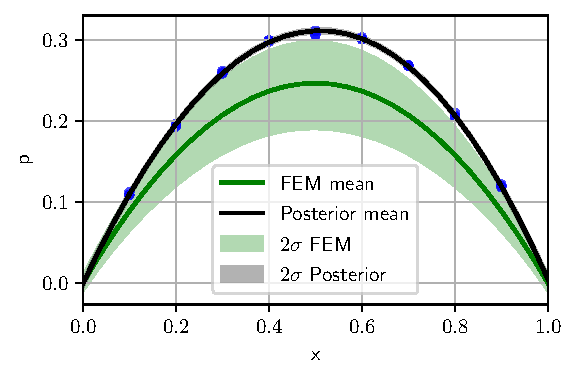
\includegraphics[width=1\linewidth]{../../Python/Results/1D/no_d_scaled_40proc.pdf}
	\caption{Observing data from a scaled sample of the FEM prior leads to a very small variance.}
		\label{fig:NoModelError1D}
	\end{subfigure}%
	\begin{subfigure}[t]{.5\textwidth}
	\centering
	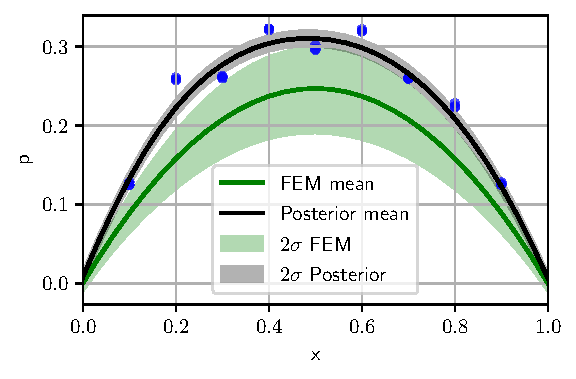
\includegraphics[width=1\linewidth]{../../Python/Results/1D/d_scaled40proc.pdf}
\centering
\caption{Introducing significant model error to the observations leads to a higher variance. It could be reduced by using more observations per sensor location.}
\label{fig:ModelError1D}
	\end{subfigure}

\caption{Comparison of the influence of different amounts of model error on the posterior variance.}
\label{fig:ModErrNoModErr1D}
\end{figure}
%





Figure \ref{fig:DataPriorConflict} shows the inferred solution in the case of the data being measured as far out of the FEM prior confidence bands. A prior/data-conflict is visible: The solution isn't scaled correctly according to either data or FEM prior. The data lies way outside the possible FEM solutions. Observing more data would eventually move the curve further in direction of the data because the FEM prior looses importance as the data gains more weight. The posterior confidence band grows.

\begin{figure}[!ht]

	\begin{subfigure}[t]{.5\textwidth}
	\centering
	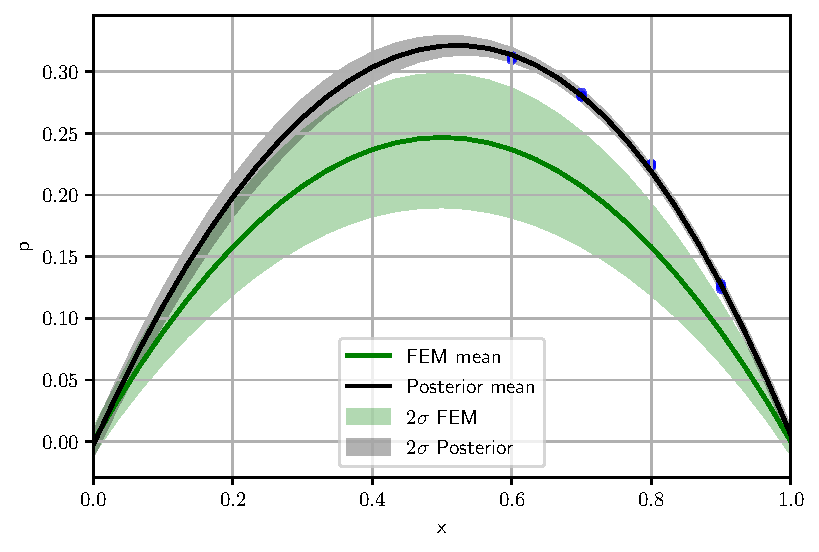
\includegraphics[width=1\linewidth]{pics/1DPost_RightSide.pdf}
	\caption{If data is measured only on one side of the domain the overall shape of the FEM prior still remains but the variance changes according to the presence of data in a region of the domain.}
		\label{fig:DOneSided}
	\end{subfigure}%
	\begin{subfigure}[t]{.5\textwidth}
	\centering
	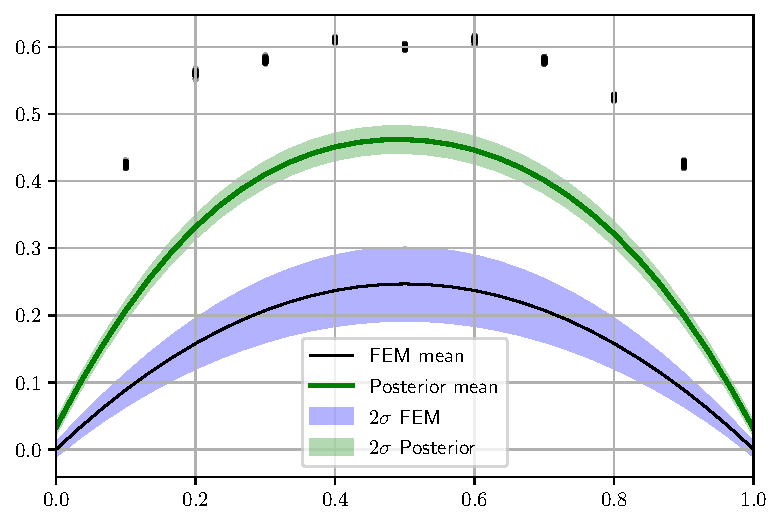
\includegraphics[width=1\linewidth]{pics/DataPriorMismatch.pdf}
\centering
\caption{Per observation point 50 individual observations were used with a standard deviation of $2.5e-3$. 30 Elements.}
\label{fig:DataPriorConflict}
	\end{subfigure}

\caption{Taking observations slightly out of the prior confidence bands works, but the further away the measurements are taken, the more weight is on thr prior and the data is not matched.}
\end{figure}
%
\section{2D Vibroacoustics Example}
Based on the knowledge of the methods gained in the simple 1D example, the methods are now applied on a 2D vibroacoustics problem. At first, the FEM prior has to be constructed. This is done by introducing the Neumann boundary on the left side of the domain as a GP. Afterwards, synthetic observation data can be generated and the prior is conditioned in order to form the posterior.

\paragraph{Generating Fake Data}
To generate a posterior, the prior needs to be conditioned on measured data. In this thesis no real measurements have been taken. Instead, fake measurement data is created. One advantage of using fake measurements at first is that the ground truth is very well known: Any number of measurements can be taken at any location in the domain, i.e. there is a whole GP available for the ground truth with which the posterior can be compared.
That ground truth can be created in different ways. Here, it is based on the FEM prior: The prior is modified using some predifined parameters which are then to be estimated by statFEM. Scaling the prior GP by a certain factor $\rho$ leads to a new GP without any model error. Superimposing the prior with a function or another GP leads to a new GP with some model error.

From the generated ground truth, observations have to be taken. Here, two methods have been applied to do so: The first one is to choose the sensor locations randomly in the domain. Another method is an "active learning" approach: The first sensor location is chosen randomly. After calculating the posterior GP, the next sensor location is placed at the point of the highest variance. This should lead to a quicker convergence to a low level of variance.


\paragraph{FEM setup}
Table \ref{tab:FEMSetup} shows the parameters used to setup the FEM mesh.  
\begin{table}[]
\centering
\caption{The parameters used to setup the FEM mesh.}
\label{tab:FEMSetup}
\begin{tabular}{@{}ccccc@{}}
\toprule
$n_a$ & $n_b$ & basis function type & basis function degree & domain               \\ \midrule
24    & 24    & Lagrange            & 1                     & square, $1\times 1$m \\ \bottomrule
\end{tabular}
\end{table}
The material parameters are defined in Table \ref{tab:MatSetup}.
\begin{table}[]
\centering
\caption{The material and frequency constants in the PDE have been set to these values. The frequency was varied in one chapter but kept constant in most parts of the thesis.}
\label{tab:MatSetup}
\begin{tabular}{@{}ccc@{}}
\toprule
$\rho_0${[}kg/m**3{]} & $c${[}m/s{]} & $f${[}Hz{]} \\ \midrule
1.2                   & 340          & 500         \\ \bottomrule
\end{tabular}
\end{table}
The numbers of elements in each direction $n_a$ and $n_b$ have been chosen to be $24\times 24$ because the used workstation was only able to compute the problem up to this amount of elements in an acceptable time. As a thumb rule, 6 nodes per wave length $\lambda$ are usually used to be able to properly resolve the solution. \cite{Marburga} With an edge length of the domain of $1m$, 24 nodes can resolve 4 wave lengths of $0.25m$ each. Therefore, for the maximum accurately resolved frequency there holds 
\begin{equation}
f = \frac{c}{\lambda} = \frac{340m/s}{0.25m} = 1360Hz \;,
\end{equation}
hence all examples in this thesis are going to be solved for frequencies less than $1360Hz$.
The final mesh can be seen in Figure \ref{fig:meshFEM}.
\begin{figure}[!ht]
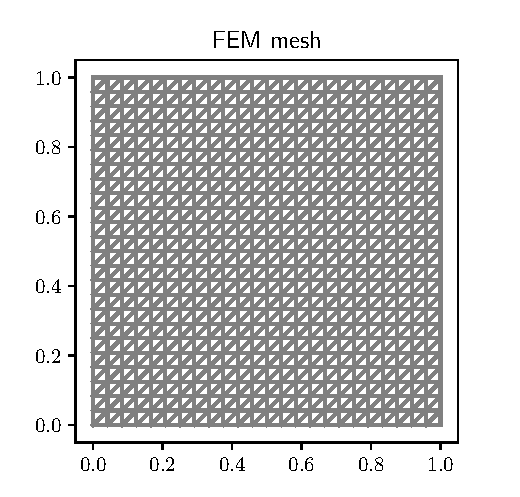
\includegraphics[width=0.5\textwidth]{pics/mesh.pdf}
\centering
\caption{The chosen mesh consists of 24 elements per dimension. Linear basis functions are chosen whcih results in three nodes per element.}
\label{fig:meshFEM}
\end{figure}


\paragraph{Experimental Design}
The following numerical experiments are conducted and the results are discussed in the next chapters.

\begin{itemize}
  \item Formation of a FEM prior GP, approximation of variance and mean function
  \item Conditioning of the FEM prior on 1 sensor location with 1 observation taken from an FEM prior sample. Expected outcome: Variance drop in the region around the sensor, mean function remains unchanged, model inadequacy GP insignificant
  \item Increase of the number of sensor locations and observations: A further variance drop is expected.
  \item Same as before but measurements taken on a 75 \% scaling of the FEM prior sample. Expected outcome: Scaling factor of $\rho = 0.75$ should be found, model inadequacy GP stays insignificant
  \item Alteration of the FEM prior sample in a way that a significant model inadequacy is expected. Expected outcome: Increased values for $\sigma_d$ and $l_d$ will be observed.
  \item Taking observations far beyond the FEM prior variance. An increased variance and a wrong scaling are expected.
  \item Observation only on a fraction of the domain. The overall shape should still follow the FEM prior. Variance drop in the region with measurements is expected but not in the other parts of the domain.
  \item A constant Neumann source term is chosen: The problem should reduce to an 1D equivalent.

\end{itemize}






\subsection{FEM prior}
Figure \ref{fig:FEMGP} shows how the FEM prior is formed. On the left face of the domain, the source term GP is applied. The mean and confidence bands are visible in red. Exciting the domain with the source leads to an uncertain FEM solution in the 2D domain. At $y_c = 0.7$, an arbitrary value, the domain is cut and the mean and error bands for that position are displayed in green. Clearly, uncertainty in the source leads to uncertainty in the FEM prior. A MC simulation for the variance converges to the calculated variance.
Figure \ref{fig:NeumannBC} shows the GP which is used to model the $\bar{U}$ variable in the Neumann source BC. The mean follows
\begin{equation}
\bar{U}(y) = 0.00001 \sin(\pi y) + 0.000005 \sin(2\pi y)
\end{equation}
and the Matern kernel is evaluated with $l = \mathrm{ln}(0.8)$ and $\sigma = \mathrm{ln}(9)$ to form $C_U$, so there holds
\begin{equation}
U \sim \mathcal{GP}(\bar{U},C_U) \;.
\end{equation}

\begin{figure}[!ht]
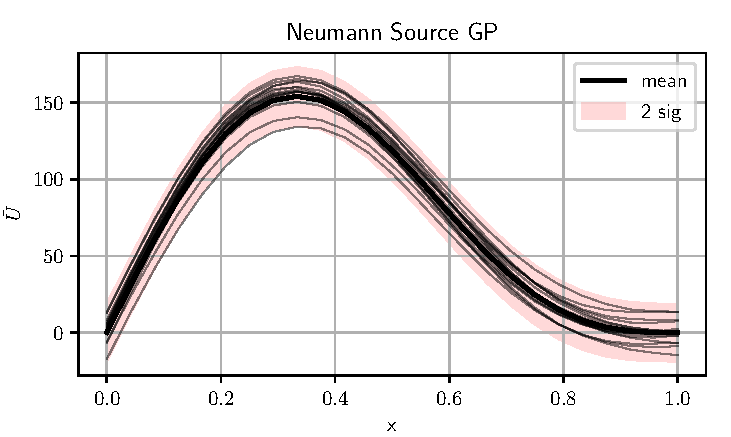
\includegraphics[width=0.8\textwidth]{pics/NeumannBC.pdf}
\centering
\caption{The Neumann BC is modeled as a GP with a harmonic mean and a Matern kernel. The mean, the $2 \sigma$ confidence band and some drawn samples are shown.}
\label{fig:NeumannBC}
\end{figure}
%
\begin{figure}[!ht]
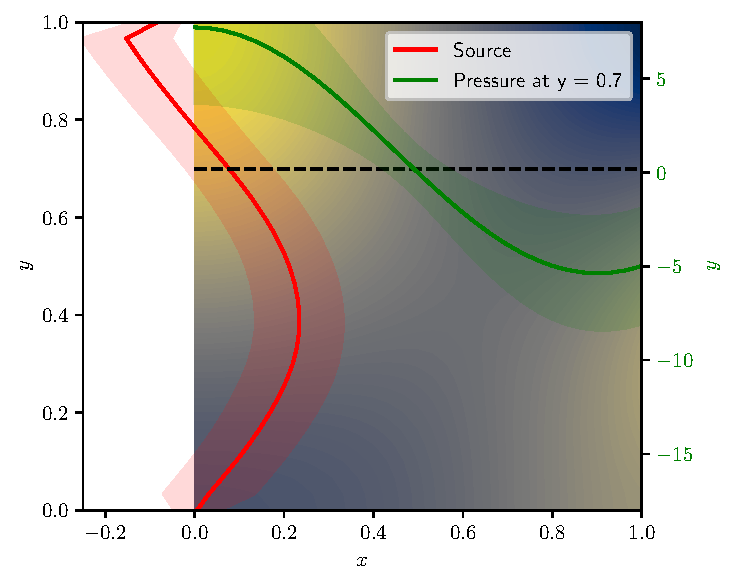
\includegraphics[width=0.8\textwidth]{pics/SolutionCustom2D.pdf}
\centering
\caption{The source GP, the mean prior and, at the cut $y=y_c$, the prior FEM GP for 222Hz. The variance around the source leads to a variance in the pressure field which is the lowest where the mean absolute pressure is the lowest.}
\label{fig:FEMGP}
\end{figure}
%
Figure \ref{fig:varFieldPrior} shows the FEM prior variance for every point in the 2D solution space for $222Hz$. It is visible that the variance in some regions is higher than in others. The regions of low variance correlate with the troughs of the mode shape.
%
\begin{figure}[!ht]
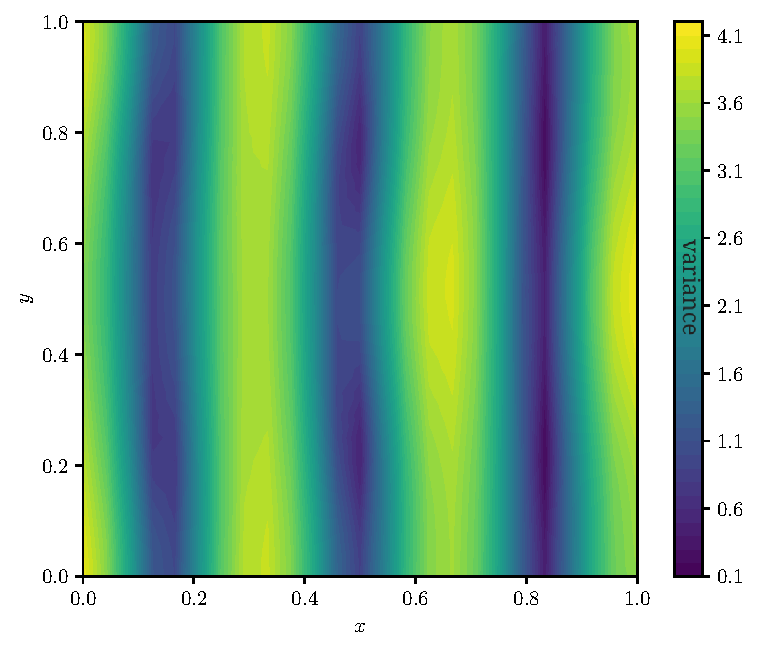
\includegraphics[width=0.6\textwidth]{pics/VarField.pdf}
\centering
\caption{The variance of the FEM prior for $500Hz$ at all points in the 2D space. Regions with high and low variance are clearly visible: Regions with high absolute pressure peaks also have a high variance. This implies that the positions of the nodal points in the mode shape are approximated very accurately.}
\label{fig:varFieldPrior}
\end{figure}
%
%Figure \ref{fig:FEMGP320} shows again an overview for the FEM prior, but for $320 Hz$. 
%
%\begin{figure}[!ht]
%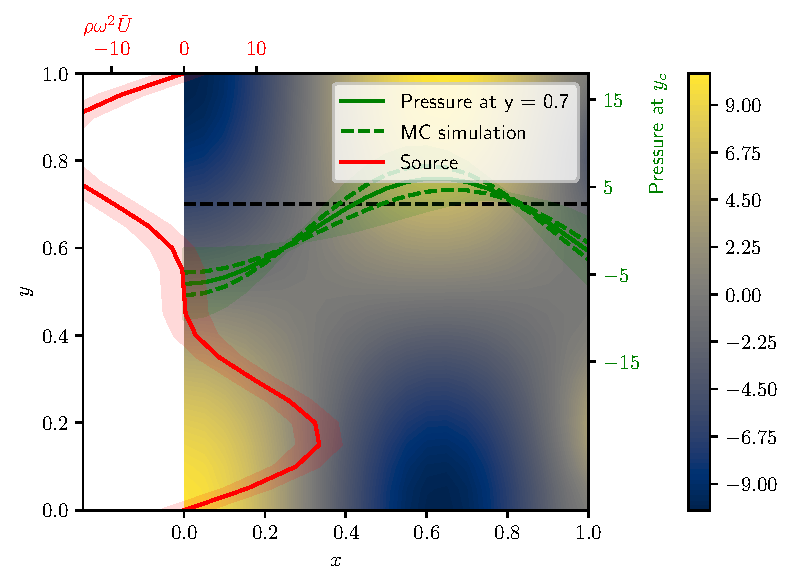
\includegraphics[width=0.7\textwidth]{../../Python/SolutionCustom320Hz.pdf}
%\centering
%\caption{The source GP, the mean prior and, at the cut $y=y_c$, the prior FEM GP for 320Hz.}
%\label{fig:FEMGP320}
%\end{figure}
%
%In Figure \ref{fig:varFieldPrior320} it is visible that the variance pattern changed to a %periodic one.
%\begin{figure}[!ht][!ht]
%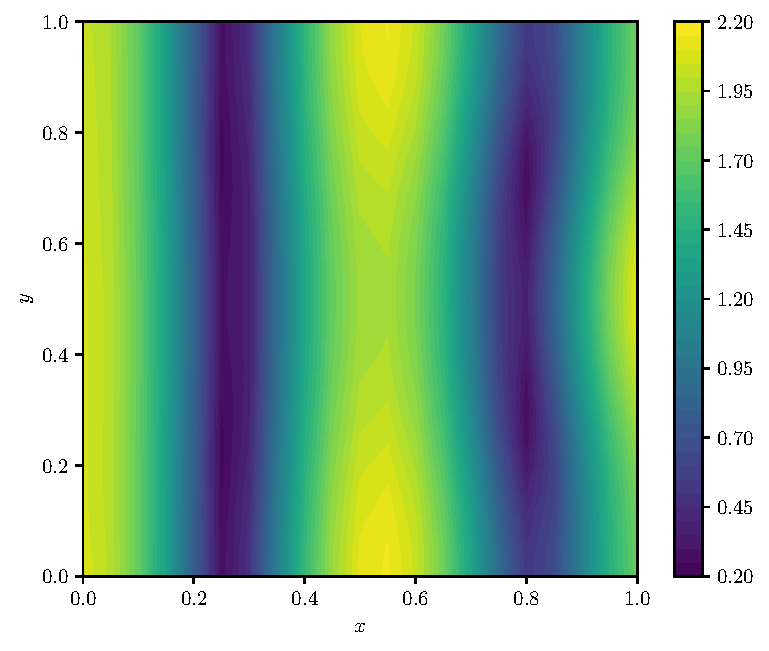
\includegraphics[width=0.6\textwidth]{../../Python/VarField320Hz.pdf}
%\centering
%\caption{The variance of the FEM prior for $320Hz$ at all points in the 2D space. Regions %with high and low variance are clearly visible.}
%label{fig:varFieldPrior320}
%\end{figure}
%


\subsection{Posterior, observations on prior sample}
For the posterior, data has to be generated or measured on which the FEM prior can be conditioned. For that, a ground truth has to be created: In the simplest case it is a sample from the FEM prior. The next step is scaling the sample. Then, to make the problem more complex, the prior sample is changed in a way that it does not resemble the prior GP anymore: Model error is introduced.
\paragraph{Hypothesis}
As stated and described in \cite{rasmussen2006}, the variance is supposed to become lower with increasing the number of sensor locations and/or observations. It is expected that this behavior also holds for the Helmholtz problem. Also, it is expected that the mean of the posterior GP gets closer to the observations the more data is introduced. For both observations with and without artificially introduced model error, statFEM is expected to form a suitable posterior which modifies the FEM prior to account for the data. The generated hyperparameters for the posterior GP are expected to reflect the scaling and/or model error.


\paragraph{Without Model Error}
As a first example, a sample of the FEM prior is used as a ground truth from which observations are made. It is basically the "true solution" which is measured. A random measurement error of $e \sim \mathcal{U}(\num{-2.5e-3}, \num{2.5e-3})$ is added to the artificial measurement values. At first only one sensor location is chosen and one measurement is taken. Then it is shown that introducing more sensor locations and measurements lead to an overall smaller variance. The sensor locations are chosen randomly. It is expected that the scaling hyperparameter $\rho$ is approximated as close to $1$ whereas $\sigma_d$ becomes very small because measuring from the FEM prior means measuring from a possible solution of the prior and therefore no model error. Figure \ref{fig:100proc_no_d} shows that this holds approximately. %A $\sigma_d$  of $0.1010101010?!$ was determined.

In Figure \ref{fig:100proc_no_d} the variance field in the calculation domain is shown for different combinations of the number of sensor locations $n_p$ and the number of observations $n_o$. It is visible that the variance gets lower the more sensor locations are introduced and the more observations are made. For easier comparison, the $l_2$ norm for the whole domain is given in each plot.
\begin{figure}[!ht]
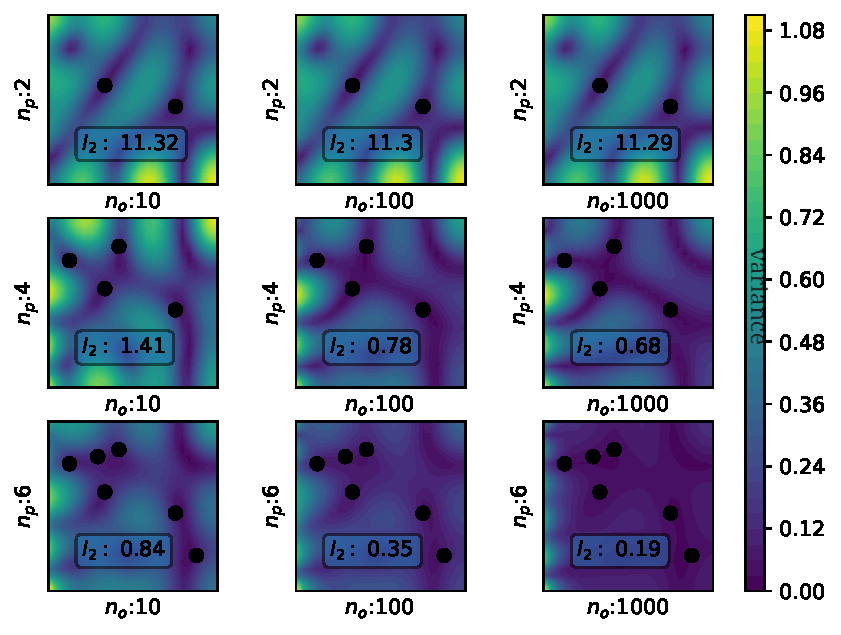
\includegraphics[width=.9\textwidth]{../../Python/Results/2D/100procent_no_d/VarField_Posterior.pdf}
\centering
\caption{The variance of the posterior for $500Hz$ at all points in the 2D space for different combinations of sensor and observation numbers. Regions with high and low variance are clearly visible. Where sensor locations are introduced, the variance gets smaller in patterns around the location all over the domain. Adding more sensor locations induces a thinner mesh of patterns. The more observations are taken per sensor, the smaller the overall variance becomes, which reflects in the specified l2 norm for it.}
\label{fig:100proc_no_d}
\end{figure}
Also, it is discernible that where a sensor location is introduced, the variance does not only get lower in the immediate surrounding of the sensor but rather in patterns which have their origin at the sensor location. The more sensors are introduced the more complicated the pattern becomes until no pattern is visible anymore. Even with large $n_p$ and $n_o$, there is still the variance of the Neumann boundary visible in the left side of the domain.
Table \ref{tab:rho100p_nod} shows the approximated values for $\rho$ for each case. It is always close to $1$. The small difference is probably due to the introduced measurement noise. The values for $\sigma_d$ are always very small which corresponds with the fact that no model error was introduced.

\begin{table}[]
\centering
\caption{For a $100\%$ scaling and no introduced model error, $\rho$ is close to $1$ for every case, which is expected for a direct FEM prior sample as ground truth. The model error parameters are close to zero which is expected, because no model error was introduced.}
\label{tab:rho100p_nod}
\begin{tabular}{@{}cccc@{}}
\toprule
  & $n_o = 10$ & $n_o = 100$ & $n_o = 1000$ \\ \midrule
$n_p = 2$           & $\rho=1.013$, $\sigma_d=0.016$      & $\rho=1.022$, $\sigma_d=0.011$      & $\rho=1.001$, $\sigma_d=0.034$         \\
$n_p = 4$           & $\rho=0.989$, $\sigma_d=0.019$      & $\rho=0.977$, $\sigma_d=0.022$      & $\rho=0.974$, $\sigma_d=0.007$        \\
$n_p = 6$           & $\rho=0.963$, $\sigma_d=0.008$     & $\rho=0.974$, $\sigma_d=0.008$      & $\rho=0.960$, $\sigma_d=0.008$        \\ \bottomrule
\end{tabular}
\end{table}
%

\subsection{Posterior, observations on scaled prior sample}
For a $75\%$ scaling of an FEM prior realization as ground truth the scaling parameter $\rho$ is correctly approximated to be close to $0.75$ in every case, see Table \ref{tab:rho75p_nod}. Again, the model error is very low due to the low $\sigma_d$, which is expected.
\begin{table}[]
\centering
\caption{For a $75\%$ scaling and no introduced model error, $\rho$ is close to $0.75$ for every case, which is expected for a $75 \%$ scales FEM prior sample as ground truth. The model error is close to zero.}
\label{tab:rho75p_nod}
\begin{tabular}{@{}cccc@{}}
\toprule
  & $n_o = 10$ & $n_o = 100$ & $n_o = 1000$ \\ \midrule
$n_p = 2$           & $\rho=0.741$, $\sigma_d=0.011$      & $\rho=0.746$, $\sigma_d=0.010$      & $\rho=0.735$, $\sigma_d=0.007$         \\
$n_p = 4$           & $\rho=0.750$, $\sigma_d=0.011$      & $\rho=0.753$, $\sigma_d=0.010$      & $\rho=0.739$, $\sigma_d=0.025$        \\
$n_p = 6$           & $\rho=0.764$, $\sigma_d=0.012$     & $\rho=0.762$, $\sigma_d=0.010$      & $\rho=0.764$, $\sigma_d=0.007$        \\ \bottomrule
\end{tabular}
\end{table}
%
Scaling the FEM prior sample by $75\%$ should lead to a scaling factor of $\rho = 0.75$. Figure \ref{fig:75proc_no_d_overview} shows that this is approximately the case.

\begin{figure}[!ht]
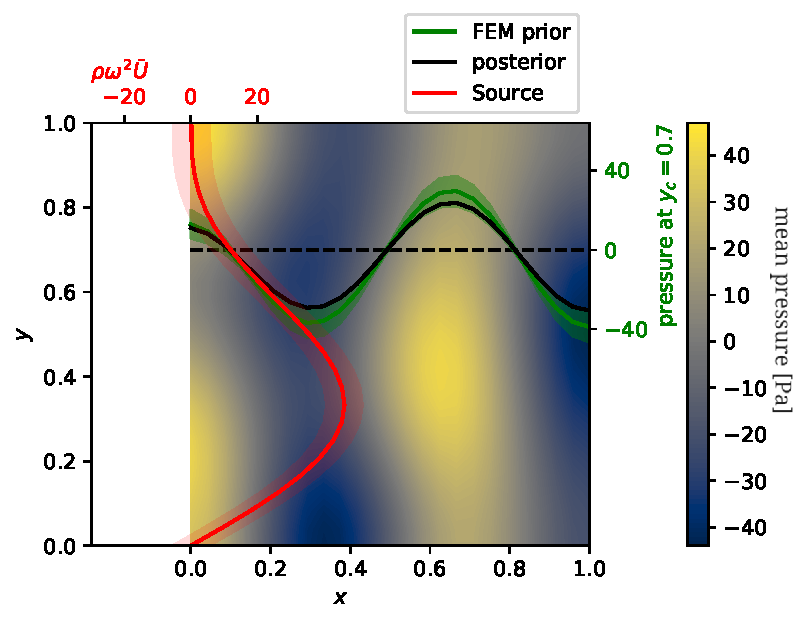
\includegraphics[width=0.8\textwidth]{../../Python/Results/2D/75procent_no_d/SolutionCustomPosterior.pdf}
\centering
\caption{The variance of the posterior for $500Hz$ at all points in the 2D space for different combinations of sensor and observation numbers. Sampled from a $75\%$ scaling. Regions with high and low variance are clearly visible.}
\end{figure}
\label{fig:75proc_no_d_overview}

The 2D field shows the mean posterior whereas the green curve describes a cut through the FEM prior field which gives insight on the variance of the prior. In black, a cut through the posterior mean is shown. The $75\%$ scaling is visible.
%
Figure \ref{fig:75proc_no_d} shows the variance fields for the posterior when taking measurements from the $75\%$ scaling. Still, the variance gets lower with higher $n_p$ and $n_o$.

\begin{figure}[!ht]
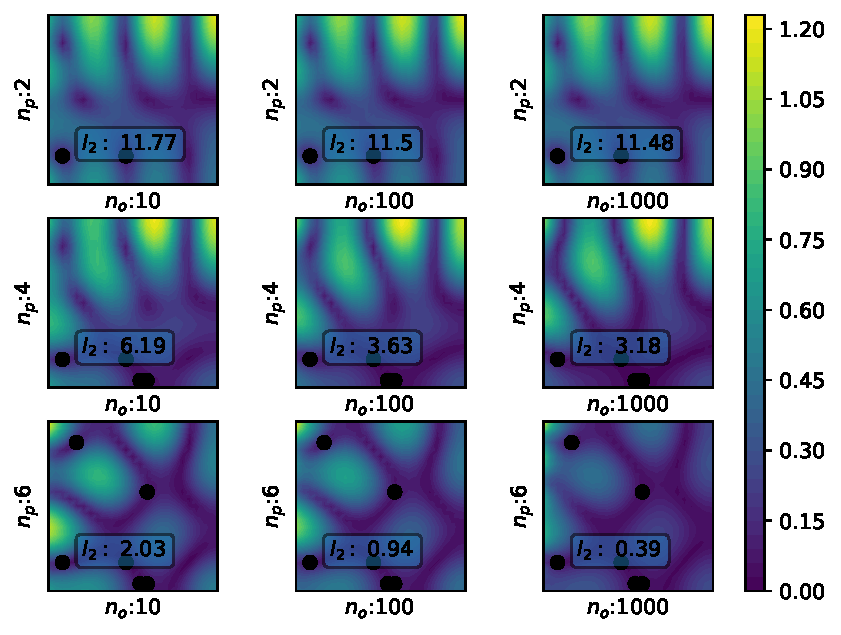
\includegraphics[width=.9\textwidth]{../../Python/Results/2D/75procent_no_d/VarField_Posterior.pdf}
\centering
\caption{The variance of the posterior for $500Hz$ at all points in the 2D space for different combinations of sensor and observation numbers. Sampled from a $75\%$ scaling. Regions with high and low variance are clearly visible. Although the observations were taken from the scaled sample, the variance quickly gets smaller with more sensors and observations.}
\label{fig:75proc_no_d}
\end{figure}
%
Figure \ref{fig:75proc_no_d3d} shows ten sampled points in space and the FEM prior on the left as well as the corresponding posterior on the right. It is visible that the posterior matches the data exactly.
%
\begin{figure}[!ht]
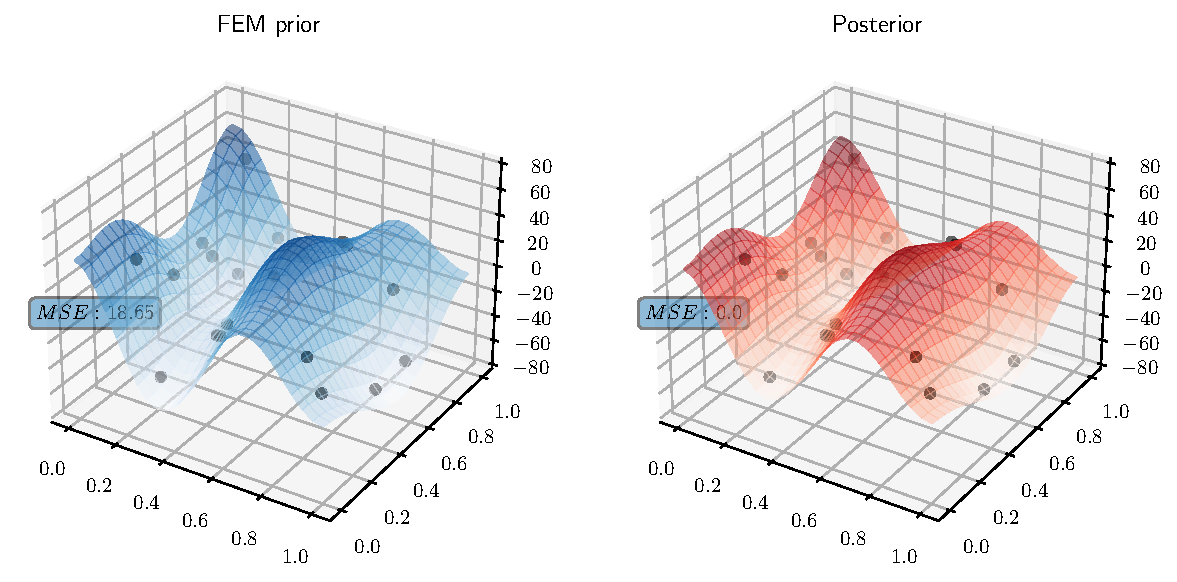
\includegraphics[width=1\textwidth]{../../Python/Results/2D/75procent_no_d/3dMSE.pdf}
\centering
\caption{See the \href{https://github.com/herluc/Masterarbeit/blob/master/MA_LucasHermann/Python/Results/2D/75procent_no_d/3DMSE.gif}{Animation} to see the differences better. With observations on a 75\% scaling of the FEM prior and no other introduced model error, the posterior is able to match the data with an MSE of $0.0$. }
\label{fig:75proc_no_d3d}
\end{figure}


\subsection{Posterior, observations on altered prior sample}
In a second example, the ground truth to measure from was again the FEM prior but with certain changes. In a certain region of the domain the values of the FEM prior sample were changed according to a 2D Gaussian, resulting in a clearly visible deviation. That deviation should lead to a larger model inadequacy term whereas the scaling factor should stay roughly the same. Figure \ref{fig:ObsPat} shows, how observations with model error are created. At first, a rescaling pattern is created. It comprises values of around one and is then multiplied with a sample from the FEM prior. This new, altered, sample is now used to make observations on. These observations differ from the standard prior sample by the amount specified in the rescaling pattern. Note that if the prior would only have been rescaled by a constant factor throughout the domain, no model error would have been introduced: statFEM would yield a fitting scaling parameter $\rho$ and model inadequacy hyperparameters of close to zero. Here, it is forced to work with all three hyperparameters since a simple constant rescaling would not be enough. The non-constant rescaling follows
\begin{equation}
K_{res} \odot K_{samp} = K_{obs}
\end{equation}
where $K_{res}$ is the matrix which contains the values of the rescaling pattern and $K_{samp}$ is a sample drawn from the FEM prior GP. An element-wise multiplication yields $K_{obs}$, the resulting matrix to draw samples from.
\begin{figure}[!ht]
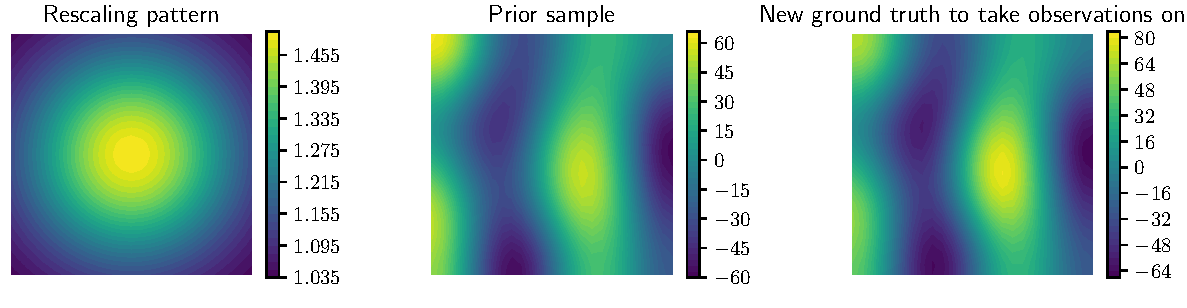
\includegraphics[width=1\textwidth]{pics/ObsPattern.pdf}
\centering
\caption{Multiplying a prior sample with a rescaling pattern leads to a new ground truth with model error. The pattern strongly scales the sample in the middle of the domain and less strongly on the corners.}
\label{fig:ObsPat}
\end{figure}

The pattern is described by
\begin{equation}
z = 1+\frac{0.5}{\mathrm{exp}(5((x-0.5)^2 + (y-0.5)^2))} \;.
\end{equation}

As visible in Figure \ref{fig:ObservationPriorPost}, the observations follow the general shape of the prior but deviate slightly in terms of magnitude. It is now expected that statFEM is able to form a posterior which resembles the observed data more closely while maintaining the general shape of the FEM prior.
\begin{figure}[!ht]
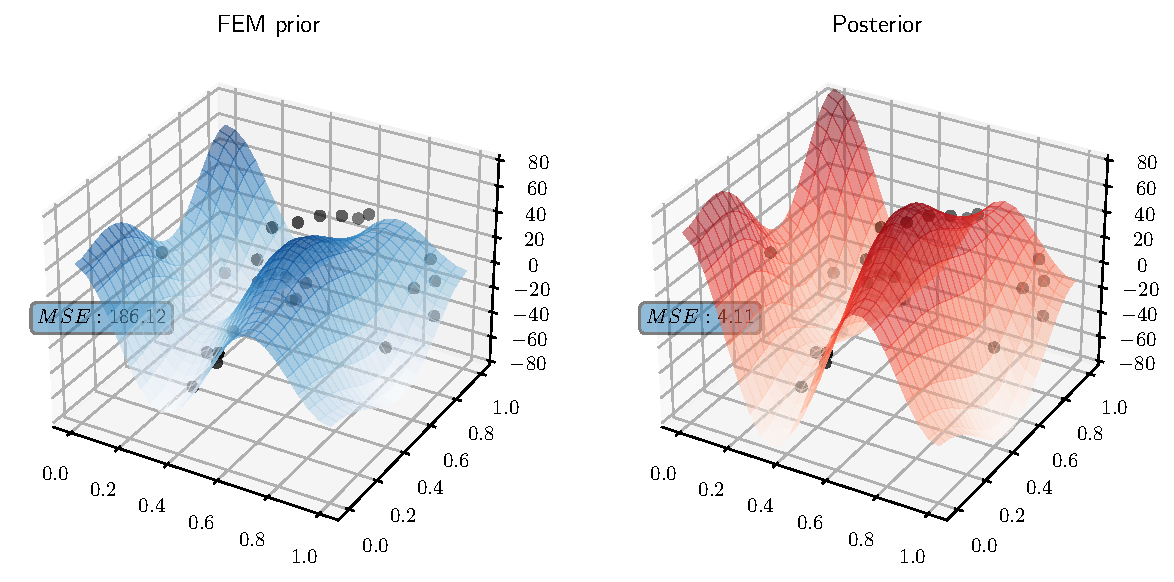
\includegraphics[width=1\textwidth]{pics/3dTest.pdf}
\centering
\caption{On the left: A sample from the FEM prior and the observations. It is visible that the points, first if al those in the middle, are not coincident with the surface formed by the prior. The mean squared error (MSE) is given and rather high. On the right: The posterior now fits to the observation data which is also reflected in a lower MSE.}
\label{fig:ObservationPriorPost}
\end{figure}
As it is hard to see by eye in the plots, the difference of the magnitude of the observations compared to the prior and the posterior are cumulated in the mean squared error (MSE). As expected, the MSE for the FEM prior is comparatively high. statFEM manages to find the best hyperparameters to find a posterior which matches the data as close as possible. 
This is also reflected in the generated hyperparameters: Since the rescaling pattern only comprises values greater than one, the overall prior is rescaled with $\rho > 1$. But, to account for the non-constant rescaling, also the model inadequacy hyperparameters $\sigma_d$ and $\l_d$ are now much larger than in the example without model error, as it is visible in Table \ref{tab:100procWithError}.
\begin{table}[!ht]
\centering
\caption{Hyperparameters for the case of observed data with a model error. The solution is scaled by around 20\% and the hyperparameters describing the model inadequacy are not close to zero anymore.}
\label{tab:100procWithError}
\begin{tabular}{@{}lccc@{}}
\toprule
                            & $n_o = 10$                      & $n_o = 100$                     & $n_o = 500$                     \\ \midrule
\multirow{2}{*}{$n_p = 15$} & $\rho=1.206$, $\sigma_d=3.230$, & $\rho=1.206$, $\sigma_d=2.213$, & $\rho=1.181$, $\sigma_d=3.648$, \\
                            & \multicolumn{1}{l}{$l_d=0.471$} & \multicolumn{1}{l}{$l_d=0.471$} & \multicolumn{1}{l}{$l_d=0.556$} \\
\multirow{2}{*}{$n_p = 30$} & $\rho=1.125$, $\sigma_d=3.333$  & $\rho=1.220$, $\sigma_d=3.019$  & $\rho=1.239$, $\sigma_d=2.848$  \\
                            & \multicolumn{1}{l}{$l_d=0.147$} & \multicolumn{1}{l}{$l_d=0.154$} & \multicolumn{1}{l}{$l_d=0.105$} \\
\multirow{2}{*}{$n_p = 45$} & $\rho=1.284$, $\sigma_d=7.071$  & $\rho=1.195$, $\sigma_d=7.633$  & $\rho=1.181$, $\sigma_d=4.157$  \\
                            & \multicolumn{1}{l}{$l_d=0.343$} & \multicolumn{1}{l}{$l_d=0.429$} & \multicolumn{1}{l}{$l_d=0.301$} \\ \bottomrule
\end{tabular}
\end{table}
%
It is visible in Figure \ref{fig:100procent_d} that the variance doesn't become smaller for 10 observations when the number if sensor locations is changed from 4 to 6. Because of the small number of sensors and observations, the model error couldn't be resolved adequately which lead in turn to the higher variance. This has already been shown for the 1D example in Figure \ref{fig:ModErrNoModErr1D} and is therefore expected. The effect can also be explained in another way: As already discussed, Bayesian regression always favors a less complex model over a more complex one. If now only very few sensors are used, it would be possible to find a posterior which adequately describes the data by only scaling the prior using the scaling hyperparameter $\rho$. The other hyperparameters could stay unchanged, i.e. zero, resulting in a simple model. If then more sensors are introduced, it is not possible to describe the data by only scaling the prior, so the model inadequacy part $d$ comes into play. The posterior variance quickly converges in this case by observing more data per sensor.
\begin{figure}[!ht]
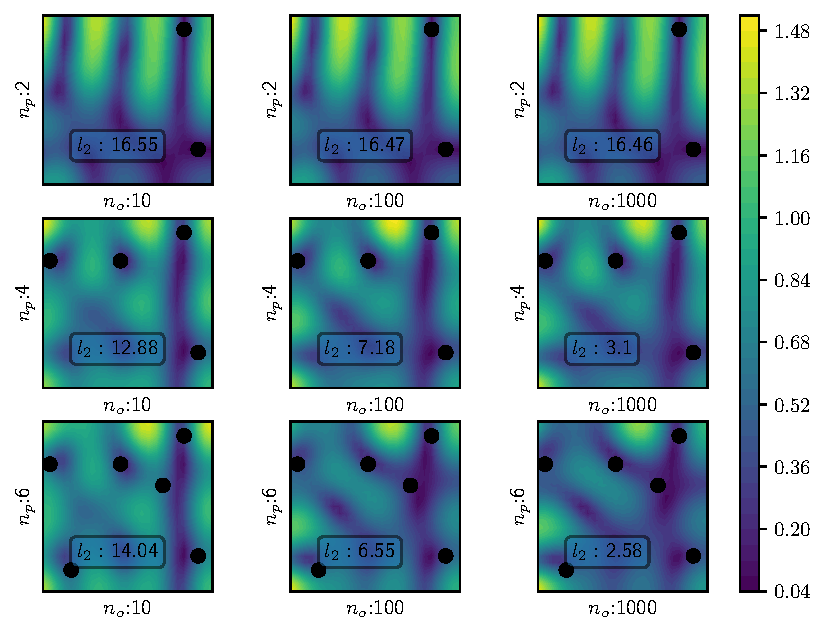
\includegraphics[width=.9\textwidth]{../../Python/Results/2D/100procent_d/VarField_Posterior.pdf}
\centering
\caption{Introducing model error leads to a higher variance for a small number of sensor locations.}
\label{fig:100procent_d}
\end{figure}
Figure \ref{fig:100procent_d_more} shows that this is the case: Introducing more sensor locations leads to the typical behavior of decreasing variance with more sensors and observations.
\begin{figure}[!ht]
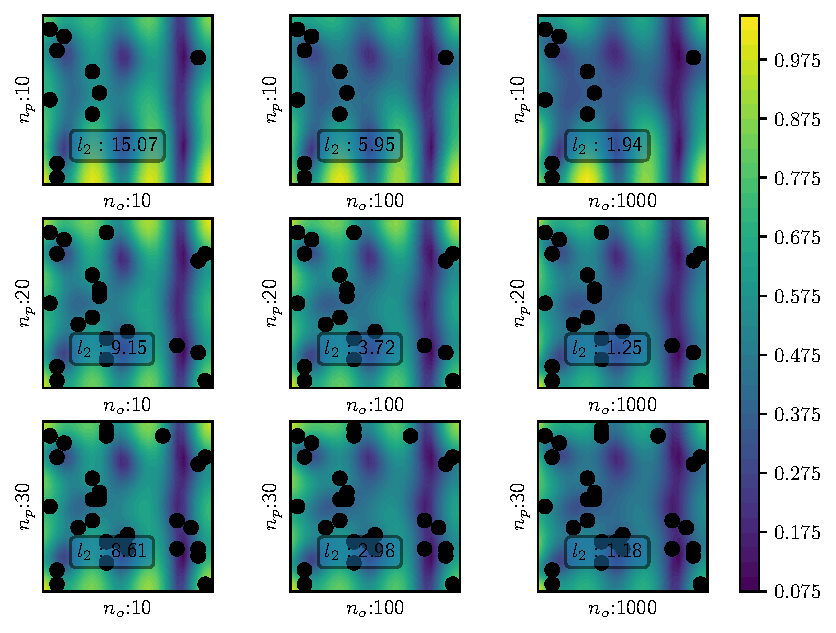
\includegraphics[width=.9\textwidth]{../../Python/Results/2D/100procent_d/VarField_PosteriorMoreSensors.pdf}
\centering
\caption{Introducing more sensor locations, it is now visible that the variance goes down with mmore observations and more sensors, just as expected.}
\label{fig:100procent_d_more}
\end{figure}


\subsection{Prior-Data Conflict}
As already shown for the 1D example, as soon as data is observed far outside the confidence region of the prior, i.e. there is a prior-data conflict, the inference doesn't yield accurate results anymore. Figure \ref{fig:3dPriorDataConf} shows that especially the observations in the middle of the domain are not matched and that the MSE remains very high.
%
\begin{figure}[!ht]
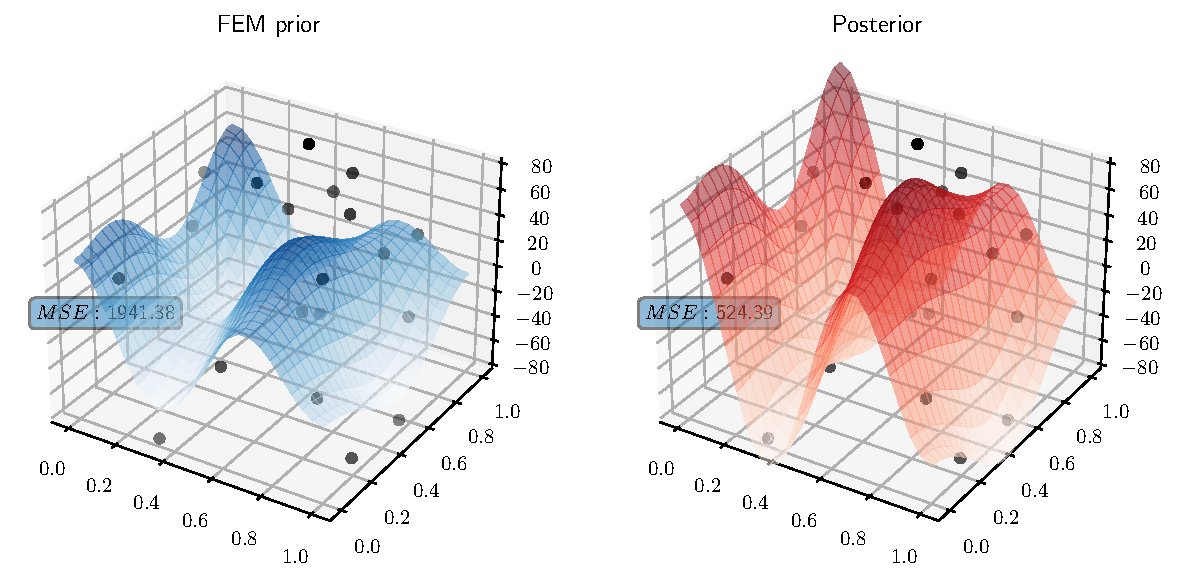
\includegraphics[width=1\textwidth]{../../Python/Results/2D/prior_data_conflict/3dMSE.pdf}
\centering
\caption{See the \href{https://github.com/herluc/Masterarbeit/blob/master/MA_LucasHermann/Python/Results/2D/prior_data_conflict/3DMSE_conflict.gif}{Animation} to see the differences better. If data is observed far outside the confidence intervals of the prior, the prosedure is not able to match the posterior perfectly to the data. More sensor locations and more observations are necessary to improve the result.}
\label{fig:3dPriorDataConf}
\end{figure}
%
Figure \ref{fig:PriorDataConfPOST} shows the FEM prior compared to the posterior. Obviously, a high scaling factor was found, but also the variance didn't get as low as for other examples in which there was no prior-data conflict. This is in agreement with the results of the 1D example and therefore expected.
%
\begin{figure}[!ht]
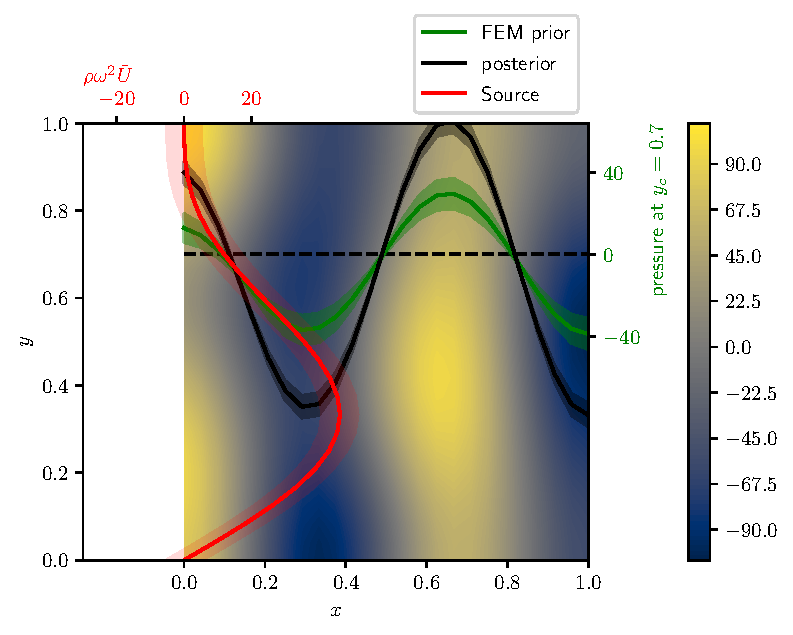
\includegraphics[width=.8\textwidth]{../../Python/Results/2D/prior_data_conflict/SolutionCustomPosterior.pdf}
\centering
\caption{}
\label{fig:PriorDataConfPOST}
\end{figure}
The approximated hyperparameters can be found in Table \ref{tab:PriorDataConf}.
%
\begin{table}[!ht]
\centering
\caption{For the prior-data conflict, a comparatively high scaling factor $\rho$ is found. The standard deviation hyperparameter for the model inadequacy term $d$ is also higher than in other examples.}
\label{tab:PriorDataConf}
\begin{tabular}{@{}llcc@{}}
\toprule
                                                                & $\rho$ & $\sigma_d$ & $l_d$ \\ \midrule
\begin{tabular}[c]{@{}l@{}}$n_p = 20$,\\ $n_o = 1$\end{tabular} & 1.405  & 17.505     & 0.167 \\ \bottomrule
\end{tabular}
\end{table}



\subsection{Variations in the Neumann BC}
If instead of a sinusoidal source a flat one is chosen, the solution changes significantly, see Figure \ref{fig:FEMGPFlat320}. Certain mode shapes can be excited more strongly by using a corresponding boundary function.
\begin{figure}[!ht]
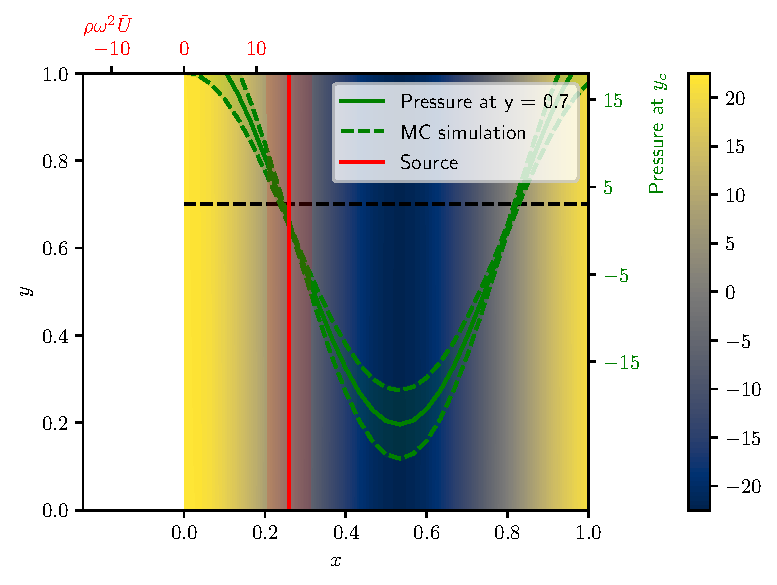
\includegraphics[width=0.8\textwidth]{../../Python/SolutionCustomFlatSource320.pdf}
\centering
\caption{The source GP, the mean prior and, at the cut $y=y_c$, the prior FEM GP for 320Hz.}
\label{fig:FEMGPFlat320}
\end{figure}
%
The variance field, on the other hand, does not change significantly, see Figure \ref{fig:varFieldPriorFlat320}.
\begin{figure}[!ht]
\includegraphics[width=0.7\textwidth]{../../Python/VarFieldFlatSource320.pdf}
\centering
\caption{The variance of the FEM prior for $320Hz$ at all points in the 2D space. Regions with high and low variance are clearly visible.}
\label{fig:varFieldPriorFlat320}
\end{figure}
With the FEM prior, data can now be introduced to form the posterior.


\chapter{Discussion and Conclusion}
After a review of the used method and its theoretical foundation, i.e. first of all Gaussian Process regression, a statFEM approach for vibroacoustics was developed and numerical experiments were carried out to prove that the software which was programmed for this thesis works. 

At first, the simple text-book example of solving the Poisson equation in a 1D domain was treated. The same parameters as in \cite{girolami2021} were chosen and its results could be replicated: The source term was modeled as a GP and through a first Bayesian inference step the FEM prior GP could be formed. A second Bayesian inference step then lead to the posterior GP: The prior was conditioned on artificial measurement data. as in the reference, observing more data on more sensor locations lead to a more accurate representation of the data as well as to a smaller variance. Additionally, the limits of the method were examined by choosing measurement data which has either been observed only on a part of the domain or far outside the prior confidence bands. For the former, the method was able to form a plausible posterior with small variance in the region with data and larger variance in the other parts of the domain. The latter demonstrated a prior-data conflict: An accurate representation of the data would by very costly from a numerical point of view.

The same experiments have been conducted for a more complex, 2D Helmholtz equation example. The numerical setup is a first approximation of an interior structural acoustic coupling problem. In such a problem, there is some kind of two-dimensional structure, like a plate, which emits sound into a three-dimensional cavity. Without loss of generality, that problem was reduced to a 2D problem in this thesis which basically resembles a cross sectional view of the cavity and the plate. Hence, there is a 1D sound emitter on the boundary of a 2D domain in which the sound is radiated and reflected. The 1D emitter was completely modeled as a GP with a Matern kernel function:  Beam- and/or plate-theory wasn't used here.  As in the 1D example, an FEM prior was formed using the source GP which was, contrary to the 1D example, defined in a boundary condition. It was possible to condition the prior on artificial measurement data: The correct scaling factors were approximated and artificial model error could be resolved. Again, a prior-data conflict could be provoked, which was expected. 

Due to the promising results, statFEM appears to be a useful method to incorporate sound pressure measurements into a given FEM analysis of a vibroacoustic problem. However, further research should be conducted: A more realistic source GP has to be found. Dirichlet kernel functions appear promising because they are derived using a fourier expansion which makes them inherently based on harmonic functions, by which the mode shapes of vibrating plates are usually modeled. Also, it could be possible to model a complete fluid/structure coupling problem in which the material or geometrical parameters of, for instance, a radiating plate can be modeled as a GP. Another very important step towards a more realistic model is to introduce impedance boundary conditions. Those, or respectively their parameters, should also be modeled as GPs. 

statFEM for vibroacoustics could be useful for current research: Lately, universities conduct research on new kinds of airplanes. This involves big and complex FEM models which are often reduced to the bare minimum of information. That model-to-reality mismatch could be reduced by taking a rather small amount of measurements in a real environment to condition the FEM model on. 



\printbibliography


%\begin{thebibliography}{4}
%
%\bibitem{campolina}
%5Campolina, B.: Vibroacoustic modelling of aircraft double-walls with structural links using %tatistical
%Energy Analysis (SEA). Acoustics [physics.class-ph]. Université de Sherbrooke; Université %Pierre
%et Marie Curie - Paris VI (2012)

%\bibitem{Langer2019}
%Langer, S.C., Blech, C.: Cabin noise prediction using wave‐resolving aircraft models. Proc. %Appl. Math. Mech., Vol. 12 (1) (2019): e201900388. doi:10.1002/pamm.201900388

%\bibitem {Yaghoubi:2017} Yaghoubi, V., Marelli, S., Sudret, B., Abrahamsson, T.: Sparse %polynomial chaos expansions of frequency response functions using stochastic frequency %transformation, Probabilistic Engineering Mechanics, volume 48, pages 39-58 (2017)
%\end{thebibliography}

\end{document}
